
\documentclass[draft]{scrbook}

\usepackage[
  bibresource=references.bib,
  bibstyle=alphabetic,
]{preamble-thesis}

%\includeonly{content/introduction}
%\includeonly{content/preliminaries}
\includeonly{content/contextdls}
%\includeonly{content/mapping}
%\includeonly{content/jconht}
%\includeonly{content/conclusions}

\title{Formal Semantics for Models with Meta-Predicates}
\author{Stephan Böhme}
\degree{Doktoringenieur (Dr.-Ing.)}

\defensedate{DD.\ Monat 2017}

\supervisor{Prof.\ Dr.-Ing.\ Franz Baader}
\secondsupervisor{Prof.\ Dr.\ rer.\ nat.\ habil.\ ??? ?????}
\secondsupervisoruniversity{University of ???}

\handedin{im April 2017}

\begin{document}

General ToDos:\bigskip

\todo[inline]{check for iff}
\todo[inline]{check for \textasciitilde{} before \textbackslash{}cite}
\todo[inline]{check for \textasciitilde{} before \Bmc and so on}
\todo[inline]{check for \textasciitilde{} before \textbackslash{}ref}
\todo[inline]{check for ``i.e.'' with correct spacing, see \url{https://en.wikibooks.org/wiki/LaTeX/Tips_and_Tricks}}
\todo[inline]{all referenced chapters, sections, subsections, definitions, lemmas, theorems,
  examples capitalized?}
\todo[inline]{Großschreibung bei Titel von Definition (erste Buchstabe immer groß, rest klein)}
\todo[inline]{Spacing after macros, i.e.\ dl names and \OCR, etc.}
\todo[inline]{Bib in ToC}
\todo[inline]{paragraph in chapter 2 about NI, UNA, nominals and  $\top\sqsubseteq\{a\}$ is inconsistent.}
\todo[inline]{search source code for \textbackslash{}hl macro}
\todo[inline]{use \Hmc if it is an \Msig-interpretaion}
\todo[inline]{say somewhere what restricted type means}
\todo[inline]{What's about \SHOIQ in section \ref{sec:case-el}?}
\todo[inline]{In section \ref{sec:case-el}, are the \EL-LTL papers correctly cited?}
\todo[inline]{References: Months?}
\todo[inline]{define fresh names in preliminaries}
\todo[inline]{range or image -- be consistent!}
\todo[inline]{nat numbers with 0 or without 0, sollte das irgendwo stehen?}

\frontmatter
\pagestyle{empty}

\begin{titlepage}
    \begin{center}
        \setstretch{2}
        \textbf{\textsf{\huge \thetitle}}%\todo{
          %\textbf{Context Reasoning for Role-Based Models}
          %Context Reasoning for Models with Meta-Predicates? 
          %Automated Reasoning in Context-Aware ... ?
          %Two-Dimensional Description Logics for Reasoning in Role-based Models
          %Two-Dimensional Description Logics for Reasoning in Context-Dependent Domain Models
        %}
        \\
        \setstretch{1}
        \bigskip\bigskip\bigskip

        \selectlanguage{ngerman}

        \Large
        \textbf{Dissertation}\\
        \bigskip\bigskip

        zur Erlangung des akademischen Grades\\
        \thedegree\\
        \bigskip\bigskip

        vorgelegt an der\\
        Technischen Universität Dresden\\
        Fakultät Informatik\\
        \bigskip\bigskip

        eingereicht von\\
        Dipl.-Math.\ Stephan Böhme\\
        geboren am 23.\ April 1987 in Dreden\\
        \bigskip\bigskip

        verteidigt am \thedefensedate\\
        \vfill

        Gutachter:\\
        \thesupervisor\\
        Technische Universität Dresden\\[1ex]
        \thesecondsupervisor\\
        \selectlanguage{british}
        \thesecondsupervisoruniversity
        \selectlanguage{ngerman}

        \bigskip\bigskip

        Dresden, \thehandedin
        \selectlanguage{british}
    \end{center}

    \ifdraft{
    \begin{tikzpicture}[remember picture,overlay]
      \node [rotate=60,scale=15,text opacity=0.2] at (current page.center) {\textsf{Draft}};
    \end{tikzpicture}
    }{}
\end{titlepage}

\cleardoubleemptypage

\pagestyle{scrheadings}

%\listoftodos
%\listoftables

\tableofcontents

%%% Local Variables:
%%% mode: latex
%%% TeX-master: "thesis"
%%% End:


\mainmatter


\listoftodos

\chapter{Introduction}
\label{ch:introduction}

Nowadays, we are surrounded by software systems literally everywhere. With regard to current
developments there will be even more in the future. Not only the amount of systems increases, but also the
requirements and expectations users impose on current software steadily rise. Modern software
systems should cope with very complex scenarios. This includes the ability of context-awareness and
self-adaptability. For example, a robot in a smart factory should recognize when a human coworker
approaches and switches to a different, human-friendly working mode accordingly. Similarly, software
in autonomous cars or an the area of smart homes needs to adapt to various situations of which some
are not even stated explicitly. 
%
Furthermore, software must be easily maintainable and, when necessary, changes on the system should be realized
without much down time which, for example, in a smart factory is very costly. 

% To sum up, current software systems long-lasting, high complexity, easy to maintain.



% \bulletItem{Aufzählung, Beispiele}. Requirements
% users impose on these ... \bulletItem{long-lasting (legacy systems in COBOL, especially in banking
%   systems), easy to maintain, but high complexity, (self-)adapting}




\section{Role-Based Systems}
\label{sec:intro-role-based-systems}

In order to achieve all these goals, the concept of \emph{roles} is very promising. First introduced
by Bachman~\cite{BaD-VLDB77}, roles appeared over the last decades in several fields of computer
science\todo{citations}. The relational or context-dependent properties and behaviour of objects is
transferred into the roles that object plays in a certain context. These paradigm also supports
Dijkstra's separation of concerns~\cite{Dij-SelWrCom82} which simplifies development and maintenance
of such systems.  Due to the use of roles, \emph{role-based systems} can cleaner and more structured
model application domains since ontologically different entities are modelled by different concepts.

Consider, for example, the concepts of $\mathsf{Person}$ and $\mathsf{Customer}$. With an
object-oriented approach of inheritance as a specialization relation, we could model
$\mathsf{Customer}$ as a subclass of $\mathsf{Person}$, as obviously not every person is a customer.
On the other hand, if we restrict our domain to a business context and add the concept of a
$\mathsf{Company}$, the inheritance relation would flip and we also have $\mathsf{Company}$ as
subclass of $\mathsf{Customer}$.  This conflict can be resolved when we realize that
$\mathsf{Person}$ and $\mathsf{Company}$ are context-independent basic concepts, so-called
\emph{natural types} and $\mathsf{Customer}$ is actually a role a person or company can play in a
business context. Here, it becomes also apparent, that the concept of a \emph{context} is closely
related to a role.

While role-based modelling provides the means to handle and model complex and context-dependent
domains in a well-structured and modular way, the process can still be tedious, hard and
error-prone. Due to the sophisticated semantics of roles, contexts and many different kinds of
constraints, unintended implications or even inconsistencies can easily be hidden within such a
model. Since it is nearly impossible to uncover all inferences, it becomes imperative for domain
analysts to reason on role-based models to find such implicit knowledge.  Here, a feasible logical
formalism is needed.

\section{Description Logics}
\label{sec:intro-description-logics}

Description Logics (DLs) \cite{DLhandbook-07} are a well-known formalism for knowledge
representation. They possess formal semantics and allow to define a variety of reasoning problems.

The basic building blocks in description logics are so-called \emph{concept names} and \emph{role
  names}. Concept names denote sets of domain elements. For example the concept names
$\mathsf{Person}$ or $\mathsf{Bank}$ denote the sets of all persons or banks in a domain. Relational
structures are represented by so-called DL \emph{role names}, which are essentially binary relations
on the the domain. The term ``role'' originates from the early knowledge representation system
KL-ONE~\cite{WoS-CMA133} and has only little in common with roles of role-based systems except that
it reflects the relational property of a role. A person which is related to a bank via a DL role
$\mathsf{customer}$ could be seen as someone playing the role of a customer in the context of a
bank. Besides that, DL roles are merely binary relations. With the help of \emph{concept} and
\emph{role constructors}, complex concepts and roles can be defined.  Which constructors are allowed
depends on the specific DL. Complex concepts can be used as descriptions  or to
classify domain elements, e.g.\ the complex concept
\begin{align}
  \label{eq:1-1}
  \mathsf{NFL\_Player} \sqcap \mathsf{Healthy} \sqcap \exists.\mathsf{wins}(\mathsf{NFL\_Game})
\end{align}
describes the set of all healthy NFL players who win NFL games.

With the help of concepts we can express our knowledge about a domain through \emph{DL
  axioms}. General knowledge is phrased via \emph{general concept inclusions (GCIs)} which state
that one concept is a sub-concept of another. For example the GCI
\begin{align}
  \label{eq:1-2}
  \mathsf{NFL\_Player} \sqcap \mathsf{Healthy} \sqcap
  \exists.\mathsf{wins}(\mathsf{NFL\_Game}) \sqsubseteq \mathsf{Happy\_NFL\_Player}
\end{align}
states that a healthy NFL player who wins NFL games is a happy NFL player. Conversely, it does not say
anything whether every happy NFL player is healthy or wins games. Facts about a domain can be
expressed via \emph{concept} and \emph{role assertions}.  To express facts, we also introduce
\emph{individual names} which denote single domain elements. As an example consider the following axioms:
\begin{gather}
  (\mathsf{NFL\_Player} \sqcap \mathsf{Healthy})(\text{\textit{AaronRodgers}})\label{eq:1-3}\\
  \mathsf{NFL\_Game}(\text{\textit{SuperBowlXLV}}),\label{eq:1-4}\\
  \mathsf{\mathsf{wins}}(\text{\textit{AaronRodgers}},\text{\textit{SuperBowlXLV}})\label{eq:1-5}
\end{gather}
The first two concept assertions~\eqref{eq:1-3} and~\eqref{eq:1-4} state that Aaron Rodgers is a healthy NFL player and that Super Bowl~XLV is
an NFL game, while~\eqref{eq:1-5} expresses that he won Super Bowl~XLV. So he is also a happy
NFL player, even if not stated explicitly.  A \emph{DL knowledge base} is a set of such axioms.

The semantics of DLs are defined in a model-theoretic way and capture exactly the above mentioned
intentions.  An interpretation~\I consists of a domain and an interpretation function~$\cdot^{\I}$
which maps concept, role and individual names, respectively, to subsets, binary relations and elements of the
domain.  From there, it is exactly defined how complex concepts must be
interpreted. For example, $(A\sqcap B)^{\I}$ is the intersection of $A^{\I}$ and $B^{\I}$.  The
concept name $\mathsf{NFL\_Player}$ itself has no meaning and an interpretation must make sure that
$\mathsf{NFL\_Player}^{\I}$ actually is the set of all NFL players.

Now, the most interesting reasoning problems are the \emph{consistency problem} and the \emph{entailment
problem}. A knowledge base is consistent if there exists some interpretation that \emph{models} the
knowledge base, i.e.\ an interpretation that fulfills all the axioms. An axiom is \emph{entailed} by
a knowledge base if every model of the knowledge base also models that axiom. For example, the following axiom is
entailed by~\eqref{eq:1-2} to~\eqref{eq:1-5}:
\begin{gather}
  \mathsf{Happy\_NFL\_Player}(\text{\textit{AaronRodgers}}).\label{eq:1-6}
\end{gather}


\begin{figure}
  \centering
  \begin{tikzpicture}
    \node[node, label={[align=right]180:\textsf{AaronRodgers},\\ $\mathsf{Healthy}$,\\
      $\mathsf{NFL\_Player}$,\\$\mathsf{Happy\_NFL\_Player}$}] (ar) at(-2,0) {}; 
    \node[node, label={[align=left]0:\textsf{SuberBowlXLV},\\ $\mathsf{NFL\_Game}$}] (sb45) at (2,0)
    {};
    \draw[edge] (ar) to[bend left=10] node{$\mathsf{wins}$} (sb45);
  \end{tikzpicture}
  \caption{Interpretation that models axioms~\eqref{eq:1-2} to~\eqref{eq:1-6}.}
  \label{fig:dl-example-intro}
\end{figure}

\noindent
Figure~\ref{fig:dl-example-intro} depicts an interpretation which is a model of axioms~\eqref{eq:1-2} to~\eqref{eq:1-6}.


\section{Contextualized Description Logics}
\label{sec:intro-contextualized-description-logics}

However, classical DLs lack expressive power to formalize furthermore that some individuals satisfy
certain concepts and relate to other individuals depending on a specific context which is needed to
reason role-based systems.  Therefore, often
two-dimensional DLs are employed~\cite{KG-JELIA10,KLGu-DL-11,KlGu-AAAI11,KG16}. The approach is to
have one DL \LM as the \emph{meta logic} to represent the contexts and their relationships to each
other. This logic is combined with the \emph{object logic} \LO that captures the relational
structure within each of the contexts.
%
Moreover, while some pieces of information depend on the context, other pieces of information are
shared throughout all contexts.  For instance, the name of a person typically stays the same
independent of the actual context.  To be able to express that, some concepts and roles are designated
to be \emph{rigid}, i.e.~they are required to be interpreted the same in all contexts.
Unfortunately, if rigid roles are admitted, reasoning in the above mentioned two-dimensional DLs of
context turns out to be undecidable; see~\cite{KG-JELIA10}.

We propose and investigate a family of two-dimensional context DLs \LMLO that
meets the above requirements, but is a restricted form of the ones defined in~\cite{KG-JELIA10} in
the sense that we limit the interaction of \LM and \LO.  More precisely, in our family of
context DLs the meta logic can refer to the internal structure of each context, but not vice versa.
That means that information is viewed in a top-down manner, i.e.~information of different contexts
is strictly capsuled and can only be accessed from the meta level.  Hence, we cannot
express, for instance, that everybody who is employed by Siemens has a certain property in the
context of private life.  Interestingly, reasoning in \LMLO stays decidable with
such a restriction, even in the presence of rigid roles.
%
In some sense this restriction is similar to what was done in~\cite{BaGL-KR08,BaGL-ToCL12,Lip-PhD14}
to obtain a decidable temporalized DL with rigid roles.  

For providing better intuition on how our formalism works, we examine the above mentioned example a bit
further.  Consider the following axioms:
\begin{align}
  \top & \sqsubseteq \oax{\exists\mathsf{worksFor}.\{\text{\textit{Siemens}}\} \sqsubseteq \exists\mathsf{hasAccessRights}.\{\text{\textit{Siemens}}\}}\label{eq:1-7} \\
  \mathsf{Work} & \sqsubseteq \oax{\mathsf{worksFor}(\text{\textit{Bob}},\text{\textit{Siemens}})} \label{eq:1-8}\\
  \oax{(\exists\mathsf{worksFor}.\top)(\text{\textit{Bob}})}\
  & \sqsubseteq\ \exists\mathsf{related}.(\mathsf{Private} \sqcap \oax{\mathsf{HasMoney}(\text{\textit{Bob}})})\label{eq:1-9} \\
  \top\
  & \sqsubseteq\ \oax{\exists\mathsf{isCustomerOf}.\top \sqsubseteq\mathsf{HasMoney}} \label{eq:1-10}\\
  \mathsf{Private}\
  & \sqsubseteq\ \oax{\mathsf{isCustomerOf}(\text{\textit{Bob}},\text{\textit{Siemens}})}\label{eq:1-11}\\
  \mathsf{Private} \sqcap \mathsf{Work}\
  & \sqsubseteq\ \bot\label{eq:1-12}\\
  \lnot \mathsf{Work}\
  & \sqsubseteq\ \oax{\exists\mathsf{worksFor}.\top\sqsubseteq\bot}\label{eq:1-13}
\end{align}
%
The first axiom states that in all contexts somebody who
works for Siemens also has access rights to certain data.  The second axiom
states that Bob is an employee of Siemens in any work context.  Furthermore,
Axioms~\eqref{eq:1-9} and~\eqref{eq:1-10} say intuitively that if Bob has a job, he will earn money,
which he can spend as a customer.  Axiom~\eqref{eq:1-11} formalises that Bob is a customer
of Siemens in any private context.  Moreover, Axiom~\eqref{eq:1-12} ensures that the private
contexts are disjoint from the work contexts.  Finally, Axiom~\eqref{eq:1-13} states that
the $\mathsf{worksFor}$ relation only exists in work contexts.

\begin{figure}[t]
  \centering
  \begin{tikzpicture}[auto]
    %\draw[thin,gray] (0,-2) grid (15,3);
    \node[rectangle,
          draw,
          rounded corners= 5mm, 
          %minimum height = 4cm, 
          %minimum width = 6cm,
          label={120:$\mathsf{Work}$}] (a) at (3.5,0){
            \begin{tikzpicture}
              \node[node,label={[align=right]180:\textit{Bob},\\ $\mathsf{Person}$}] (bob) at (0,3){};
              \node[node,label={60:$\mathsf{SSN}$}] (ssn) at (3.7,3){};
              \draw[edge] (bob) to[bend left=10] node{$\mathsf{hasSSN}$} (ssn);
              \node[node,label={[align=right]180:\textit{Siemens},\\ $\mathsf{Company}$}] (siem) at (1,0.5){};
              \draw[edge] (bob) to[bend right=15] node[mylabel,swap]{$\mathsf{worksFor}$} (siem);
              \draw[edge] (bob) to[bend left=15] node[mylabel]{$\mathsf{hasAccessRights}$} (siem);
              \node[node,label={[align=right]north east:$\mathsf{Person}$}] (ceo) at (3.2,0.5){};
              \draw[edge] (siem) to[bend left=10] node{$\mathsf{hasCEO}$} (ceo);
              \node at (1.8,0.2){$\ddots$};
            \end{tikzpicture}
          };
    \node[rectangle,
          draw,
          rounded corners= 5mm,
          %minimum height = 4cm,
          %minimum width = 6cm,
          label={120:$\mathsf{Private}$}] (b) at (11.0,0){
            \begin{tikzpicture}
              \node[node,label={[align=right]180:\textit{Bob},\\ $\mathsf{Person}$,\\ $\mathsf{HasMoney}$}] (bob) at (0,3){};
              \node[node,label={60:$\mathsf{SSN}$}] (ssn) at (3,3){};
              \draw[edge] (bob) to[bend left=10] node{$\mathsf{hasSSN}$} (ssn);
            \node[node,label={[align=right]180:\textit{Siemens},\\ $\mathsf{Company}$}] (siem) at (1,0.5){};
              \draw[edge] (bob) to[bend left=15] node[mylabel]{$\mathsf{isCustomerOf}$} (siem);
              \node[node,label={[align=right]north east:$\mathsf{Person}$}] (ceo) at (2.5,0.5){};
            \end{tikzpicture}
          };
    \draw[edge] (a.east) to[bend left] node{$\mathsf{related}$} (b.west);
  \end{tikzpicture}
  \caption{Nested interpretation that models of Axioms \eqref{eq:1-7}--~\eqref{eq:1-13}}
  \label{fig:example-interpretation}
\end{figure}

\section{An Ontology Generator}
\label{sec:zweite-section}

Besides capability of context description logics, it is rather hard for domain analysts who
in general are not experts in the area of DLs to grasp the precise semantics of the ontology and define the
contextual ontology in a way that all entities and constraints appearing in the role-based model are
mapped correctly. Therefore, it would be ideal to have a mapping algorithm from role-based models
into context DL knowledge bases.  In this thesis, we present exactly such a mapping.

First of all, we have to decide how to represent role-based models. Here, we focus on two essential
properties of the representation. It is very important that the original representation of the
role-based model is already equipped with a formal semantics. Otherwise, we cannot ensure that the
intended meaning of some model is correctly translated into the ontology. Furthermore, the
representation needs the expressive power to actually grasp all concepts needed in the role-based
model. 

The \emph{Compartment Object Role Model (CROM)}\cite{KuLG-SLE14,KBG-SLE15} emerged to be a potent candidate
that meets exactly the above mentioned requirements.   


There exists graphical editor for CROM, FRAMED, 

We implemented the mapping within 


specially formatted OWL ontology


\section{A Reasoner for Contextualized Description Logics}
\label{sec:intro-reasoner}




\clearpage

% \section{General ToDos}
% \label{sec:todos}



%\todo[inline]{check for iff}
%\todo[inline]{check for \textasciitilde{} before \textbackslash{}cite}
%\todo[inline]{check for \textasciitilde{} before \Bmc and so on}
%\todo[inline]{check for \textasciitilde{} before \textbackslash{}ref}
%\todo[inline]{check for ``i.e.'' with correct spacing, see \url{https://en.wikibooks.org/wiki/LaTeX/Tips_and_Tricks}}
%\todo[inline]{all referenced chapters, sections, subsections, definitions, lemmas, theorems,
  examples capitalized?}
%\todo[inline]{Capitalized letters in title of definitions (only first letter)}
\todo[inline]{Spacing after macros, i.e.\ dl names and \OCR, etc.}
\todo[inline]{paragraph in chapter 2 about NI, UNA, nominals and  $\top\sqsubseteq\{a\}$ is inconsistent.}
\todo[inline]{search source code for \textbackslash{}hl macro}
\todo[inline]{use \Hmc if it is an \Msig-interpretaion}
\todo[inline]{In section \ref{sec:case-el}, are the \EL-LTL papers correctly cited?}
\todo[inline]{References: Months?}
\todo[inline]{define fresh names in preliminaries}
\todo[inline]{range or image -- be consistent!}
\todo[inline]{natural numbers with 0 or without 0, should that be stated somewhere?}
\todo[inline]{indent after def or proof environment or not}
\todo[inline]{on the object level, on the meta level}
\todo[inline]{allows to falsche}
\todo[inline]{optimised}
\todo[inline]{bei defs immer nur ersten buchstaben gross}
\todo[inline]{References überprüfen}
\todo[inline]{suche nach -ize, analyze -> analyse}
\todo[inline]{Role-Based immer klein geschrieben, außer in title}
\todo[inline]{a and an überprüfen}
\todo[inline]{role und rosirole überprüfen}
\todo[inline]{chapter 4 -> bild role type}



%%% Local Variables:
%%% mode: latex
%%% TeX-master: "../thesis"
%%% End:



%%% Local Variables:
%%% mode: latex
%%% TeX-master: "../thesis"
%%% reftex-default-bibliography: ("../references.bib")
%%% End:

%  LocalWords:  logics Bachman XLV DLs CROM

\chapter{Preliminaries}
\label{cha:preliminiaries}

In this chapter, we present some basic notions which we use throughout this thesis. We first
introduce \emph{description logics (DLs)} as logical formalism that we use to reason on complex
domain models. In Section~\ref{sec:rosiroles}, we give an ontological overview of the notion of a
\emph{\rosiroles}.
%
Specific definitions, such as the \emph{restricted type} of an element, are given in the respective
chapters.



\section{Description Logics}
\label{sec:description-logics}

Description logics are a family of knowledge representation formalisms. As already outlined in the
introduction, DLs allow to represent application domains in a well-structured way. In this section,
we present the notations, definitions and known results which are used in this thesis.
%
For a more thorough introduction into description logics we refer the reader to
\cite{DLhandbook-07}.

\subsection{Description Logic Concepts}
\label{sec:dl-concepts}

As shown in Section~\ref{sec:intro-description-logics}, DL concepts describe sets of
elements. Concepts are build from \emph{concept names}, \emph{role names} and \emph{individual
  names} using concept and role constructors.  Note that in the following definitions we refer to
the specific description logic \Lmc and the triple $\Nsig \coloneqq (\NC, \NR, \NI)$ explicitly
although it is usually left implicit in standard definitions.  This turns out to be useful in
Chapter~\ref{cha:context-dls} as we need to distinguish between the DL and symbols used in the meta
level and the object level.  Sometimes we omit \Lmc and \Nsig, however, if they are irrelevant or
clear from the context.

\begin{definition}[Syntax of \Lmc-roles over \Nsig and \Lmc-concepts over \Nsig]
  \label{def:syntax-concepts}
  Let~\Lmc be a DL and let~\NC, \NR, \NI be countably infinite, pairwise disjoint sets of
  \emph{concept names}, \emph{role names}, and \emph{individual names}. Then, the triple
  $\Nsig\coloneqq(\NC,\NR,\NI)$ is a \emph{signature}. An \emph{\Lmc-role $r$ over \Nsig} is either
  a role name, i.e.~$r\in\NR$, or it is of the form $s^{-}$ with $s\in\NR$ (\emph{inverse role}).

  The set of \emph{\Lmc-concepts over \Nsig} is the smallest set such that
  \begin{itemize}
  \item for all $A\in\NC$, then $A$ is an \Lmc-concept over \Nsig (\emph{atomic concept}), and
  \item if $C$ and $D$ are \Lmc-concepts over \Nsig, $r$ is a \Lmc-role over \Nsig and $a\in\NI$, then
    $\lnot C$ (\emph{negation}), $C\sqcap D$ (\emph{conjunction}), $\exists r.C$ (\emph{existential
      restriction}), $\{a\}$ (\emph{nominal}) and $\atleast{n}{r}{C}$ (\emph{at-least restriction})
    are \Lmc-concepts over \Nsig. \qedhere
  \end{itemize}
\end{definition}

\noindent Non-atomic concepts are also called \emph{complex concepts}. As usual in description
logics, we use the following abbreviations:
\begin{itemize}
\item $C\sqcup D$ (\emph{disjunction}) for $\lnot(\lnot C \sqcap \lnot D)$,
\item $\top$ (\emph{top}) for $A \sqcup \lnot A$ where $A\in\NC$ is arbitrary but fixed,
\item $\bot$ (\emph{bottom}) for $\lnot\top$,
\item $\forall r.C$ (\emph{value restriction}) for $\lnot(\exists r.\lnot C)$, and
\item $\atmost{n}{r}{C}$ (\emph{at-most restriction}) for $\lnot(\atleast{n+1}{r}{C})$.
\end{itemize}

\noindent
The semantics of description logic concepts are defined in a model-theoretic way using the notion of
interpretations.

\begin{definition}[\Nsig-interpretation, Semantics of concepts over \Nsig]
  \label{def:n-interpretation}
  Let $\Nsig\coloneqq(\NC,\NR,\NI)$ be the signature. Then, an \emph{\Nsig-interpretation \I} is a pair
  $(\Delta^{\I}, \cdot^{\I})$ where the \emph{domain} $\Delta^{\I}$ is a non-empty set and
  the \emph{interpretation function} $\cdot^{\I}$ maps
  \begin{itemize}
  \item every concept name $A\in\NC$ to a set $A^{\I}\subseteq\Delta^{\I}$,
  \item every role name $r\in\NR$ to a binary relation
    $r^{\I}\subseteq\Delta^{\I}\times\Delta^{\I}$, and
  \item every individual name $a\in\NI$ to an element $a^{\I}\in\Delta^{\I}$ such that different
    individual names are mapped to different elements, i.e.\ for $a,b\in\NI$ it holds that
    $a^{\I}\neq b^{\I}$ if $a\neq b$.
  \end{itemize}
  %
  Now, that function is extended to inverse roles and complex concepts as follows:
  \begin{itemize}
  \item $(s^{-})^{\I} \coloneqq \left\{(d,c)\in\Delta^{\I}\times\Delta^{\I}\mmid (c,d)\in
      s^{-}\right\}$,
  \item $(\lnot C)^{\I} \coloneqq \Delta^{\I} \setminus C^{\I}$,
  \item $(C \sqcap D)^{\I} \coloneqq C^{\I} \cap D^{\I}$,
  \item $(\exists r.C)^{\I} \coloneqq \{d \in \Delta^\I \mid \text{there is an}\ e \in C^\I \
    \text{with}\ (d,e)\in r^\I\}$,
  \item $\{a\}^{\I} \coloneqq \{a^{\I}\}$, and
  \item $(\atleast{n}{r}{C})^{\I} \coloneqq \{d \in \Delta^{\I} \mid \sharp\{e\in C^{\I}\mid (d,e)\in r^{\I}\}\ge n\}$.
  \end{itemize}
  where $\sharp S$ denotes the cardinality of the set $S$.
\end{definition}

\noindent
For any $x\in\NC\cup\NR\cup\NI$, $x^{\I}$ is called the \emph{extension of $x$}.  Note that in the
above definition of an interpretation, we adopt the so-called \emph{unique name assumption} stating
that every individual name is interpreted as a distinct element. By doing so, we emphasize that an
individual name is meant to be the identity of an individual, rather than just a tag as it is
usually used in the context of semantic web.

Now, we can look at a first example using the notions just defined.

\begin{example}\label{ex:concept-nfl}
  Consider the following complex concept $C$:
  \begin{align*}
    & \mathsf{NFL\_{}Team} \sqcap \lnot \mathsf{AFC} \sqcap
    \atleast{1}{\mathsf{playsFor}^{-}}{(\exists\mathsf{position}.\mathsf{Quarterback})} \\
    & \qquad\sqcap \exists\mathsf{coaches}^{-}.\{\text{\textit{MikeMcCarthy}}\}
  \end{align*}
  It describes all NFL teams which are not in the AFC, have at least one person playing for them at
  quarterback position and are coached by Mike McCarthy.

  Figure~\ref{fig:example-concept} depicts an interpretation in which the Green Bay Packers are in the extension of the above concept.
\end{example}
\begin{figure}
  \centering
  \begin{tikzpicture}
    \node[node, label={[align=center]180:\textit{GreenBayPackers},\\\textsf{NFL\_Team}, \textsf{NFC}}] (gbp) at (0,0) {};
    \node[node, label={[align=center]270:\textit{MikeMcCarthy}}] (mmc) at (4,1.0) {};
    \node[node, label={[align=center]270:\textit{AaronRodgers}, \\\textsf{NFL\_PLayer}}] (ar) at (4,-1.0) {};
    \node[node, label={[align=center]270:\textsf{Quarterback}}] (qb) at (8,-1.0) {};
    %
    \draw[edge] (mmc) to[bend right=10,swap] node{$\mathsf{coaches}$} (gbp);
    \draw[edge] (ar) to[bend left=10] node{$\mathsf{playsFor}$} (gbp);
    \draw[edge] (ar) to[bend left=10] node{$\mathsf{position}$} (qb);
  \end{tikzpicture}
  \caption{An Interpretation \I such that $\text{\textit{GreenBayPackers}}^{\I} \in C^{\I}$ and
    $\I\models\Omc$ with $C$ from Example~\ref{ex:concept-nfl} and \Omc from Example~\ref{ex:bkb-nfl}.}
  \label{fig:example-concept}
\end{figure}



\subsection{Boolean Knowledge Bases}
\label{sec:dl-axioms}

With the notion of concepts at hand, we can formulate \emph{axioms} to capture domain knowledge in a
so-called \emph{Boolean knowledge base (BKB)}. Each BKB consists of a Boolean combination of certain
axioms and an RBox which states the general knowledge about roles.

\begin{definition}[Syntax of \Lmc-axioms over \Nsig and \Lmc-BKBs over \Nsig]
  Let \Lmc be a DL and
  let $\Nsig\coloneqq(\NC,\NR,\NI)$ be the signature. Then, if $C$ and $D$ are \Lmc-concepts over \Nsig, $r$
  and $s$ are a \Lmc-roles over \Nsig, and $\{a,b\}\subseteq\NI$, then
  \begin{itemize}
  \item $C \sqsubseteq D$ (\emph{general concept inclusion, GCI}),
  \item $C(a)$ (\emph{concept assertion}),
  \item $r(a,b)$ (\emph{role assertion}),
  \item $r \sqsubseteq s$ (\emph{role inclusion}), and
  \item $\mathsf{trans}(r)$ (\emph{transitivity axiom})
  \end{itemize}
  are \emph{\Lmc-axioms over \Nsig}.
  %
  Moreover, an \emph{\Lmc-RBox \Rmc over \Nsig} is a finite set of \Lmc-role inclusions over \Nsig and
  \Lmc-transitivity axioms over \Nsig. A \emph{Boolean \Lmc-axiom formula over \Nsig} is defined inductively
  as follows:
  \begin{itemize}
  \item every \Lmc-GCI over \Nsig is a Boolean \Lmc-axiom formula over \Nsig,
  \item every \Lmc-concept and \Lmc-role assertion over \Nsig is a Boolean \Lmc-axiom formula over \Nsig,
  \item if $\Bmc_{1}$, $\Bmc_{2}$ are Boolean \Lmc-axiom formulas over \Nsig, then so are $\lnot\Bmc_{1}$
    (axiom negation) and $\Bmc_{1}\land\Bmc_{2}$ (axiom conjunction), and
  \item nothing else is a Boolean \Lmc-axiom formula over \Nsig.
  \end{itemize}
  %
  Finally, a \emph{Boolean \Lmc-knowledge base (\Lmc-BKB) over \Nsig} is a pair
  $\Bmf = (\Bmc, \Rmc)$, where \Bmc is a Boolean \Lmc-axiom formula over \Nsig and \Rmc is an
  \Lmc-RBox over \Nsig. An \emph{\Lmc-ontology over \Nsig} is an \Lmc-BKB over \Nsig, where only
  axiom conjunction and no axiom negation is allowed in the Boolean axiom formula.
\end{definition}

\noindent
Again as usual in description logics, we use $C \equiv D$ (\emph{concept equivalence}) as abbreviation
for $(C \sqsubseteq D) \land (D \sqsubseteq C)$ and $\Bmc_1\lor\Bmc_2$ (\emph{axiom disjunction}) as
abbreviation for $\lnot(\lnot\Bmc_1\land\lnot\Bmc_2)$.
%
Often an ontology $\Omc = (\Bmc, \Rmc)$ is written as a triple $\Omc = (\Tmc, \Amc, \Rmc)$ where
\Tmc (\emph{TBox}) is the set of all GCIs occurring in \Bmc and \Amc (\emph{ABox}) is the set of all
assertion axioms occurring in \Bmc.


\begin{definition}[Semantics of axioms over \Nsig, BKBs over \Nsig]
  \label{def:semantics-of-axioms}
  An \Nsig-interpretation \I is a model of
  \begin{itemize}
  \item the GCI $C \sqsubseteq D$ over \Nsig if $C^{\I} \subseteq D^{\I}$,
  \item the concept assertion $C(a)$ over \Nsig if $a^{\I} \in C^{\I}$,
  \item the role assertion $r(a,b)$ over \Nsig if $(a^\I,b^\I)\in r^\I$,
  \item the role inclusion $r \sqsubseteq s$ over \Nsig if $r^\I \subseteq s^\I$, and
  \item the transitivity axiom $\mathsf{trans}(r)$ over \Nsig if $r^\I=(r^\I)^+$, where $\cdot^{+}$
    denotes the transitive closure of a binary relation.
  \end{itemize}
  %
  This is extended to Boolean axiom formulas over~\Nsig inductively as follows:
  \begin{itemize}
  \item \I is a model of $\lnot\B_1$ if it is not a model of~$\B_1$, and
  \item \I is a model of $\B_1\land\B_2$ if it is a model of both $\B_1$ and~$\B_2$.
  \end{itemize}
  %
  We write $\I\models\alpha$ and $\I\models\Bmc$ if \I is a model of the axiom~$\alpha$ over~\Nsig
  or \I is a model of the Boolean axiom formula~\B, respectively. Furthermore, \I is a model of an
  RBox~\Rmc over~\Nsig (written $\I\models\Rmc$) if it is a model of each axiom in \Rmc.

  Finally, \I is a model of the BKB $\Bmf=(\B,\Rmc)$ over~\Nsig (written $\I\models\Bmf$) if it is a
  model of both~\B and~\Rmc.  We call~\Bmf \emph{consistent} if it has a model.  The
  \emph{consistency problem} is the problem of deciding whether a given BKB is consistent.
\end{definition}

\noindent
Note that besides the consistency problem there are several other reasoning tasks for description
logics.  The entailment problem, for instance, is the problem of deciding, given a BKB~\Bmf and an
axiom~$\beta$, whether \Bmf \emph{entails} $\beta$, i.e.~whether all models of~\Bmf are also models
of~$\beta$.
%
The consistency problem, however, is fundamental in the sense that most other standard reasoning tasks can be polynomially reduced to it in the presence of axiom negation.
For example, the entailment problem can be reduced to the \emph{in}consistency problem: $\Bmf=(\B,\Rmc)$
entails $\beta$ iff $(\B\land\lnot\beta,\Rmc)$ is inconsistent.  Hence, we focus in this thesis only
on the consistency problem.

To show an example of an ontology, we continue contentwise with American football.

\begin{example}\label{ex:bkb-nfl}
  Consider the following ontology $\Omc = (\Bmc,\emptyset)$ with $\Bmc =$
  \begin{gather*}
    \mathsf{NFC}(\text{\textit{GreenBayPackers}}) \quad\land\\
    \mathsf{playsFor}(\text{\textit{AaronRodgers}}, \text{\textit{GreenBayPackers}})\quad\land\\
    \begin{aligned}
      \exists\mathsf{playsFor}.\mathsf{NFL\_Team} & \sqsubseteq \mathsf{NFL\_Player}\quad\land\\
      \mathsf{NFL\_Team} & \equiv \mathsf{NFC} \sqcup \mathsf{AFC}\quad\land\\
      \mathsf{NFC} \sqcap \mathsf{AFC} & \sqsubseteq \bot.
    \end{aligned}
  \end{gather*}
  The first two axioms assert that the Green Bay Packers are in the NFC and that Aaron Rodgers plays
  for Green Bay. The third axiom states that everybody who plays for an NFL team is an NFL
  player. Finally, the last two axioms define NFL teams as a disjoint union of the NFC and the AFC.

  The ontology \Omc is consistent and Figure~\ref{fig:example-concept} depicts a model of \Omc. Note
  here, that it is not coincidentally that Aaron Rodgers is in the extension of
  $\mathsf{NFL\_Player}$, since \Omc entails
  \begin{gather*}
    \mathsf{NFL\_Player}(\text{\textit{AaronRodgers}}). \qedhere
  \end{gather*}
\end{example}

\subsection{Specific Description Logics}
\label{sec:specific-description-logics}

The specific description logics differ in the available concept and role constructors to formulate
concepts and axioms, and also in the available axioms in a knowledge base.

The prototypical description logic is \ALC, the \emph{attributive language with complement}. There
are no inverse roles and only negation, conjunction and existential restriction are allowed as
concept constructors. Furthermore, only GCIs, concept and role assertions are allowed as
axioms. Hence, only role names are \ALC-roles and an \ALC-RBox is always the empty set.  The DL \ALC
is the smallest propositionally closed DL~\cite{ScSm-AIJ91}.
%
Adding a letter to \ALC stands for certain constructors or axioms that are additionally allowed. For
example, \ALCI additionally allows inverse roles in complex concepts.  By the naming convention of
DLs, specific letters denote a concept or role constructor or a type of axioms that is allowed in
that DL:
\begin{itemize}
\item \Omc means nominals,
\item \Imc means inverse roles,
\item \Qmc means at-least restrictions,
\item \Hmc means role inclusions, and
\item \Smc means transitivity axioms.
\end{itemize}
%
\ALC with additional transitivity axioms is called \Smc instead of $\mathcal{ALCS}$, due to its
connection to the modal logic $\mathsf{S4}$. Thus, \SHOIQ, for example, is the DL that allows all
constructors and axioms which are introduced above. Besides extensions of \ALC, there also exist many
sublogics of \ALC of which we only consider \EL in this thesis. The sub-Boolean description logic
\EL is the fragment of \ALC where only conjunction, existential restriction, and the top concept
(which cannot be expressed as an abbreviation anymore due to the lack of negation) are
admitted.

In~\cite{HoST-IGPL00}, it is shown for \SHQ that allowing arbitrary roles in number restrictions leads to
undecidability of the consistency problem. Decidability can be regained by restricting roles used in
number restrictions to simple roles. To define what a \emph{simple} role is, for a given BKB
$\Bmf = (\Bmc,\Rmc)$, we introduce $\transClosure$ as the transitive-reflexive closure of
$\sqsubseteq$ on
$\Rmc \cup \{\mathsf{Inv}(r)\sqsubseteq\mathsf{Inv}(s) \mid r\sqsubseteq s\in\Rmc\}$ where
$\mathsf{Inv}(r)$ is defined as
\begin{align*}
  \mathsf{Inv}(r) \coloneqq
  \begin{cases}
    r^{-} & \text{ if $r\in\NR$, and} \\
    s    & \text{ if $r$ is an inverse role with $r=s^{-}$}
  \end{cases}
\end{align*}
and $r \equiv_{\Rmc} s$ as abbreviation for $r \transClosure s$ and $s \transClosure r$. A role $r$
is \emph{transitive w.r.t.\ \Rmc} if for some $s$ with $r \equiv_{\Rmc} s$, we have
$\trans{s}\in\Rmc$ or $\trans{\mathsf{Inv}(s)}\in\Rmc$. A role $r$ is called \emph{simple w.r.t.\
  \Rmc} if it is neither transitive nor has any transitive sub-role, i.e. there is no~$s$ such that
$s\transClosure r$ and~$s$ is transitive w.r.t.\ \Rmc.

In the rest of this thesis, we make this restriction to the syntax of \SHQ and all its
extensions.
%
This restriction is also the reason why there are no Boolean combinations of
role inclusions and transitivity axioms allowed in an RBox~\Rmc over~\Nsig in
the above definition.  Otherwise, the notion of a simple role w.r.t.~\Rmc
involves reasoning.  Consider, for instance, the Boolean combination of axioms
$(\mathsf{trans}(r)\lor\mathsf{trans}(s))\land r\sqsubseteq s$.  It should be
clear that~$s$ is not simple, but this is no longer a pure syntactic check.

The complexity of the consistency problem for DL ontologies is well-investigated. Is is
\ExpTime-complete for any DL between \ALC and \SHOQ and \NExpTime-complete for \SHOIQ. The lower
bound for \ALC was shown in~\cite{Sch-IJCAI91}, the upper bound for \SHOQ in~\cite{Tob-PhD01}. For
\SHOIQ the lower and upper bound were proven in~\cite{Tob-JAIR00} and~\cite{Tob-PhD01},
respectively. While for BKBs the complexity class stays the same, this is much less explored. It is
in \ExpTime for \SHOQ~\cite{Lip-PhD14} and it remains in \NExpTime for \SHOIQ as a consequence of
Theorem~2 in \cite{Pra-JLLI05}.

For \EL-ontologies, the consistency problem is trivial since no contradictions can be expressed and, thus,
every \EL-ontology is consistent. On the other hand, we do not consider \EL-BKBs as it seems very unnatural to
admit axiom negation while denying concept negation at the same time.

%\clearpage

\section{Roles}
\label{sec:rosiroles}

The word \emph{Role} originated from the French word \emph{\Rosirole} which referred to a form of
rolled parchment on which were written the lines an actor had to memorize.
Since then, a role is a function assumed or part played by a person or thing in a certain situation.
The concept of roles is also quite popular in computer science. 

Charles Bachman introduced roles to the field of data modelling in 1977 \cite{BaD-VLDB77}. 


 3 Sätze über Bachmans
Rollen

Steimann picked up 15 features to classify roles. He neglected some





In this section 

Bachman

rigid

foundedness

identity

\todo{cite features}

\begin{table}[ht]
  \caption{Classifying features for roles}
  \small
  \centering
  \begin{tabularx}{0.8\linewidth}{rX} 
    \toprule
    1.  & Roles have properties and behaviour.\\
    2.  & Roles depend on relationships.\\
    3.  & Objects may play different roles simultaneously.\\
    4.  & Objects may play the same role (type) several times.\\
    5.  & Objects may acquire and abandon roles dynamically.\\
    6.  & The sequence of role acquisition and removal may be restricted.\\
    7.  & Unrelated objects can play the same role.\\
    8.  & Roles can play roles.\\
    9.  & Roles can be transferred between objects.\\
    10. & The state of an object can be role-specific.\\
    11. & Features of an object can be role-specific.\\
    12. & Roles restrict access.\\
    13. & Different roles may share structure and behavior.\\
    14. & An object and its roles share identity.\\
    15. & An object and its roles have different identities.\\
    \midrule
    16. & Relationships between roles can be constrained.\\
    17. & There may be constraints between relationships.\\
    18. & Roles can be grouped and constrained together.\\
    19. & Roles depend on Compartments.\\
    20. & Compartments have properties and behaviors.\\
    21. & A Role can be part of several Compartments.\\
    22. & Compartments may play roles like objects.\\
    23. & Compartments may play roles which are part of themselves.\\
    24. & Compartments can contain other compartments.\\
    25. & Different compartments may share structure and behavior.\\
    26. & Compartments have their own identity.\\
    \bottomrule
  \end{tabularx}
  \label{tab:role-features}
\end{table}

Guarino converged to roles form an ontological point of view. He defined metaproperties in

rigid

Identity



We will come back to these definitions in Chapter

%%% Local Variables:
%%% mode: latex
%%% TeX-master: "../thesis"
%%% reftex-default-bibliography: ("../references.bib")
%%% End:

%  LocalWords:  logics sublogics ontologies DL BKB proven

\chapter{The Contextualized Description Logic LMLO}
\label{cha:context-dls}

\todo[inline]{somewhere a few paragraphs about existing cdls and why they are not feasible in my
  setting.}


Some introduction

As mentioned in the introduction classical description logics lack the expressive power to capture
knowledge about \ldots

mention somewhere what \LM and \LO are.

\todo[inline]{introductory paragraphs to this chapter}


\section{Syntax and Semantics of Contextualized Description Logics}
\label{sec:syn-seman-cdl}

conceptually we start with an description logic \LM on the meta level. Here we can state our
knowledge about contexts. We enrich this with \ldots 

\todo[inline]{basic ideas how the syntax works}


Throughout this chapter, let $\Msig = (\MC, \MR, \MI)$ and $\Osig = (\OC, \OR, \OI)$ denote the
signatures for \LM and \LO. Thus, we call \MC, \MR, \MI, \OC, \OR and \OI, respectively, the set of
\emph{meta concept}, \emph{role} and \emph{individual names} and \emph{object concept}, \emph{role}
and \emph{individual names}.

\begin{definition}[Syntax of \LMLO]\label{def:syntax-cdls}
  A \emph{concept of the object logic~\DLinner (o-concept)} is an \DLinner-concept over~\Osig.  An
  \emph{o-axiom} is an \DLinner-GCI over~\Osig, an \DLinner-concept assertion over~\Osig, or an
  \DLinner-role assertion over~\Osig.

  The set of \emph{concepts of the meta logic~\DLouter (m-concepts)} is the smallest set such that
  \begin{itemize}
  \item for all $A\in\MC$, $A$ is a meta concept (\emph{\todo{here I'm struggling with names. I need
        some distinction between ``pure meta concept'' and ``referring meta concepts'' as I need the
        second name very often}???}),
  \item for all o-axioms $\alpha$, \oalpha is a meta concept (\emph{???}), and
  \item all complex concepts that can be built with the concept constructors allowed in \LM are meta
    concepts.
  \end{itemize}
  
  An \emph{m-axiom} is \todo{what exactly is an m-axiom?}

  Analogously a \emph{Boolean m-axiom formula} is defined inductively as follows:
  \begin{itemize}
  \item every m-axiom is a Boolean m-axiom formula,
  \item if $\B_1,\B_2$ are Boolean m-axiom formulas, then so are $\lnot\B_1$ and $\B_1\land\B_2$,
    and
  \item nothing else is a Boolean m-axiom formula.
  \end{itemize}
    %
  Finally, a \emph{Boolean \LMLO-knowledge base (\LMLO-BKB)} is a triple $\Bmf=(\B,\RO,\RM)$ where
  \RO is an \LO-RBox over~\Osig, \RM an \LM-RBox over~\Msig, and \B is a Boolean m-axiom formula. An
  \emph{\LMLO-ontology} is an \LMLO-BKB, where only axiom conjunction and no axiom negation is
  allowed in the Boolean m-axiom formula.
\end{definition}

For the same reasons as mentioned in section \ref{sec:description-logics}, role inclusions
over~\Osig and transitivity axioms over~\Osig are not allowed to constitute m-concepts.  However, we
fix an RBox~\RO over~\Osig that contains such o-axioms and holds in \emph{all} contexts.  The same
applies to role inclusions over~\Msig and transitivity axioms over~\Msig, which are only allowed to
occur in a RBox~\RM over~\Msig.

Again, we use the usual abbreviations (for disjunctions etc.) for m-concepts and
Boolean m-axiom formulas.

The semantics of \LMLO is defined by the notion of \emph{nested interpretations}.  These consist of
\Osig-interpretations for the specific contexts and an \Msig-interpretation for the relational
structure between them.  We assume that all contexts speak about the same non-empty domain
(\emph{constant domain assumption}). \todo{here something about constant domain assumption,
  references.}

As argued earlier, sometimes it is desired that concepts or roles in the object logic are
interpreted the same in all contexts. Therefore we introduce \emph{rigid names}. Let
$\OCR\subseteq\OC$ be the set of \emph{rigid object concept names} and $\ORR\subseteq\OR$ be the set
of \emph{rigid object role names}.
%
Often, we refer to \OCR and \ORR simply as \emph{rigid concepts} and \emph{rigid roles} as there is
no such notion on the meta level.
%
We call concept names and role names in $\OC\setminus\OCR$ and $\OR\setminus\ORR$ \emph{flexible}.
%
Moreover, we assume that individuals of the object logic are always interpreted the same in all
contexts (\emph{rigid individual assumption}). \todo{reference to RIA}

\begin{definition}[Nested interpretation]\label{def:nested-interpretation}
  A \emph{nested interpretation} is a tuple \todo{not nice!}\\ \JJ, where \Cbb is a non-empty set (called
  \emph{contexts}) and $(\Cbb,\cdot^\J)$ is an \Msig-interpretation.
  %
  Moreover, for every $c\in\Cbb$, $\I_c\coloneqq(\Delta^{\J},\cdot^{\I_c})$ is an \Osig-interpretation
  such that we have for all $c,c'\in\Cbb$ that $x^{\I_{c}}=x^{\I_{c'}}$ for every
  $x\in\OI\cup\OCR\cup\ORR$.
\end{definition}

We are now ready to define the semantics of \LMLO.

\begin{definition}[Semantics of \LMLO]
  Let \JJ be a nested interpretation.  The mapping $\cdot^\J$ is extended to o-axioms
  \todo{referenced meta concept} as follows: $\oalpha^\J:=\{c\in\Cbb\mid\I_c\models\alpha\}$.

    Moreover, \J is a model of the m-axiom $\beta$ if $(\Cbb,\cdot^\J)$ is a model
    of $\beta$.  This is extended to Boolean m-axiom formulas inductively as
    follows:
    \begin{itemize}
        \item \J is a model of $\lnot\B_1$ if it is not a model of $\B_1$, and
        \item \J is a model of $\B_1\land\B_2$ if it is a model of both $\B_1$
            and $\B_2$.
    \end{itemize}
    We write $\J\models\B$ if \J is a model of the Boolean m-axiom formula~\B.
    Furthermore, \J is a model of~\RM (written $\J\models\RM$) if
    $(\Cbb,\cdot^\J)$ is a model of~\RM, and \J is a model of~\RO (written
    $\J\models\RO$) if $\I_{c}$ is a model of~\RO for all $c\in\Cbb$.
    
    Finally, \J is a model of the \con{\DLouter}{\DLinner}-BKB \BB (written
    $\J\models\Bmf$) if \J is a model of~\B, \RO, and~\RM.  We call~\Bmf
    \emph{consistent} if it has a model.

    The \emph{consistency problem in \LMLO} is the problem of deciding whether a given
    \LMLO-BKB is consistent.
\end{definition}



\todo[inline]{some words about the next example.}

\begin{example}
  
\end{example}

\section{Complexity of the Consistency Problem}
\label{sec:complexity-consis-problem}

\todo[inline]{somewhere a few words about top down view, can't go up, because of that its possible
  to divide reasoning problem into two subtasks, later on }

\todo[inline]{results later}

\todo[inline]{paragraph that we will handle lower bounds in 3.3 where we talk about EL}

For the upper bounds, let in the following \BB be an \LMLO-BKB.  We proceed
similar to what was done for \ALC-LTL in~\cite{BaGL-KR08,BaGL-ToCL12} (and
\SHOQ-LTL in~\cite{Lip-PhD14}) and reduce the consistency problem to two separate
decision problems.

For the first problem, we consider the so-called \emph{outer abstraction}, which is the \LM-BKB
over~\Msig obtained by replacing each \todo{referring m-concept?} m-concept of the form \oalpha
occurring in~\B by a fresh concept name such that there is a 1--1 relationship between them.

\begin{definition}[Outer abstraction]
  Let \BB be an \LMLO-BKB.  Let \bsf be the bijection mapping every m-concept of the form \oalpha
  occurring in~\B to the concept name $A_{\oalpha}\in\MC$, where we assume w.l.o.g.\ that
  $A_{\oalpha}$ does not occur in~\B.
  \begin{enumerate}
  \item The \LM-concept $C^{\bsf}$ over \Msig is obtained from the m-concept~$C$ by replacing every occurrence of
    \oalpha by $\bsf(\oalpha)$.
  \item The Boolean \LM-axiom formula~\Bb over \Msig is obtained from~\B by replacing every
    m-concept $C$ occurring in~\B with~$C^{\bsf}$.  We call the \DLouter-BKB $\Bmfb=(\Bb,\RM)$ the
    \emph{outer abstraction of~\Bmf}.
        \item Given \JJ, its \emph{outer abstraction} is the
            \Msig-interpretation $\Jb=(\Cbb,\cdot^{\Jb})$ where
            \begin{itemize}
                \item for every $x\in\MR\cup\MI\cup(\MC\setminus\ran(\bsf))$, we
                    have $x^{\Jb}=x^\J$, and
                \item for every $A\in\ran(\bsf)$, we have
                    $A^{\Jb}=(\bsf^{-1}(A))^\J$,
            \end{itemize}
            where $\ran(\bsf)$ denotes the image of~\bsf. \qedhere
    \end{enumerate}
\end{definition}

For simplicity, for $\Bmf'=(\B',\RO,\RM)$ where $\B'$ is a subformula of~\B, we
denote by $(\Bmf')^\bsf$ the outer abstraction of~$\Bmf'$ that is obtained by
restricting \bsf to the m-concepts occurring in~$\B'$.
%
Now let us consider the following small example.


\begin{example}\label{ex:outer-abstraction}
  Let $\Bmf_{\text{ex}} = (\B_{\text{ex}},\emptyset,\emptyset)$ with $\B_{\text{ex}}\coloneqq
  C\sqsubseteq(\oax{A\sqsubseteq\bot})\ \land\ (C\sqcap\oax{A(a)})(c)$ be an \ALCALC-BKB.  Then,
  \bsf maps $\oax{A\sqsubseteq\bot}$ to $A_{\oax{A\sqsubseteq\bot}}$ and $\oax{A(a)}$ to
  $A_{\oax{A(a)}}$.  Thus, we have that
  \begin{align*}
    \Bmf_{\text{ex}}^\bsf\coloneqq \Big(C\sqsubseteq(A_{\oax{A\sqsubseteq\bot}})\ \land\ (C\sqcap
    A_{\oax{A(a)}})(c),\ \emptyset\Big)
  \end{align*}
  is the outer abstraction of $\Bmf_\text{ex}$.
\end{example}

The following lemma makes the relationship between \Bmf and its outer abstraction
\Bmfb explicit.  It is proved by induction on the structure of~\B.

\begin{lemma}\label{lem:interpretation-outer-abstraction}
  Let \J be a nested interpretation such that \J is a model of \RO.  Then, \J is a model of \Bmf iff
  $\Jb$ is a model of~\Bmfb.
\end{lemma}

\begin{proof}
  Since $r^{\J}=r^{\Jb}$ for all \LM-role $r$ over \Msig, we have that \J is a model of \RM iff \Jb is a model of
  \RM. Thus, it is only left to show that for any m-axiom $\gamma$ occurring in \B, it holds that
  $\J \models \gamma$ iff $\Jb \models \gamma^{\bsf}$.

  \begin{claim}
    For any $x \in \Cbb$ it holds that $x \in C^{\J}$ iff
    $x \in (C^{\bsf})^{\Jb}$.
  \end{claim}

  \begin{claimproof}
    We prove the claim by induction on the structure of $C$: \todo{müssen hier noch inverse rollen
      betrachtet werden? eigentlich nicht.}

    \begin{tabularx}{\linewidth}{@{}l@{ }X@{}}
      $C = A \in \MC\!\setminus\!\ran(\bsf)$: 
      & $x \in A^{\J}$ 
        iff $x \in (A^{\bsf})^{\Jb}$ by definition of $\Jb$ and since $A = A^{\bsf}$ 
      \\[1ex]
      $C = \oalpha$:
      & $x \in \oalpha^{\J}$
        iff $x \in (A_{\oalpha})^{\Jb}$
        iff $x \in (\oalpha^{\bsf})^{\Jb}$
      \\[1ex] 
      $C = \lnot D$:
      & $x \in (\lnot D)^{\J}$ 
        iff $x \notin D^{\J}$ 
        iff, by induction hypothesis, $x \notin (D^{\bsf})^{\Jb}$ 
        iff $x \in (\lnot D^{\bsf})^{\Jb}$ 
        iff $x \in ((\lnot D)^{\bsf})^{\Jb}$ 
      \\[1ex]
      $C = D \sqcap E$: 
      & $x \in (D \sqcap E)^{\J}$
        iff $x \in D^{\J}$ and $x \in E^{\J}$ 
        iff, by induction hypothesis, $x \in (D^{\bsf})^{\Jb}$ and $x \in
        (E^{\bsf})^{\Jb}$
        iff $x \in (D^{\bsf} \sqcap E^{\bsf})^{\Jb}$
        iff $x \in ((D \sqcap E)^{\bsf})^{\Jb}$ 
      \\[1ex]
      $C = \exists r.D$: 
      & $x \in (\exists r.D)^{\J}$
        iff there exists $y \in \Cbb$ \suth $(x,y) \in r^{\J}$ and $y \in D^{\J}$
        iff there exists $y \in \Cbb$ \suth $(x,y) \in r^{\Jb}$ and $y \in (D^{\bsf})^{\Jb}$
        iff $x \in (\exists r.D^{\bsf})^{\Jb}$ 
        iff $x \in ((\exists r.D)^{\bsf})^{\Jb}$ 
      \\[1ex]
      $C = \{a\}$:
      & $x\in\{a\}^{\J}$ 
        iff $x\in(\{a\}^{\bsf})^{\Jb}$ by definition of $\Jb$ and since $\{a\} = \{a\}^{\bsf}$ 
      \\[1ex]
      $C =\ \atleast{n}{r}{D}$:
      & $x \in (\atleast{n}{r}{D})^{\J}$
        iff there are at least $n$ elements $y \in \Cbb$ s.t.\ $(x,y) \in r^{\J}$ and $y \in D^{\J}$
        iff there are at least $n$ elements $y \in \Cbb$ s.t.\ $(x,y) \in r^{\Jb}$ and $y \in (D^{\bsf})^{\Jb}$
        iff $x \in (\atleast{n}{r}{D^{\bsf}})^{\Jb}$
        iff $x \in ((\atleast{n}{r}{D})^{\bsf})^{\Jb}$ 
    \end{tabularx}

    \vspace{-2.0\baselineskip}
  \end{claimproof}

  If $\gamma$ is of the form $C \sqsubseteq D$, we have that $\J \models C
  \sqsubseteq D$ iff $x \in C^{\J}$ implies $x \in D^{\J}$
  iff (by claim) $x
  \in (C^{\bsf})^{\Jb}$ implies $x \in (D^{\bsf})^{\Jb}$ iff
  $\Jb \models C^{\bsf} \sqsubseteq D^{\bsf}$.

  If $\gamma$ is of the form $C(a)$, we have that $\J \models C(a)$ iff
  $a^{\J} \in C^{\J}$ iff (by claim) $a^{\Jb} \in
  (C^{\bsf})^{\Jb}$ iff $\Jb \models C^{\bsf}(a)$.

  If $\gamma$ is of the form $r(a,b)$, we have that $\J \models r(a,b)$ iff
  $(a^{\J}, b^{\J}) \in r^{\J}$ iff $(a^{\Jb},
  b^{\Jb}) \in r^{\Jb}$ iff $\Jb \models
  r(a,b)$.

  If \B is of the form $\lnot\B_{1}$, we have that $\J\models\B$ iff not
  $\J\models\B_{1}$ iff not $\Jb\models\Bb_1$ iff $\Jb\models\Bb$.

  If \B is of the form $\B_{1}\land\B_{2}$, we have that $\J\models\B$ iff $\J\models\B_{1}$ and
  $\B_{2}$ iff $\Jb\models\Bb_{1}$ and $\Jb\models\Bb_{2}$ iff $\Jb\models\Bb$.

  Since $\J\models\RO$, $\J\models\RM$ iff $\Jb\models\RM$ and $\J\models\B$ iff $\Jb\models\Bb$, we
  have $\J\models\Bmf$ iff $\Jb\models\Bmfb$.
\end{proof}

Note that this lemma yields that consistency of~\Bmf implies consistency of~\Bmfb.  Thus, the
consistency of~\Bmfb is a necessary condition for the consistency of~\Bmf.  However, it is not
sufficient since the converse does not hold as the following example shows.

\begin{example}\label{ex:outer-abstraction-continued}
  Consider again $\Bmf_\text{ex}$ of Example~\ref{ex:outer-abstraction}.
  %
  Take any \Msig-interpretation $\Hmc=(\Delta^{\Hmc},\cdot^\Hmc)$ with $\Delta^{\Hmc}=\{e\}$,
  $d^\Hmc=e$, and $C^\Hmc = A_{\oax{A\sqsubseteq\bot}}^\Hmc = A_{\oax{A(a)}}^\Hmc = \{e\}$.

  Clearly, \Hmc is a model of~$\Bmf_\text{ex}^{\bsf}$.  But there is no nested interpretation~\JJ
  with $\J\models\Bmf_\text{ex}$ since this would imply $\Cbb=\Delta^{\Hmc}$, and that $\I_e$ is a model of
  both $A\sqsubseteq\bot$ and $A(a)$, which is not possible.
\end{example}

The above example illustrates that there exist implicit restrictions on the interpretation of the
meta level as certain combinations of concept names in $\ran(\bsf)$ are not allowed.  Therefore, we
need to ensure that these are not treated independently.  For expressing such a restriction on the
model~\Hmc of~\Bmfb, we adapt a notion of~\cite{BaGL-KR08,BaGL-ToCL12}. It is also worth noting that
this problem occurs also in much less expressive DLs such as \ELbot (i.e.~\EL extended with the
bottom concept).

\begin{definition}[\mbox{\Nsig-interpretation (weakly) respects $(\Umc,\Ymc)$}]
  \label{def:int-respects-D} 
  Let $\Umc\subseteq\NC$, let $\Ymc\subseteq\powerset{\Umc}$ and let \II be an \Nsig-interpretation.
  The \emph{type of $d\in\Delta^{\I}$ w.r.t.~\Umc} is defined as
  $\mathsf{type}_{\Umc}(d) \coloneqq \{A \in \Umc \mid d \in A^{\I}\}$.  The interpretation \I
  \emph{respects} $(\Umc,\Ymc)$ if $\Zmc = \Ymc$ where
  \begin{align*}
    \Zmc & \coloneqq\{Y\subseteq\Umc\mid\text{there is some $d\in\Delta^\I$ with
           $\mathsf{type}_{\Umc}(d) = Y$}\}
  \end{align*}

    It \emph{weakly respects} $(\Umc,\Ymc)$ if $\Zmc \subseteq \Ymc$.
\end{definition}

\todo[inline]{a few words about the meaning of the definition, explanation. Types usual definition}


The second decision problem that we use for deciding consistency is needed to make sure that such a
set of concept names is admissible in the following sense.

\begin{definition}[Admissibility]\label{def:admissibility}
  Let $\Xmc=\{X_1,~\dots,\ X_k\}\subseteq\powerset{\ran(\bsf)}$.  We call \Xmc \emph{admissible} if
  there exist \Osig-interpretations $\I_1=(\Delta,\cdot^{\I_1})$,~\dots,
  $\I_k=(\Delta,\cdot^{\I_k})$ such that
  \begin{itemize}
  \item $x^{\I_i}=x^{\I_j}$ for all $x\in\OI\cup\OCR\cup\ORR$ and all $i,j\in\{1,\dots,k\}$, and
  \item every $\I_i$, $1\le i\le k$, is a model of the \LO-BKB $\Bmf_{X_{i}}= (\B_{X_i},\RO)$
    over~\Osig where
    \begin{align*}
      \B_{X_i}:=\bigwedge_{\bsf(\oalpha)\in X_i}\alpha\ \land
      \bigwedge_{\bsf(\oalpha)\in\ran(\bsf)\setminus X_i}\lnot\alpha.
    \end{align*}
  \end{itemize}
  \vspace{-1.7\baselineskip}
\end{definition}

Note that any subset $\Xmc'\subseteq\Xmc$ is admissible if \Xmc is admissible.
%
Intuitively, the sets $X_i$ in an admissible set \Xmc consist of concept names \todo{referring concept
  names} such that the corresponding o-axioms \enquote{fit together}.  Consider again
Example~\ref{ex:outer-abstraction-continued}.  Clearly, the set
$\{A_{\oax{A\sqsubseteq\bot}},A_{\oax{A(a)}}\}\in\powerset{\ran(\bsf)}$ \emph{cannot} be contained
in any admissible set~\Xmc.  

The next definition captures the above mentioned restriction on the model~\Hmc
of~\Bmfb.

\todo[inline]{explanation of outer consistency}

\begin{definition}[Outer consistency]\label{def:outer-consistency}
  Let $\Xmc \subseteq \powerset{\ran(\bsf)}$.  We call the \DLouter-BKB~\Bmfb over \Msig \emph{outer
    consistent w.r.t.~\Xmc} if there exists a model of~\Bmfb that weakly respects~$(\ran(\bsf),\Xmc)$.
\end{definition}

The next two lemmas show that the consistency problem in \LMLO can be decided by checking whether
there is an admissible set~\Xmc and the outer abstraction of the given \LMLO-BKB is outer consistent
w.r.t.~\Xmc.

\begin{lemma}\label{lem:model-equivalent-to-admissible}
  For every \Msig-interpretation \HH, the following two statements are equivalent:
  \begin{enumerate}
  \item There exists a model~\J of~\Bmf with $\Jb=\Hmc$.
  \item \Hmc is a model of~\Bmfb and the set $\{X_d\mid d\in\Gamma\}$ is admissible, where $X_d$ is
    defined as $X_{d}:=\{A\in\ran(\bsf)\mid d\in A^\Hmc\}$.
  \end{enumerate}
\end{lemma}

\begin{proof}
  (1 $\Rightarrow$ 2): Let \JJ be a model of~\Bmf with $\Jb=\Hmc$.  Since $\Jb=\Hmc$, we have that
  $\Cbb=\Delta^{\Hmc}$.  By Lemma~\ref{lem:interpretation-outer-abstraction}, we have that \Hmc is a
  model of~\Bmfb.
    %
  Moreover, since \bsf is a bijection between m-concepts of the form \oalpha occurring in~\Bmf and
  concept names of~\MC, we have that $\ran(\bsf)$ is finite, and thus also the set
  $\Xmc \coloneqq \{X_d\mid d \in \Delta^{\Hmc} \} \subseteq \powerset{\ran(\bsf)}$ is finite.  Let
  $\Xmc = \{Y_1, \dots, Y_k\}$.  Since $\Cbb = \Delta^{\Hmc}$, there exists an index function
  $\nu\colon\Cbb\to\{1,\dots,k\}$ such that $X_c = Y_{\nu(c)}$ for every $c\in\Cbb$, i.e.
  \begin{align*}
    Y_{\nu(c)} & = \bigl\{\bsf(\oalpha)\mid\text{\oalpha occurs in~\Bmf and}\
                 c\in\oalpha^\Hmc\bigr\} \\
               & =  \bigl\{\bsf(\oalpha)\mid\text{\oalpha occurs in~\Bmf and}\ \I_c\models\alpha\bigr\}.
  \end{align*}
  Conversely, for every $\mu\in\{1,\dots,k\}$, there is an element $c\in\Cbb$ such that
  $\nu(c)=\mu$.
    % 
  The \Osig-interpretations for showing admissibility of~\Xmc are obtained as follows.  Take
  $c_1,\dots,c_k \in \Cbb$ such that $\nu(c_1) = 1$,~\dots, $\nu(c_k) = k$.  Now, for every~$i$,
  $1 \leq i \leq k$, we define the \Osig-interpretation $\Gmc_i:=(\Delta,\cdot^{\I_{c_i}})$.
  Clearly, we have that $Gmc_i\models\B_{Y_i}$ and since $\J\models\RO$, we have that
  $Gmc_i\models\Bmf_{Y_i}$.  Moreover, the definition of a nested interpretation yields that
  $x^{\Gmc_i}=x^{\Gmc_j}$ for all $x\in\OI\cup\OCR\cup\ORR$ and all $i,j \in \{1,\dots,k\}$.  Hence,
  the \Osig-interpretations $\Gmc_1, \dots, \Gmc_k$ attest admissibility of~\Xmc.

  (2 $\Rightarrow$ 1): Assume that \HH is a model of~\Bmfb and that the set
  $\Xmc \coloneqq \{X_d\mid d\in\Gamma\}$ is admissible.  Again, since $\ran(\bsf)$ is finite, we
  have that $\Xmc \subseteq \powerset{\ran(\bsf)}$ is finite.  Let $\Xmc = \{Y_1,\dots,Y_k\}$.
  Since \Xmc is admissible, there are \Osig-interpretations $\Gmc_1=(\Delta,\cdot^{\Gmc_1})$,~\dots,
  $\Gmc_k=(\Delta,\cdot^{\Gmc_k})$ such that $\Gmc_i\models\Bmf_{Y_i}$ and $x^{\Gmc_i}=x^{\Gmc_j}$
  for all $x\in\OI\cup\OCR\cup\ORR$ and all $i,j\in\{1,\dots,k\}$.
    %
  Furthermore, there exists an index function $\nu\colon\Gamma\to\{1,\dots,k\}$ such that
  $Y_{\nu(d)}=X_d$ for every $d\in\Gamma$.
    %
  We define a nested interpretation \JJ as follows:
  \begin{itemize}
  \item $\Cbb \coloneqq \Delta^{\Hmc}$;
  \item $x^\J \coloneqq x^\Hmc$ for every $x\in\MC\cup\MR\cup\MI$; and
  \item $x^{\I_c}:=x^{\Gmc_{\nu(c)}}$ for every $x \in \OC \cup \OR \cup \OI$ and every $c \in \Cbb$.
  \end{itemize}
    %
  By construction of \J, we have that $x^{\Jb} = x^\Hmc$ for every
  $x \in \MR \cup \MI \cup (\MC \setminus \ran(\bsf))$.
    %
  Let $A \in \ran(\bsf)$, and let $\bsf^{-1}(A) = \oalpha$.  We have for every $d \in \Gamma = \Cbb$
  that $d\in A^{\Jb}$ iff $d\in(\bsf^{-1}(A))^\J$ iff $d \in \oalpha^\J$ iff $\I_d \models \alpha$
  iff $\Gmc_{\nu(d)}\models\alpha$ iff $\bsf(\oalpha)=A\in Y_{\nu(d)}$ (since
  $\Gmc_{\nu(d)}\models\B_{Y_{\nu(d)}}$) iff $A\in X_d$ iff $d\in A^\Hmc$.
    %
  Hence, we have $\Jb=\Hmc$.
    %
  Since \Hmc is a model of~\Bmfb and, by construction of \J, \J is a model of \RO, we have by
  Lemma~\ref{lem:interpretation-outer-abstraction} that \J is a model of~\Bmf.

  \todo[inline]{noch nicht drüber gelesen, hier müssen sicher noch einige Formelzeichen angepasst
    werden. Und ist er verständlich???}
\end{proof}

The following lemma is a consequence of the previous one.

\todo[inline]{a few more words? :/}

\begin{lemma}\label{lem:admissible-and-outerConsistent}
    The \LMLO-BKB~\Bmf is consistent iff there is a set
    $\Xmc=\{X_1,\dots,X_k\}\subseteq\powerset{\ran(\bsf)}$ such that
    \begin{enumerate}
        \item \Xmc is admissible, and
        \item \Bmfb is outer consistent w.r.t.~\Xmc.
    \end{enumerate}
\end{lemma}

\begin{proof}
  \onlyifdirection Let \J be a model of \Bmf, and let $\Jb=(\Cbb,\cdot^{\Jb})$.  By
  Lemma~\ref{lem:model-equivalent-to-admissible}, we have that $\Jb$ is a model of~\Bmfb, and the
  set $\Xmc \coloneqq \{X_c \mid c \in \Cbb\}$ is admissible.  By construction, $\Jb$ weakly
  respects $(\ran(\bsf),\Xmc)$, and hence \Bmfb is outer consistent w.r.t.~\Xmc.
    
  \ifdirection Let $\Xmc = \{X_1,\dots,X_k\}\subseteq\powerset{\ran(b)}$ such that \Xmc is
  admissible and \Bmfb is outer consistent w.r.t.~\Xmc.  Hence there is a model
  $\Gmc=(\Cbb,\cdot^\Gmc)$ of~\Bmfb that weakly respects $(\ran(\bsf),\Xmc)$.
    %
  We define $\Xmc' \coloneqq \{Y_c \mid c\in\Cbb\}$, where
  $Y_c \coloneqq \{A \in \ran(b) \mid c \in A^\Gmc\}$.  Since \Gmc weakly respects
  $(\ran(\bsf),\Xmc)$ and $c \in (C_{\ran(b),Y_c})^\Gmc$ for every $c \in \Cbb$, we have that
  $\Xmc' \subseteq \Xmc$.  Since \Xmc is admissible, this yields admissibility of~$\Xmc'$.
  Lemma~\ref{lem:model-equivalent-to-admissible} yields now consistency of~\Bmf.
  %
  \todo[inline]{noch nicht drübergelesen!}
\end{proof}


\todo[inline]{some text}

\begin{lemma}\label{lem:shoq-outer-consisteny-exptime}
  Deciding whether a \cSHOQ-BKB \Bmfb is outer consistent w.r.t.~\Xmc can be done in time
  exponential in the size of~\Bmfb and linear in size of~\Xmc.
\end{lemma}

\begin{proof}
  It is enough to show that deciding whether~\Bmfb has a model that weakly respects
  $(\ran(\bsf),\Xmc)$ can be done in time exponential in the size of~\Bmfb and linear in the size
  of~\Xmc.  It is not hard to see that we can adapt the notion of a quasimodel respecting a pair
  $(\Umc,\Ymc)$ of~\cite{Lip-PhD14} to a quasimodel \emph{weakly} respecting $(\Umc,\Ymc)$.  Indeed,
  one just has to drop Condition~(i) in Definition~3.25 of~\cite{Lip-PhD14}.  Then, the proof of
  Lemma~3.26 there can be adapted such that our claim follows.  This is done by dropping one check
  in Step~4 of the algorithm of~\cite{Lip-PhD14}.

    \todo[inline]{complete rewrite necessary}
\end{proof}

\begin{lemma}\label{lem:shoiq-outer-consisteny-exptime}
  Deciding whether a \cSHOIQ-BKB \Bmfb is outer consistent w.r.t.~\Xmc can be non-deterministically
  done in time exponential in the size of~\Bmfb and linear in size of~\Xmc.
\end{lemma}

\missingproof


\subsection{Consistency without rigid names}
\label{sec:cons-without-rigid}

\subsection{Consistency with rigid concept and role names}
\label{sec:cons-with-rigid}




\subsection{Consistency with only rigid concept names}
\label{sec:cons-with-only}



\section{The Case of \EL}
\label{sec:case-el}

For the sake of completeness 



\missingproof


%%% Local Variables:
%%% mode: latex
%%% TeX-master: "../thesis"
%%% reftex-default-bibliography: ("../references.bib")
%%% End:


\chapter{A Mapping from Role-Based Models to Context Description Logics}
\label{cha:mapping}

In the last chapter we introduced a family of description logics which are capable of expressing
contextualised knowledge. This provides the needed expressiveness to be able to reason on role-based
models. But due to the rather elaborate semantics both of role-based models and of contextualised
description logics it will be tedious and error-prone to construct the DL ontology which exactly
captures a role-based model. Hence, an automated mapping from role-based models into DL would be
desirable. Therefore, a formal representation of role-based systems with a well-defined semantics is
necessary.

In this chapter we will present a mapping from such role-based models into contextualised DLs in
order to automate this step.
%
To avoid the confusion with the notations, from now on we differentiate \emph{\rosiroles} as
in \rosirole-based systems and \emph{roles} as used in description logics whenever we feel it is
necessary. Otherwise, we drop that distinction if it is clear from the context.
%

In Section~\ref{sec:rosiroles}, we give a short ontological introduction to \rosiroles.  In
Section~\ref{sec:sigma-crom}, we introduce a syntactical variant of the \emph{Compartment Role Object
  Model (CROM)}~\cite{KBG-SLE15}.  Then, after discussing requirements for the logical formalism and
analyse possible candidates for the translation in Section~\ref{sec:requirements-and-CDLs}, we
present the actual mapping in Section~\ref{sec:representating-role-based-models}. We close this
chapter in Section~\ref{sec:going-beyond-crom} with possible features of role-based systems that go
beyond CROM but still can be expressed in an ontology.


\section{Ontological Foundation of Roles}
\label{sec:rosiroles}

The word \emph{Role} originated from the French word \emph{\Rosirole} which referred to a form of
rolled parchment on which the lines were written that an actor had to memorise.  Since then, a role is a
function assumed or part played by a person or thing in a certain situation.

Roles have been introduced in computer science already in 1977 by Bachman et al. He defined a role
as a behaviour pattern which may be assumed by entities of different kinds. Since an entity can
concurrently play several roles, the set of played roles characterise that entity.

Guarino approaches roles form an ontological point of view. He, among others, developed
\emph{OntoClean}~\cite{GuW-HoO09}, a methodology for analysing ontologies. He considers several
domain-independent \emph{metaproperties}, i.e.\ properties which describe \emph{classes}. Here, a
class is merely a set of instances, i.e.\ domain elements in a possible world, and a class itself
can be an instance of a \emph{metapredicate} such as \emph{Role}.
%
One metaproperty that is important for roles is \emph{rigidity}. A class is \emph{rigid} if all
entities which are instances of that class are necessarily instances of that class in every possible
world. For example, every instance of Person will always be a person, independent of the context or
the time. But an instance of Student can cease to be a student.
%
Another metaproperty is \emph{dependence}.  A class is dependent if each instance of it implies the
existence of some other entity. The class Student can only have instances if there are also
instances of Teacher.
%
We here omit further metaproperties and their implications for metapredicates since they are not
relevant in our setting and refer the interested reader
to~\cite{GuW-EKAW00,GuW00,GuW-CM00,WeG-DKE01}.

The metapredicate \emph{Role} implies non-rigidity and dependence. Thus, a class which is a
role such as Student must not be rigid but dependent. That roles are dependent can be argued in two
directions. First, one can say that each role needs its co-role, e.g.\ a student depends on a teacher
or an orchestra musician depends on a conductor. On the other hand, a role always depends on a
context, e.g.\ a student only exists in a school or university and an orchestra musician only exists
in an orchestra.  Anyhow, an instance of a role depends on the existence of another entity.

\begin{table}[t]
  \caption{Classifying features for roles~\cite{Stei-DKE00,KuLG-SLE14}}
  \small
  \centering
  \begin{tabularx}{0.8\linewidth}{rX} 
    \toprule
    1.  & Roles have properties and behaviour.\\
    2.  & Roles depend on relationships.\\
    3.  & Objects may play different roles simultaneously.\\
    4.  & Objects may play the same role (type) several times.\\
    5.  & Objects may acquire and abandon roles dynamically.\\
    6.  & The sequence of role acquisition and removal may be restricted.\\
    7.  & Unrelated objects can play the same role.\\
    8.  & Roles can play roles.\\
    9.  & Roles can be transferred between objects.\\
    10. & The state of an object can be role-specific.\\
    11. & Features of an object can be role-specific.\\
    12. & Roles restrict access.\\
    13. & Different roles may share structure and behavior.\\
    14. & An object and its roles share identity.\\
    15. & An object and its roles have different identities.\\
    \midrule
    16. & Relationships between roles can be constrained.\\
    17. & There may be constraints between relationships.\\
    18. & Roles can be grouped and constrained together.\\
    19. & Roles depend on Compartments.\\
    20. & Compartments have properties and behaviors.\\
    21. & A Role can be part of several Compartments.\\
    22. & Compartments may play roles like objects.\\
    23. & Compartments may play roles which are part of themselves.\\
    24. & Compartments can contain other compartments.\\
    25. & Different compartments may share structure and behavior.\\
    26. & Compartments have their own identity.\\
    \bottomrule
  \end{tabularx}
  \label{tab:role-features}
\end{table}


Besides the analysis of Guarino, Steimann~\cite{Stei-DKE00} introduces 15 features, depicted in
Table~\ref{tab:role-features}, to classify roles. These features are completed by Kühn et al.\
in~\cite{KuLG-SLE14} by~11 additional features since Steimann neglected any features concerning
role constraints or the contextual nature of roles.  These features show how diverse roles can be
seen, and that there is not one definition of what a role is. Based on these features, Kühn et
al.~\cite{KuLG-SLE14} propose a so-called \emph{feature model} to classify role-based modelling
languages, i.e.\ several features organised in a tree shape from which a domain expert can select
the features he needs. These features include, for example, whether role constraints such as role
implication exist or whether the same role can be played several times by an entity.

The Compartment Role Object Model~\cite{KBG-SLE15}, which we focus on in this thesis, is one
instance of this feature model.

\section{A Formal Role-Based Modeling Language}
\label{sec:sigma-crom}

In this section we will present a syntactical variant of the \emph{Compartment Role Object Model}
published in~\cite{KBG-SLE15}. This variant is semantically equivalent to the CROM proposed in~\cite{KBG-SLE15} and we
simply introduce it here for easier explanation of the mapping to description logics.

\subsection{Type and Instance Level}
\label{sec:type-instance-level}

In CROM, we can model \rosirole-based systems via different kinds of predicates: \emph{natural types},
\emph{\rosirole types}, \emph{compartment types} and \emph{relationship types}. These differ in the
the above mentioned metaproperties rigidity and dependence.
\begin{itemize}
\item Natural types, e.g.\ \textsf{Person} or \textsf{Table}, are rigid and independent. Instances
  of natural types, called \emph{naturals}, are instances of that type until they cease to exist. A
  table is always a table, independent of its function.
\item \Rosirole types, e.g.\ \textsf{Student}, \textsf{DiningTable} or \textsf{WorkDesk}, are
  non-rigid and dependent. Instances of \rosirole types, called \emph{\rosiroles}, may be played by
  some entity in some context but not in another. But there always must be a context in which that
  \rosirole is played.  A table might be used as a dining table in the context of a family
  celebration, i.e.\ the table plays the role of a dining table, whereas the same table usually is
  used as work desk.
\item Compartment types, e.g.\ \textsf{University} or \textsf{FamilyCelebration}, are rigid and
  dependent. Intuitively, compartment types are objectified contexts. As long as an instance of a
  compartment type, called \emph{compartment}, exists it is of that type. But unlike naturals a
  compartment depends on other entities, i.e.\ the \rosiroles that are played within that
  compartment.
\item Relationship types, e.g.\ \textsf{supervise}, are non-rigid and dependent. But in contrast to
  \rosirole types, which are unary predicates, relationship types are binary predicates. Hence, an
  instance of a relationship type depends on the existence of the two entities that are
  interrelated.  An instance of \emph{supervise} needs a professor who supervises and a student who
  is supervised.
\end{itemize}

Besides these different types, we can restrict which entities are allowed to play which \rosiroles
by a \fills-relation which assigns each rigid type, i.e.\ natural types and compartment types, the
set of \rosirole types, so that an instance of the rigid type can only play \rosiroles of \rosirole
types the rigid types fills. For example, besides tables also picnic blankets could play the
\rosirole of a dining table in some contexts. But not only natural types can play \rosiroles. For
example, persons can play the \rosirole of an NFL player in the context of an NFL team, e.g.\ Aaron
Rodgers is the quarterback in the context of the Green Bay Packers. The Green Bay Packers themselves
as compartment can now play the \rosirole of a Super Bowl contender in the context of Super Bowl~XLV.

In a CROM, a \rosirole type is also explicitly assigned to a single compartment type, in which it
can be played. This is implemented through \parts. Last, to each relationship type a pair of
\rosirole types is assigned, which are the domain and the range of the relation. Here it is asserted
that both \rosirole types are part of the same compartment type and that the same \rosirole type
is not the domain and the range.

\begin{definition}[Compartment Role Object Model]\label{def:scrom}
  Let \NT, \RT, \CT and \RST be finite and mutually disjoint sets of Natural Types, Role
  Types, Compartment Types, and Relationship Types, respectively.  The tuple
  $\Sigma = (\NT, \RT, \CT,\RST)$ is the \emph{vocabulary}.
  A \emph{Compartment Role Object Model \Mmc over $\Sigma$ ($\Sigma$-CROM)} is a tuple \MM where
  \begin{enumerate}
  \item $\fills\subseteq(\NT\cup\CT)\times\RT$ is a right-total binary relation,
  \item $\parts:\CT\to\Pmf$ is a bijection where \Pmf is an arbitrary but fixed partition of the set
    \RT, and
  \item $\rel:\RST\to\Smc$ is a bijection where $\Smc\subseteq\bigcup_{P\in\Pmf}P\times P$ is an
    irreflexive binary relation. \qedhere
  \end{enumerate}
\end{definition}

\noindent
In the above definition, \fills specifies which rigid type is allowed to play which role
type and \parts expresses in which compartment type a certain role type can be played. Finally, \rel defines the domain and range of relationship types.
%
In the rest of this thesis, we use the following phrases:
\begin{itemize}
\item \emph{$T$ fills \rt} if $(T,\rt)\in\fills$,
\item \emph{\rt participates in \ct} if $\rt\in\parts(\ct)$,
\item \emph{\rst participates in \ct} if $\rel(\rst) = (\rt[1],\rt[2])$ with $\{\rt[1], \rt[2]\}\subseteq\parts(\ct)$,
\item \emph{\rt[1] and \rt[2] are related via \rst} if $(\rt[1],\rt[2]) = \rel(\rst)$, and
\item \emph{\rt[1] is the domain of \rst ($\dom(\rst)$) and \rt[2] is the range of \rst
    ($\ran(\rst)$)} if $(\rt[1],\rt[2])\in\rel(\rst)$.
\end{itemize}

% To show that our definition satisfies Equations~(1) to~(5) of~\cite{KBG-SLE15}, we exploit the
% different assumptions made in the definition.  Since \fills is a right-total relation, for each role
% type there must exist a natural type or compartment type that fills it.  As each element of \Pmf is
% a non-empty subset of \RT, the range of \parts does not contain the empty set.  Since \Pmf is a
% partition each role type participates in exactly one compartment type.  Due to the irreflexivity of
% \Smc there exists no $\rst \in \RST$ and $\rt \in \RT$ such that $\rel(\rst) =
% (\rt,\rt)$. Furthermore, since \Smc is a subset of $\bigcup_{P\in\Pmf}P\times P$, the pair of role
% types in the range of \rel always participate in the same compartment type. 
%
% Hence, a \SCROM is always well-formed.

Note here, that the above definition of \SCROM always ensures \emph{well-formedness} as defined in
Definition~1 of~\cite{KBG-SLE15}. This is unproblematic since reasoning about role-based models does
not include checking well-formedness as this is a pure syntactical check.

We will now start to introduce an example which we will use throughout this chapter to explain some
interesting aspects. 

\begin{example}\label{ex:bank-crom}
  We consider a banking application. In the context of a bank we have consultants and customers
  where either persons or companies can be customers of a bank, but only persons can be
  consultants. A customer can own savings or checking accounts. These \rosiroles can be attained by
  any physical entity which is an account. Accounts can, moreover, be the source or the target in
  the context of a transaction. Transactions in turn can have the function of a money transfer in
  the context of a bank and customers can issue such money transfers.

  Hence, we have the following signature
  $\Sigma_{\mathsf{Bank}} = (\NT{}_{\mathsf{,Bank}}, \RT{}_{\mathsf{,Bank}}, \CT{}_{\mathsf{,Bank}},
  \RST{}_{\mathsf{,Bank}})$ with
  \begin{align*}
    \NT{}_{\mathsf{,Bank}} & \coloneqq \{\mathsf{Person}, \mathsf{Company}, \mathsf{Account}\}, \\
    \RT{}_{\mathsf{,Bank}} & \coloneqq \{\mathsf{Consultant}, \mathsf{Customer},
                             \mathsf{CheckingAccount}, \mathsf{SavingsAccount},
                             \mathsf{MoneyTransfer}, \\
                         & \phantom{{} \coloneqq \{} \mathsf{Source},
                             \mathsf{Target}\}, \\ 
    \CT{}_{\mathsf{,Bank}} & \coloneqq \{\mathsf{Bank}, \mathsf{Transaction}\}, \text{ and} \\
    \RST{}_{\mathsf{,Bank}}& \coloneqq \{\mathsf{advises}, \mathsf{own\_ca}, \mathsf{own\_sa},
                             \mathsf{issues}, \mathsf{trans}\}.
  \end{align*}
  Furthermore, \fills, \parts, and \rel are defined as follows:
  \begin{align*}
    \fills & \coloneqq \{(\mathsf{Person}, \mathsf{Consultant}),
                         (\mathsf{Person}, \mathsf{Customer}),
                         (\mathsf{Company}, \mathsf{Customer}),\\
           & \phantom{{} \coloneqq \{}
                         (\mathsf{Account}, \mathsf{SavingsAccount}),
                         (\mathsf{Account}, \mathsf{CheckingAccount}),\\
           & \phantom{{} \coloneqq \{} 
                         (\mathsf{Account}, \mathsf{Source}),
                         (\mathsf{Account}, \mathsf{Target}),
                         (\mathsf{Transaction}, \mathsf{MoneyTransfer})
             \} \\
    \parts(\mathsf{Bank}) & \coloneqq \{\mathsf{Consultant}, \mathsf{Customer},
                             \mathsf{CheckingAccount}, \mathsf{SavingsAccount},\\
           & \phantom{{} \coloneqq \{} \mathsf{MoneyTransfer}\}\\
    \parts(\mathsf{Transaction}) & \coloneqq \{\mathsf{Source},  \mathsf{Target}\}\\
    \rel(\mathsf{advises}) & \coloneqq (\mathsf{Consultant}, \mathsf{Customer}) \\
    \rel(\mathsf{own\_ca}) & \coloneqq (\mathsf{Customer}, \mathsf{CheckingAccount}) \\
    \rel(\mathsf{own\_sa}) & \coloneqq (\mathsf{Customer}, \mathsf{SavingsAccount}) \\
    \rel(\mathsf{issues}) & \coloneqq (\mathsf{Customer}, \mathsf{MoneyTransfer}) \\
    \rel(\mathsf{trans}) & \coloneqq (\mathsf{Source}, \mathsf{Target})
  \end{align*}
   
  Hence, for example $\mathsf{Person}$ fills $\mathsf{Customer}$, and $\mathsf{Customer}$ and
  $\mathsf{advises}$ participate in $\mathsf{Bank}$. $\mathsf{Customer}$ and $\mathsf{SavingsAccount}$
  are related via $\mathsf{own\_sa}$ since the domain of $\mathsf{own\_sa}$ is $\mathsf{Customer}$
  and the range of $\mathsf{own\_sa}$ is $\mathsf{SavingsAccount}$.


  Figure~\ref{fig:bank} depicts the whole example in graphical notation including some constraints
  which we will introduce in the next sections.
\end{example}

\begin{figure}
  \centering
  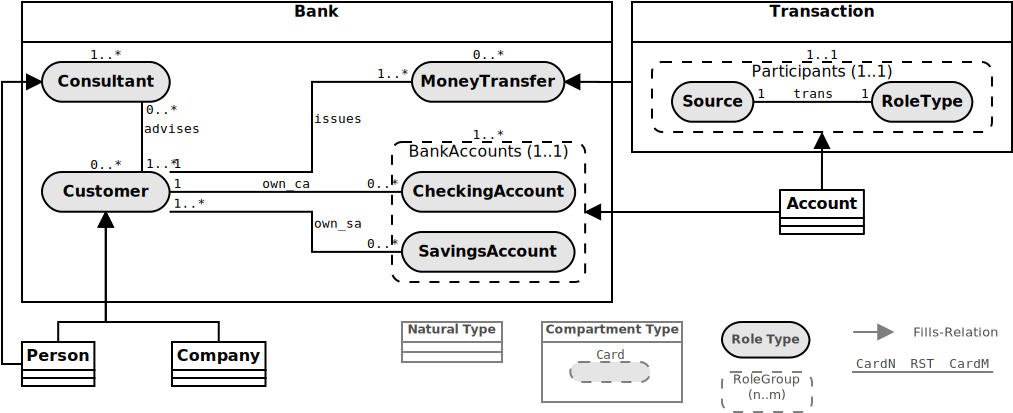
\includegraphics[width=\textwidth]{Bank-full-constraints}
  \caption{Graphical notation of a CROM for an banking application}
  \label{fig:bank}
\end{figure}

In our definitions, we omit to precisely define the graphical notation as they are not relevant for
reasoning on CROMs and refer to~\cite{KBG-SLE15}.

Next, we introduce instances of role-based models. An instance is based on a non-empty domain,
where each element is of exactly one type, i.e.\ a natural type, a \rosirole type or a compartment
type. Objects playing \rosirole in a compartment are collected in a ternary relation \plays and the
relation of two \rosiroles via a relationship type in a compartment is stored in \links.


\begin{definition}[Compartment Role Object Instance, Satisfiability]\label{def:scroi}
  Let $\Sigma = (\NT, \RT,$ $\CT,\RST)$ be a vocabulary.  Then, a
  \emph{Compartment Role Object Instance \I over $\Sigma$ (\SCROI)} is a tuple
  $\I=(\Gamma^{\I},\type,\plays,\links)$, where
  \begin{itemize}
  \item $\Gamma^{\I}$ is a non-empty domain, and
  \item $\type:\Gamma^{\I}\to\NT\cup\RT\cup\CT$ is a total function.
  \end{itemize}
  Based on the \type-function, we can partition the domain into the set \Nsf of \emph{naturals},
  i.e.\ all instances of any natural type, the set \Rsf of \emph{\rosiroles}, i.e.\ all instances of
  any \rosirole type, and the set \Csf of \emph{compartments}, i.e.\ all instances of any
  compartment type. Furthermore, the set \Osf of \emph{objects} denote all domain elements that are
  eligible to play a \rosirole, i.e.\ all naturals and compartments.
  \begin{align*}
    \Nsf & \coloneqq \{d \in \Gamma^{\I} \mid \type(d) \in \NT\} \\
    \Rsf & \coloneqq \{d \in \Gamma^{\I} \mid \type(d) \in \RT\} \\
    \Csf & \coloneqq \{d \in \Gamma^{\I} \mid \type(d) \in \CT\} \\
    \Osf & \coloneqq \Nsf \cup \Csf
  \end{align*}
  %
  Now, \plays and \links are defined as follows:
  \begin{itemize}
  \item $\plays \subseteq \Osf\times\Csf\times\Rsf$ is a ternary relation, and
  \item $\links: (\RST\times\Csf) \to \powerset{\Rsf\times\Rsf}$ is a total function.
  \end{itemize}
  %
  Furthermore, %
  the set $T^{\I}$ of all elements of type $T\in(\NT\cup\RT\cup\CT)$, %
  the set \Osf[\I,c] of all objects playing a role in $c$, %
  the set \Osf[\I,c,\rt] of all objects playing an \rt-role in $c$, and %
  the set \Rsf[\I,c] of all roles played in $c$ %
  are defined as follows:
  \begin{align*}
    T^{\I}     & \coloneqq \{d \in \Gamma \mid \type(d) = T\},\\
    \Osf[\I,c] & \coloneqq \{o \in \Osf \mid \text{there is some $r$ with $(o,c,r) \in \plays$}\}, \text{ and}\\
    \Osf[\I,c,\rt] & \coloneqq \{o \in \Osf \mid \text{there is some $r$ with $(o,c,r) \in \plays$
                     and $r\in\rt^{\I}$}\}\\
    \Rsf[\I,c] & \coloneqq \{r \in \Rsf \mid \text{there is some $o$ with $(o,c,r) \in \plays$}\}.
  \end{align*}
  %
  A \SCROI{} \I \emph{satisfies} a \SCROM{} \Mmc, denoted by $\I\models\Mmc$, if it has the following
  properties:
  \begin{enumerate}
  \item The \plays-relation respects \fills, i.e.~for each tuple $(o,c,r)\in\plays$ the type of $o$
    fills the type of $r$:
    \begin{align*}
      \{(o,r)\mid(o,\cdot,r)\in\plays\}\ \subseteq\ \{(o,r)\mid\text{there exists
        $(T,\rt)\in\fills$ s.t. $o\in T^{\I}$, $r\in \rt^{\I}$}\}.
    \end{align*}
  \item The \plays-relation respects \parts, i.e.~for each tuple $(o,c,r)\in\plays$ the type of $r$
    participates in the type of $c$:
    \begin{align*}
      & \{(c,r)\mid(\cdot,c,r)\in\plays\}\\
      & \quad \subseteq\ \{(c,r)\mid \text{there exists $\ct \in \CT$, $\rt \in \RT$ s.t. $c \in
        \ct^{\I}$, $r \in \rt^{\I}$, $\rt \in \parts(\ct)$}\}.
    \end{align*}
  \item Each object can only play one role of each role type in each compartment:
    \begin{align*}
      \{(o,c,r),(o,c,r')\}\subseteq\plays \textImplies \type(r)\neq\type(r').
    \end{align*}
  \item Each role is played by exactly one object in exactly one compartment:
    \begin{align*}
      |\{(o,c)\mid(o,c,r)\in\plays\}| = 1 \quad\text{for all $r \in \Rsf$}.
    \end{align*}
  \item Roles occurring in the image of \links are played in the associated compartment, i.e.\ for
    each $(r_{1},r_{2})\in\links(\rst,c)$ there exists objects that play $r_{1}$ and $r_{2}$ in $c$:
    \begin{align*}
      \{r_{1} \mid (r_{1},\cdot) \in \links(\cdot,c)\} \cup \{r_{2} \mid (\cdot,r_{2}) \in \links(\cdot,c)\} \ \subseteq\ \{r\mid(\cdot,c,r)\in\plays\}.
    \end{align*}
  \item The \links-function respects \rel, i.e.\ for each $(r_{1}, r_{2}) \in \links(\rst, \cdot)$ the
    types of $r_{1}$ and $r_{2}$ are related via \rst:
    \begin{align*}
      (r_{1},r_{2}) \in \links(\rst, \cdot) \textImplies \rel(\rst)=(\type(r_{1}),\type(r_{2})).
    \end{align*}
  \end{enumerate}

  A \SCROM{} \Mmc is \emph{satisfiable} if there exists any \SCROI{} \I such that $\I\models\Mmc$. 
\end{definition}

We say that $r$ is an $\rt$-role and $c$ is a $\ct$-compartment if, respectively,
$\type(r) = \rt \in \RT$ and $\type(c) = \ct \in \CT$.  Furthermore, \emph{$o$ plays $r$ in $c$} and
$o$ is the \emph{player} of $r$ if $(o,c,r) \in \plays$, and \emph{$r_{1}$ is linked to $r_{2}$ via
  $\rst$ in $c$} if $(r_{1}, r_{2}) \in \links(\rst, c)$.

% Again, it is easy to verify that our definition of a \SCROI satisfying a \SCROM is equivalent to the
% definition of~\cite{KBG-SLE15}.
% Since the \plays-relation respects the \fills- and the \parts-relation, if $o$ plays an \rt-role in
% a \ct-compartment, then the type of $o$ must fill \rt and \rt must participate in \ct. If $o$ plays
% $r_{1}$ and $r_{2}$ in $c$ then $r_{1}$ and $r_{2}$ must have different types, because each object
% can only play one role of each type in the same compartment. Moreover, for each role there exists
% exactly one object that plays it and one compartment where it is played in. In contrast to the
% formalisation in~\cite{KBG-SLE15} we omit $\varepsilon$-roles, but roles that are linked via a
% relationship type are both played in the same compartment and must be instances of the correct types
% since \links respects \rel.  Thus, equations (6) to (11) of~\cite{KBG-SLE15} are satisfied.

Before we investigate how the information about a \SCROM can be encoded in a description logic
ontology, we have to discuss the main reasoning tasks for role-based models. The arguably most
apparent question is, given a \SCROM{} \Mmc and a \SCROI{} \I, whether \I is compliant with
\Mmc. But as this task rather belongs to the area of model checking, we will not focus on that
problem in this thesis.
%
Instead, given a \SCROM{} \Mmc, it ismore interesting whether there exists any \SCROI that is
compliant with \Mmc.  Additionally, we often want to know for a specific \SCROM{} \Mmc whether there
exists a compliant \SCROI that fulfills certain assertions, e.g.\ that a role of a certain type is
played.  To express this assertional knowledge, we introduce a so-called \SCROA, a set of
assertions which should additionally be satisfied by a \SCROI.

\begin{definition}[$\Sigma$-Compartment Role Object Assertions] \label{def:scroa} Let
  $\Sigma = (\NT, \RT, \CT, \RST)$ be a vocabulary and let \INDC and \IND be two non-empty, disjoint
  sets of meta and object individual names disjoint from $\Sigma$.  A \emph{Compartment Role Object
    Assertion over $\Sigma$} is of the form
  \begin{itemize}
  \item $T(c)$ with $T\in\CT$ and $c\in\INDC$ (\emph{meta type assertion}),
  \item $T(a,c)$ with $T \in \NT \cup \CT \cup \RT$, $a\in\IND$ and $c\in\INDC$ (\emph{object type assertion}),
  \item $\playass(a_{1}, c, a_{2})$ with $a_{1}, a_{2} \in \IND$ and $c\in\INDC$ (\emph{plays assertion}), or
  \item $\linkass(\rst, c, a_{1}, a_{2})$ with $\rst \in \RST$ and  $a_{1}, a_{2} \in \IND$ and
    $c\in\INDC$ (\emph{link assertion}). 
  \end{itemize}

  A \emph{set of Compartment Role Object Assertions \A over $\Sigma$ (\SCROA)} is a set of such
  assertions.
  %
  We extend the \SCROI{} \I to additionally map individual names to domain elements, e.g.\
  $a\in\IND$ and $c\in\INDC$ are
  mapped to a domain elements $a^{\I} \in \Gamma^{\I}$ and $c^{\I} \in \Gamma^{\I}$. A \SCROI{} \I \emph{satisfies an assertion
    $\alpha$}, denoted by $\I\models\alpha$, if the following conditions hold:
  \begin{itemize}
  \item if $\alpha = T(c)$, then $c^{\I} \in T^{\I}$,
  \item if $\alpha = T(a, c)$, then $a^{\I} \in T^{\I} \cap (\Osf\cup\Rsf[\I,c])$,
  \item if $\alpha = \playass(a_{1}, c, a_{2}, )$, then
    $(a_{1}^{\I}, c^{\I}, a_{2}^{\I}) \in \plays$, and
  \item if $\alpha = \linkass(\rst, c, a_{1}, a_{2})$, then there exist $r_{1}, r_{2} \in \Rsf$ with
    $(a_{1}, c, r_{1})\in\plays$, $(a_{2}, c, r_{2})\in\plays$ and
    $(r_{1}^{\I}, r_{2}^{\I}) \in \links(\rst, c^{\I})$.
  \end{itemize}

  A \SCROI{} \I \emph{satisfies \A}, denoted by $\I\models\A$ if it satisfies all assertions
  in \A.
\end{definition}

Note here that the link assertion asserts for two objects that they play roles which are related via
\rst, and not that the objects themselves are related.
%
Moreover, without any assertions there always exists a trivial CROI that satisfies \Mmc with the
singleton set $\Gamma = \{o\}$ where the type of $o$ is some natural type, and \plays and \links are
empty sets. Therefore, we introduce in the next section further constraints.


\subsection{Constraint Level}
\label{sec:constraint-level}

When modelling a domain of interest, not only the type of an object defines whether that object is
allowed to play a certain role. In~\cite{KBG-SLE15} additional constraints were introduced. These
can be divided into four groups.

\emph{Role constraints} are the first category of constraints which state, for example, that roles
mutually exclude each other or playing one role implies playing another role. More general these
constraints are formalised with so-called \emph{role groups}. These consist of a set of role types
(or again role groups), a lower and an upper bound. An object fulfills a role group if it plays at
least the lower and at most the upper bound of roles from the set of role types.

\begin{definition}[Syntax of role groups]\label{def:syntax-role-groups}
  Let \RT be a set of role types. The set of \emph{role groups over \RT} is the smallest such that
  \begin{itemize}
  \item if $\rt \in \RT$, then \rt is an (\emph{atomic}) role group, and
  \item if $A_{1}$, \dots, $A_{n}$ are role groups, $k,\ell \in \nat$, then $(\{A_{1}, \dots, A_{n}\},
    k,\ell)$ is a (\emph{complex}) role group.
  \end{itemize}
  \emph{Atoms} of a role group $A$ are defined as:
  \begin{align*}
    \atom(A) & \coloneqq
               \begin{cases}
                 \{\rt\} & \text{if $A = \rt \in \RT$}\\
                 \bigcup_{i=1}^{n} \atom(A_{i}) & \text{if $A = (\{A_{1}, \dots, A_{n}\},k,\ell)$}.
               \end{cases}
  \end{align*}
  Role groups that occur within other role groups are called \emph{nested}.
\end{definition}

The semantics of a role group are based on a \SCROI and are locally evaluated for each domain
element and each compartment.  The interpretation function $\cdot^{\I,c,o}$ calculates recursively
whether an object fulfills the role group.

\begin{definition}[Semantics of role groups]\label{def:semantics-role-groups}
  Given a \SCROI{} \I, the semantics of a role group~$A$ is defined for an object $o \in \Osf$ in
  $c \in \Csf$ as follows:
  \begin{align*}
    A^{\I,c,o} & \coloneqq 
                 \begin{cases}
                   1 & \text{if $A = \rt\in\RT$ and $o$ plays an \rt-role in $c$, or} \\
                     & \text{if $A = (\{B_{1},\dots,B_{n}\},k,\ell)$ and $k \leq \sum_{i=1}^{k}
                     B_{i}^{\I,c,o} \leq \ell$, and}\\
                   0 & \text{otherwise.}
                 \end{cases}
  \end{align*}

  If $A^{\I,c,o} = 1$, we say that $o$ fulfills $A$ in $c$.
\end{definition}

\noindent
Basic role constraints, for example as defined in~\cite{RiGr-OOPLSLA98}, i.e.\ role implication,
role equivalence and role prohibition, can be expressed with role groups as well as much more
complex ones. In fact, any propositional formula can be emulated with role groups.

\begin{proposition}
  Let $\varphi$ be some propositional formula. Then, there exists a role group $A_{\varphi}$ such
  that $\varphi$ is satisfiable if and only if $A_{\varphi}$ can be fulfilled.
\end{proposition}
\begin{proof}
  We define $A_{\varphi}$ inductively as follows:
  
  \vspace{\topsep}
  \begin{tabular}{@{ if }l@{\quad then\quad }l}
    $\varphi = p$ & $A_{\varphi} \coloneqq \rt[p]$,\\
    $\varphi = \lnot \psi$ & $A_{\varphi} \coloneqq (\{A_{\psi}\}, 0, 0)$,\\
    $\varphi = \psi_{1}\land\psi_{2}$ & $A_{\varphi} \coloneqq (\{A_{\psi_{1}}, A_{\psi_{2}}\}, 2, 2)$, and\\
    $\varphi = \psi_{1}\lor\psi_{2}$ & $A_{\varphi} \coloneqq (\{A_{\psi_{1}}, A_{\psi_{2}}\}, 1, 2)$.
  \end{tabular}
  \vspace{\topsep}
  
  \noindent
  Next, we establish a 1-to-1-relation between a valuation $\rho$ for $\varphi$ and a
  $\Sigma$-CROI{} \I. For every propositional variable $P_{i}$ occurring in $\varphi$, we introduce
  a role type \rt[i] and assume that $o$ plays an \rt[i]-role iff $\rho(P_{i}) = \true$. By
  induction, it follows that $\rho(\varphi) = \true$ iff $o$ fulfills $A_{\varphi}$.
\end{proof}


The next category of constraints are \emph{occurrence constraints}. These state how often a role
type or role group must at least or at most be played in a compartment. Therefore, we introduce the
notion of a \emph{cardinality}, a pair $(k,\ell)\in\nat\times\natinf$ with $k\leq\ell$. We usually
denote cardinalities by $(k..\ell)$. Since role types are also atomic role groups, it suffices to
specify occurrence constraints for role groups.
%
Similar to multiplicities specified for associations in UML class diagrams, we specify
\emph{cardinality constraints} for relationship types. They express how often a role of certain type
must be related via a relationship type to some other role type.

Last but not least, the category of \emph{intra-relationship type constraints} imposes constraints on the
players of roles which are related via a relationship type. For example, stating that the
relationship type $\mathsf{isAncestorOf}$ between the role types $\mathsf{Parent}$ and
$\mathsf{Child}$ is transitive assures the existence of a respective link between a grandparent and
a grandchild. Note here, that the transitivity is evaluated over the players and not the roles
themselves.

\begin{definition}[Constraint set]
  Let $\Sigma = (\NT, \RT, \CT, \RST)$ be a vocabulary, let \RG be the set of role groups over \RT
  and let $\Card \coloneqq \nat \times \natinf$ be the set of cardinalities.  Then, a
  \emph{$\Sigma$-Compartment Role Object Constraint Set (\SCROC) \Cmc} is a tuple $\CC$ where
  \begin{itemize}[topsep=5pt]
  \item $\occur : \CT \to \powerset{\Card \times \RG}$,
  \item $\card : \RST \to \Card \times \Card$, and
  \item $\intra : \RST \to \powerset{\Emc}$ with \Emc being a set of functions of the form
    $e : \powerset{A\times B}\to \{\true, \false\}$ for arbitrary sets $A$, $B$.
  \end{itemize}
  are total functions.  The set of all non-nested role groups that appear in \occur is the set of
  \emph{top-level role groups \RG*}.
  %
  A \SCROC{} \Cmc is \emph{compliant} to a \SCROM if all atoms of a role group that is in the occurrence
  constraints of a compartment type participate in that compartment type. 
  %
  Before we define satisfiability, we introduce the following auxiliary functions:
  \begin{align*}
    \Succ(\rst,r,c) & \coloneqq \{r' \in \Rsf \mid (r,r') \in \links(\rst,c)\}, \\
    \Pred(\rst,r,c) & \coloneqq \{r' \in \Rsf \mid (r',r) \in \links(\rst,c)\}\text{, and} \\
    \links^{*}(\rst,c) & \coloneqq \{ (o_{1}, o_{2}) \mid (r_{1}, r_{2}) \in \links(\rst,c) \text{
                         and } (o_{1}, c, r_{1}), (o_{2}, c, r_{2}) \in \plays\}.
  \end{align*}
  %
  A \SCROI{} \I \emph{satisfies \Cmc}, denoted by $\I\models\Cmc$, if it has the following
  properties:
  \begin{enumerate}
  \item All occurrence constraints are respected, i.e.\ if $(k..\ell,A) \in \occur(\ct)$, then in
    every \ct-compartment there must exist at least~$k$ and at most~$\ell$ objects that fulfill role
    group~$A$:
    \begin{align*}
      ((k,\ell),A) \in \occur(\ct) \textImplies  \ct^{\I} \subseteq \left\{c \in \Csf \mmid k \leq \sum\nolimits_{o\in\Osf[\I,c]}
      A^{\I,c,o} \leq \ell \right\}
    \end{align*}
  \item All top-level \rosirole groups must be satisfied, i.e.\ if an object~$o$ plays an \rt-role and
    \rt is an atom of a top-level \rosirole group~A, then $o$ must fulfill~$A$:
    \begin{align*}
      & (o,c,r) \in \plays \text{, } r \in \rt^{\I} \text{ and } \rt \in \atom(A) \textImplies
      A^{\I,c,o} = 1\text{,} \\
      & \hspace{8cm} \text{for all $o \in \Osf$, $A \in \RG*$}.
    \end{align*}
  \item All cardinality constraints are respected, i.e.\ every \rosirole that is played in a
    compartment~$c$ and whose type is either the domain or the range of a relationship type~\rst
    with $\card(\rst) = (i..j, k..\ell)$ must have at least~$k$ and at most~$\ell$ \rst-successors
    in~$c$ or at least~$i$ and at most~$j$ \rst-predecessors in~$c$, respectively:
    \begin{align*}
      & (\cdot,c,r) \in \plays \text{, } r \in \rt[1]^{\I} \text{, } \rel(\rst) = (\rt[1], \cdot) \text{ and
        } \card(\rst)=(\cdot,k..\ell)\\
      & \qquad \textImplies k \leq | \Succ(\rst,r,c) | \leq \ell
    \end{align*}
    \begin{align*}
      & (\cdot,c,r) \in \plays \text{, } r \in \rt[2]^{\I} \text{, } \rel(\rst) = (\cdot, \rt[2]) \text{ and
        } \card(\rst)=(i..j,\cdot)\\
      & \qquad \textImplies i \leq | \Pred(\rst,r,c) | \leq j
    \end{align*}

  \item All intra-relationship type constraints are respected, i.e.\ every function $\fsf \in
    \intra(\rst)$, evaluated over the players of the roles related via \rst, must return \true:
    \begin{align*}
      & \fsf \in \intra(\rst) \textImplies \fsf(\links^{*}(\rst,c)) = \true \\
      & \qquad\text{for all $c$ in $\ct^{\I}$ s.t.\ \rst participates in \ct}.\qedhere
    \end{align*}
  \end{enumerate}
\end{definition}

The definition of satisfying a constraint model in~\cite{KBG-SLE15} is, neglecting
$\varepsilon$-roles, exactly reflected in the above definition. With constraints being formally
introduced, we can complete the CROM for the banking application of Example~\ref{ex:bank-crom} and Figure~\ref{fig:bank}.

\begin{example}
  We first define the complex \rosirole groups that occur in our example. The \rosirole group
  $\mathsf{Participants}$ in the context of an transaction ensures that a single account cannot be
  both the source and the target of an transaction. The \rosirole group $\mathsf{BankAccounts}$
  states the same for savings and checking accounts in the context of a bank. A single account
  cannot attain both \rosiroles simultaneously. 
  \begin{align*}
    \mathsf{Participants} & \coloneqq (\{\mathsf{Source}, \mathsf{Target}\},1,1)\\
    \mathsf{BankAccounts} & \coloneqq (\{\mathsf{SavingsAccount}, \mathsf{CheckingAccount}\},1,1)
  \end{align*}
  We next analyse the occurrence constraints. In our example a bank can only exists if it contains
  at least on consultant and one bank account. A transaction has exactly one source or
  target\footnote{Note here, that this small modelling error is made on purpose. We will discuss its
    logical implications later. Actually a transaction has exactly one source \emph{and} one target,
    and, hence, exactly two participants.}.
  \begin{align*}
    \occur(\mathsf{Bank}) & \coloneqq \{(1..\infty, \mathsf{Consultant}), (1..\infty, \mathsf{BankAccounts})\}\\
    \occur(\mathsf{Transaction}) & \coloneqq \{(1..1,\mathsf{Participants})\}
  \end{align*}
  For the appearing cardinality constraints we assume the following in the context of a bank. A
  consultant must advise at least one customer but not every customer necessarily needs a
  consultant. A customer does not need to have any bank account, but every bank account needs to
  have an owner. A checking account has exactly one owner, a savings account could have several. A
  money transfer is issued by exactly one customer and each customer issues at least one money
  transfer. In the context of a transaction, there is a one-to-one connection between source and
  target. 
  \begin{align*}
    \card(\mathsf{advises}) & \coloneqq (0..\infty,1..\infty)\\
    \card(\mathsf{own\_ca}) & \coloneqq (1..1,0..\infty)\\
    \card(\mathsf{own\_sa}) & \coloneqq (1..\infty,0..\infty)\\
    \card(\mathsf{issues}) & \coloneqq (1..1,1..\infty)\\
    \card(\mathsf{trans}) & \coloneqq (1..1,1..1)
  \end{align*}
  The intra-relationship type constraints are empty since we do not have such constraints in our
  example. 
\end{example}




At last we combine all parts of the role-based system into one \emph{constrained
  $\Sigma$-compartment Object Role Model}.

\begin{definition}[Constrained $\Sigma$-Compartment Role Object Model]
  \label{def:constrained-sigma-crom}
  Let $\Sigma = (\NT, \RT,$ $ \CT, \RST)$ be a vocabulary, let~\Mmc be a \SCROM, let~\Amc be a \SCROA
  and let~\Cmc be a \SCROC.
  %
  Then, a \emph{Constrained $\Sigma$-Compartment Role Object Model \SCCROM} is the tuple
  $\Kmc = (\Mmc, \Amc, \Cmc)$.

  The \emph{satisfiability problem} for \SCCROM{s} is the problem of deciding for a given \SCCROM{}
  $\Kmc = (\Mmc, \Amc, \Cmc)$ whether there exists a \SCROI that satisfies~\Mmc,~\Amc and~\Cmc.
\end{definition}



\section{Requirements for Logical Formalism}
\label{sec:requirements-and-CDLs}

Basically every large software project starts with modelling the application domain in UML. While
UML is the de facto standard as modelling language, it has several drawbacks. First of all, it has
no formally defined semantics~\cite{FrEL-CSI98}. While UML meta-models capture the precise syntax of
concepts used for modelling, they do little for answering questions of how to interpret non-trivial
UML diagrams.  For example, if one wants to map UML class diagrams to a logical formalism to be able
to reason about these diagrams, one takes certain assumptions about the intended meaning of the
occurring elements. Then a domain expert modelling some application has to trust that the logician
constructed the mapping with the same semantics in mind. Nevertheless, over the last years several
approaches for formal frameworks to reason on UML
arose~\cite{Eva-WIFT98,CaCG-ISMIS02,StMS-UML03,SiSJ-OBJ04,BeCG-AI05,SiBH-IJSEKE08,AhNa-ICET10}, from
which we can adapt some ideas, e.g. to model attributes of a~UML class with~DL roles and how
multiplicities of associations are modelled in~\cite{CaCG-ISMIS02}.

Besides that, UML lacks expressive power to model context-dependent domains. There also exist some
work on extending UML in that direction~\cite{ShB-ICMB05}, but here the semantics are even more ambiguous.
Therefore, we focus on role-based models that are based on CROM since it has both a well-defined,
formal semantics and the means to formulate the necessary concepts accordingly.

The only drawback might be the expressive restrictions of ``classical'' description logics as
explained in the introduction. Standard DLs cannot formalise contextual knowledge in a proper way
which is crucial for role-based systems.  In the recent years many different approaches and
extensions of DLs have been proposed~\cite{BoGH-ISWC03, BoGH-WS04, BeAF-ADVIS06, BaVS-ModOnt09, BaKP-JWS12,
  CePe-IJCAR14, CePe-JAR17}.  However, many were tailored to different goals, for example to support
context-specific reuse of ontologies or enable probabilistic reasoning. Additionally, these
approaches have a quite different intuition of what a context exactly is. In most cases it is simply
a finite set of names.  Serafini et al.~\cite{SeHo-JWS12} defines contexts by a set of
attribute-value declarations, one for each \emph{dimension}, e.g.\ time, topic or location to name a
few. There is only one context for each dimensional vector whereas there can exist many instances
of one compartment type.  Furthermore, except a coverage relation, one can hardly express any other
knowledge about the contexts such as the relational structure between them.  Hence, these
approaches seem not appropriate to model CROMs.

A far more promising formalism is the description logic of context \klarALC~\cite{KG-JELIA10, KG16}
mentioned in Section~\ref{sec:adding-cont-concepts}. Klarman et al.\ follow the ideas of McCarthy's
formalization of contexts~\cite{McC-ACM87,McC-IJCAI93} where contexts are formal objects, that have
properties and can be described, and that are organised in a relational structure.  This results in
a very expressive, two-dimensional description logic with strong interactions between the object and
the context level allowing to express information within a context that is valid in some other
context.  While transcending object knowledge through contexts is very important in the general
application of contextualised knowledge, it is complexity-wise very costly, especially in the
presence of rigid roles where the consistency problem becomes undecidable.

By restricting that interaction to a top-down view of contexts, we can retain decidability. From the
meta or context level, we can impose axioms that must hold within a certain context, but on the object
level, i.e.\ within a context, we cannot ``look outside''.
%
When formalizing compartments, this is exactly the needed expressiveness. For each compartment type
we want to specify the constraints which must hold within a compartment of that type.
%
This analysis led to the construction of \LMLO.
In Section~\ref{sec:adding-cont-concepts}, we showed that \ALCALC is indeed a sublogic of \klarALC.
We will now present how a CROM can be represented in \LMLO.


\section{Representing Role-Based Models}
\label{sec:representating-role-based-models}

We would like to emphasise here once again that checking well-formedness of a \SCROM{}~\Mmc and
compliance of a constraint set with \Mmc is not considered here, because these are purely
syntactical checks and no reasoning is necessary. Furthermore, checking whether a given \SCROI
satisfies \Mmc is also not the considered task as it rather belongs to the area of model checking
and is in the scope of this thesis. More interesting is whether there exists such a \SCROI at all.
Then, we can additionally test if certain axioms are entailed or whether specific role types can be
played since these questions can be reduced to the satisfiability problem. Thus, the main objective
is, given a \SCCROM{} \Kmc, to construct an \LMLO-ontology $\Bmf_{\Kmc}$ such that $\Bmf_{\Kmc}$ is
consistent iff \Kmc is satisfiable.

The general idea is to model compartment types as concepts on the meta level, and objects playing a
\rosirole, the relationship types as well as all the constraints within a compartment type on the
object level. For this, we introduce o-concepts for natural types and \rosirole types and a special
object role \plays. The fills relation is transformed into corresponding domain and range axioms for
\plays.

Here, we made a first design decision on how to express that a \rosirole is played within a
compartment. There are two possibilities, depicted in Figure~\ref{fig:two-ways-to-play-roles}, which
we already showed in Example~\ref{ex:nfl-with-contexts}. On the one hand, we can introduce
an o-concept $\mathsf{Coach}\in\RT$ and elements playing a $\mathsf{Coach}$-\rosirole are in the
extension of \rt (such as Mike McCarthy playing the \rosirole of a coach in the left side of
Figure~\ref{fig:two-ways-to-play-roles}). Here, an object $o$ and a \rosirole $r$ with
$(o,\cdot,r)\in\plays$ would be mapped to a single element $d$ in the object interpretation for that
compartment. This variant is close to the ontological nature of \rosiroles where an entity is in the
extension of a \rosirole, seen as unary predicate, if this entity plays that \rosirole. On the other
hand, we can introduce the o-concept $\mathsf{Coach}$ as well but disjoint from $\mathsf{Person}$
and we additionally introduce an object role \plays and elements playing an
$\mathsf{Coach}$-\rosirole have a \plays-successor that is in the extension of $\mathsf{Coach}$
(such as Mike playing the \rosirole of a coach in the left side of
Figure~\ref{fig:two-ways-to-play-roles}).  This is closer to the semantics of \SCROI{s}, but
introduces new object domain elements for each \rosirole that is played.  Still, we chose the latter
variant, since later we need to count the number of \rosiroles to assure occurrence and
cardinality constraints. In~DLs, this can be done via qualified number restrictions.

\begin{figure}
  \centering
  \begin{tikzpicture}
    \node[node,label={[align=left]270:\textit{MikeMcCarthy},\\ $\mathsf{Coach}$}] (mmc) at (-2,0){};
    \node[node,label={[align=left]270:\textit{MikeMcCarthy}}] (ar) at (2,0){};
    \node[node,label={[align=right]south:$\mathsf{Coach}$}] (qb) at (5,0){};
    \draw[edge] (ar) to[bend left=10] node{\plays} (qb);
    \draw[thin] (0,-1.5) to (0,1);
  \end{tikzpicture}
  \caption{Possibilities to formalise objects playing \rosiroles.}
  \label{fig:two-ways-to-play-roles}
\end{figure}

Generally, in a \SCROM, compartments are also allowed to play \rosiroles in other
compartments. Within these other compartments a compartment playing a \rosirole does not behave
differently than a natural. Hence, we have compartment types both as meta concept names, i.e.\ as
contexts in which other objects play \rosiroles, and as object concept types, i.e.\ as objects that
play \rosiroles in a context. In a \SCROM there is a one-to-one relationship, since the compartment
as \rosirole-player and as context is the same object. In our formalism, we cannot establish that
tight connection, but we can assure the existence of contexts of a certain compartment type via a
meta role \nested if objects of that type play \rosiroles. Since we cannot restrict the number of
existing contexts in a nested DL interpretation, this is sufficient for the satisfiability
problem. To distinguish between compartment types as contexts and as objects, we call the former
simply \emph{contexts} and the latter \emph{o-compartments} and introduce a copy \CT* of all
compartment types \CT.

Relationship types are intuitively modelled as object roles. Here, it might be more natural to span these
between the played \rosiroles instead of the players. But due to the one-to-one correspondence
between players and played \rosiroles, we can also construct the relationship types between the
players. In doing so, we can avoid the use of role value maps, which would cause the consistency
problem to become undecidable \cite{Sch89}, to formalise intra relationship type constraints. Even so, we
can only support such constraints that are expressible in the underlying DL.

\Rosirole groups are handled like \rosiroles with an additional axiom stating that ``playing'' a
\rosirole group is equivalent to fulfilling the constraints specified in that \rosirole
group. Furthermore, if an object plays an atom of a top-level \rosirole group, that object must
fulfill the \rosirole group.
%
For the occurrence constraints we introduce a fresh individual name \occurCounter and a object role
\counts and enforce that each played role or fulfilled role group is connected to this
counter. Thereby we can use qualified number restrictions to encode the occurrence constraints.
%
For cardinality constraints, we also utilise number restrictions.

% Ontologically, natural types would be captured as rigid concepts and their attributes, if present, as
% rigid roles, since that information does not change contexts-dependently. In our setting, rigidity
% has no influence on the consistency, and neglecting it decreases the computational complexity
% exponentially in the size of the input. Additionally, the case with rigid names can be handled quite
% similar and we come back to it in Section~\ref{sec:going-beyond-crom}.

To sum up, we consider the object signature $\Osig=(\OC,\OR,\OI)$ and the meta signature
$\Msig=(\MC,\MR,\MI)$ such that
\begin{itemize}
\item $\CT \subseteq \MC$, since every compartment type is a meta concept,
\item $\nested \in \MR$, to assure the existence of compartments that play \rosiroles,
\item $\NT\cup\CT* \subseteq \OCR$, since every natural type and every o-compartment type are rigid
  object concepts,
\item $\RT\subseteq\OCF$, since every \rosirole type is a flexible object concept
\item $\plays\in\ORF$, to express the \plays-relation, 
\item $\RST \subseteq \ORF$, since every relationship type is an object role,
\item $\occurCounter \in \OI$ and $\counts\in\ORF$, to express the occurrence constraints, and
\item $\INDC\in\MI$ and $\IND\in\OI$, to interpret individual names on their respective level. 
\end{itemize}
Additionally, we introduce the following object concept names:
\begin{itemize}
\item $\Ant\in\OCR$ for all objects eligible of playing \rosiroles, i.e.\ naturals and
  o-compartments,
\item $\Art\in\OCF$ for all \rosiroles, and
\item $\Arg\in\OCF$ for all instances of \rosirole groups since we
will consider \rosirole groups of the constraint set similar to \rosiroles.
\end{itemize}



% Additionally, we introduce the rigid object concept $\Ant \in \OCR$ for all objects eligible of
% playing \rosiroles, i.e.\ naturals and o-compartments.  and the flexible object concepts
% $\Art\in\OCF$ for all \rosiroles and $\Arg\in\OCF$ for all instances of \rosirole groups since we
% will consider \rosirole groups of the constraint set similar to \rosiroles.

\subsection{A Mapping for the Vocabulary  \texorpdfstring{\ensureboldmath{\Sigma}}{Sigma}}

In the next sections, we present the mapping from \rosirole-based systems into contextualised
description logics in detail.  At first, we express general knowledge about occurring types which is
independent of the specific \SCROM.


\begin{enumerate}

\item Every context belongs to exactly one compartment type.
\begin{align}
  \top & \sqsubseteq \bigsqcup_{\ct\in\CT} \ct \label{eq:compartments-coverage}\\
  \ct[1] \sqcap \ct[2] & \sqsubseteq \bot 
      \text{\qquad\qquad for all $\ct[1], \ct[2] \in \CT$, $\ct[1]\neq\ct[2]$}\label{eq:compartments-disjoint}
\end{align}

\item In every context, every natural or o-compartment and every \rosirole belongs to exactly one type.
\begin{align}
  \top & \sqsubseteq \oax{ \Ant \equiv \bigsqcup_{\nt\in\NT}\nt \sqcup \bigsqcup_{\ct*\in\CT*}\ct*}\label{eq:naturals-coverage}\\
  \top & \sqsubseteq \oax{ \Art \equiv \bigsqcup\limits_{\rt\in\RT}\rt} \label{eq:roles-coverage}\\
  \top & \sqsubseteq \bigsqcap_{\substack{T_{1},\,T_{2}\in\NT\cup\CT*\cup\RT,\\ T_{1} \neq T_{2}}}
      \oax{T_{1} \sqcap T_{2} \sqsubseteq \bot} \label{eq:roles-disjoint}
\end{align}

\item On the object level, an element can either be a \rosirole, a natural or o-compartment, an
instance of a \rosirole group or the individual \occurCounter.
\begin{align}
  %\top & \sqsubseteq \oax{\top \sqsubseteq \Ant \sqcup \Art \sqcup \Arg \sqcup \{\occurCounter\}}\\
  \begin{split}
  \top & \sqsubseteq \oax{\Ant \sqcap \Art \sqsubseteq \bot} 
      \sqcap \oax{\Ant \sqcap \Arg \sqsubseteq \bot}
      \sqcap \oax{\Art \sqcap \Arg \sqsubseteq \bot} \\
    & \qquad \sqcap \oax{\lnot(\Ant \sqcup \Art \sqcup \Arg)(\occurCounter)}
  \end{split}\label{eq:obj-disjoint}
\end{align}

\item Every natural or o-compartment can play at most one \rt-\rosirole in each context and each
  \rosirole must be played by some object.
  \begin{align}
    \top & \sqsubseteq \bigsqcap_{\rt\in\RT} \oax{\Ant \sqsubseteq \atmost{1}{\plays}{\rt}}\label{eq:roletype-played-max-once} \\
    \top & \sqsubseteq \oax{\Art \sqsubseteq \atleast{1}{\plays^{-}}{\top} 
           \sqcap \atmost{1}{\plays^{-}}{\top}}\label{eq:role-is-played-exactly-once}
  \end{align}

\item We formalise a general domain and range restriction for \plays. Only naturals or
  o-compartments can play something, and only \rosiroles or instances of \rosirole groups can be
  played.
  \begin{align}
    \top & \sqsubseteq \oax{ \exists\plays.\top \sqsubseteq \Ant}\label{eq:plays-domain} \\
    \top & \sqsubseteq \oax{\top \sqsubseteq \forall\plays.(\Art\sqcup\Arg)}\label{eq:plays-range}
  \end{align}

\item Finally, if an o-compartment plays a \rosirole in some context, the o-compartment must also
  exist as context.
  \begin{align}
    \lnot\oax{\ct* \sqcap \exists\plays.\top\sqsubseteq\bot} 
    & \sqsubseteq \exists\nested.\ct
      \text{\hspace{3em} for all $\ct* \in \CT*$}\label{eq:nested-cts}
  \end{align}
\end{enumerate}

% \noindent
% In every context, every natural or o-compartment and every \rosirole belongs to exactly one type.
% \begin{align}
%   \top & \sqsubseteq \oax{ \Ant \equiv \bigsqcup_{\nt\in\NT}\nt \sqcup \bigsqcup_{\ct*\in\CT*}\ct*}\label{eq:naturals-coverage}\\
%   \top & \sqsubseteq \oax{ \Art \equiv \bigsqcup\limits_{\rt\in\RT}\rt} \label{eq:roles-coverage}\\
%   \top & \sqsubseteq \bigsqcap_{\substack{T_{1},\,T_{2}\in\NT\cup\CT*\cup\RT,\\ T_{1} \neq T_{2}}}
%       \oax{T_{1} \sqcap T_{2} \sqsubseteq \bot} \label{eq:roles-disjoint}
% \end{align}

% \noindent
% On object level, an element can either be a \rosirole, a natural or o-compartment, an
% instance of a \rosirole group or the individual \occurCounter.
% \begin{align}
%   %\top & \sqsubseteq \oax{\top \sqsubseteq \Ant \sqcup \Art \sqcup \Arg \sqcup \{\occurCounter\}}\\
%   \begin{split}
%   \top & \sqsubseteq \oax{\Ant \sqcap \Art \sqsubseteq \bot} 
%       \sqcap \oax{\Ant \sqcap \Arg \sqsubseteq \bot}
%       \sqcap \oax{\Art \sqcap \Arg \sqsubseteq \bot} \\
%     & \qquad \sqcap \oax{\lnot(\Ant \sqcup \Art \sqcup \Arg)(\occurCounter)}
%   \end{split}\label{eq:obj-disjoint}
% \end{align}

% \noindent
% Next, every natural or o-compartment can only play one \rt-\rosirole in each context and
% each \rosirole must be played by some object.
% \begin{align}
%   \top & \sqsubseteq \bigsqcap_{\rt\in\RT} \oax{\Ant \sqsubseteq \atmost{1}{\plays}{\rt}}\label{eq:roletype-played-max-once} \\
%   \top & \sqsubseteq \oax{\Art \sqsubseteq \atleast{1}{\plays^{-}}{\top} 
%          \sqcap \atmost{1}{\plays^{-}}{\top}}\label{eq:role-is-played-exactly-once}
% \end{align}

% \noindent
% We formalise a general domain and range restriction for \plays. Only naturals or o-compart\-ments
% can play something, and only \rosiroles or instances of \rosirole groups can be played.
% \begin{align}
%   \top & \sqsubseteq \oax{ \exists\plays.\top \sqsubseteq \Ant}\label{eq:plays-domain} \\
%   \top & \sqsubseteq \oax{\top \sqsubseteq \forall\plays.(\Art\sqcup\Arg)}\label{eq:plays-range}
% \end{align}

% \noindent
% Finally, if an o-compartment plays a \rosirole in some context, the o-compartment must also exist as
% context.
% \begin{align}
%   \lnot\oax{\ct* \sqcap \exists\plays.\top\sqsubseteq\bot} & \sqsubseteq \exists\nested.\ct
%       \text{\hspace{3em} for all $\ct* \in \CT*$}\label{eq:nested-cts}
% \end{align}

\subsection{A Mapping for the \texorpdfstring{\SCROM{} \Mmc}{Sigma-CROM M}}

With the general knowledge about the vocabulary $\Sigma$ being set up, we can look into
the translation of the specifications for a given \SCROM{} \MM.

\begin{enumerate}
\item The \fills-relation specifies which natural or compartment types are allowed to play which \rosirole
types. Hence, elements that play a certain \rosirole type can only be naturals or o-compartments of
types which fill that \rosirole type.
\begin{align}
  \top & \sqsubseteq \bigsqcap_{\rt\in\RT}\oax{\exists\plays.\rt \sqsubseteq 
      \bigg( \bigsqcup\nolimits_{(T,\rt)\in\fills} T \bigg)} \label{eq:fills}
\end{align}
Note here, that Equation~\eqref{eq:fills} is sufficient in the sense that in conjunction with
Equations~\eqref{eq:roles-coverage} and~\eqref{eq:plays-range}, it entails that all \plays-successors
of naturals or o-compartments of a specific type are either instances of a \rosirole type that are
filled by that type or instances of a \rosirole group:
\begin{align*}
  \top & \sqsubseteq \bigsqcap_{T\in\NT\cup\CT*}\oax{T \sqsubseteq \forall\plays.
      \bigg(\Arg \sqcup \bigsqcup\nolimits_{(T,\rt)\in\fills} \rt \bigg)}.
\end{align*}

\item Since in a satisfying \SCROI the \plays-relation respects \parts, only \rt-\rosiroles with
$\rt\in\parts(\ct)$ exist in a \ct-context.
\begin{align}
  \ct & \sqsubseteq \oax{\Art \sqsubseteq \bigsqcup_{\rt\in\parts(\ct)}\rt}
      \text{\hspace{3em} for all $\ct\in\CT$} \label{eq:roles-in-compartment}
\end{align}

\item Analogous to \fills restricting the domain and range of \plays, the \rel-function
restricts them for each relationship type.
\begin{align}
  \begin{split}
    \top & \sqsubseteq \oax{\exists\rst.\top\sqsubseteq\exists\plays.\rt[1]} \sqcap
         \oax{\top\sqsubseteq\forall\rst.(\exists\plays.\rt[2])}\\
       & \hspace{7em}\text{for all $\rst\in\RST$ and $\rel(\rst) = (\rt[1],\rt[2])$}
  \end{split}\label{eq:rst-domain-range}
\end{align}
\end{enumerate}
% The \fills-relation specifies which natural or compartment types are allowed to play which \rosirole
% types. Hence, elements that play a certain \rosirole type can only be naturals or o-compartments of
% types which fill that \rosirole type.
% \begin{align}
%   \top & \sqsubseteq \bigsqcap_{\rt\in\RT}\oax{\exists\plays.\rt \sqsubseteq 
%       \bigg( \bigsqcup\nolimits_{(T,\rt)\in\fills} T \bigg)} \label{eq:fills}
% \end{align}
% Note here, that Equation~\eqref{eq:fills} is sufficient in the sense that in conjunction with
% Equations~\eqref{eq:roles-coverage} and~\eqref{eq:plays-range} it entails that all \plays-successors
% of naturals or o-compartments of a specific type are either instances of a \rosirole type that are
% filled by that type or instances of a \rosirole group.
% \begin{align*}
%   \top & \sqsubseteq \bigsqcap_{T\in\NT\cup\CT*}\oax{T \sqsubseteq \forall\plays.
%       \bigg(\Arg \sqcup \bigsqcup\nolimits_{(T,\rt)\in\fills} \rt \bigg)}.
% \end{align*}

% \noindent Since in a valid \SCROI the \plays-relation respects \parts, only \rt-\rosiroles with
% $\rt\in\parts(\ct)$ exist in a \ct-context.
% \begin{align}
%   \ct & \sqsubseteq \oax{\Art \sqsubseteq \bigsqcup_{\rt\in\parts(\ct)}\rt}
%       \text{\hspace{3em} for all $\ct\in\CT$} \label{eq:roles-in-compartment}
% \end{align}

% \noindent Analogous to \fills restricting the domain and range of \plays, the \rel-function
% restricts them for each relationship type.
% \begin{align}
%   \begin{split}
%     \top & \sqsubseteq \oax{\exists\rst.\top\sqsubseteq\exists\plays.\rt[1]} \sqcap
%          \oax{\top\sqsubseteq\forall\rst.(\exists\plays.\rt[2])}\\
%        & \hspace{7em}\text{for all $\rst\in\RST$ and $\rel(\rst) = (\rt[1],\rt[2])$}
%   \end{split}\label{eq:rst-domain-range}
% \end{align}

\noindent Note here, that due to equations~\eqref{eq:compartments-coverage},
\eqref{eq:roles-coverage},~\eqref{eq:roles-disjoint} and~\eqref{eq:roles-in-compartment} and the
fact that \parts' codomain is a partition of \RT, in any context that is not in \ct there are no
\rosiroles of a type the participates in \ct , e.g. the following axiom is entailed for all
$\ct\in\CT$:
\begin{align*}
  \lnot\ct & \sqsubseteq \oax{\bigsqcup_{\rt\in\parts(\ct)}\rt\sqsubseteq\bot}
\end{align*}

\subsection{A Mapping for the \texorpdfstring{\SCROA{} \A}{Sigma-CROA A}}

Next, let \A be a \SCROA. We can translate the different Compartment Role Object Assertions into
meta assertions in \LMLO.

\begin{enumerate}
\item For any meta type assertion of the form $\ct(c)\in\A$ with $\ct\in\CT$ and $c\in\INDC$ the individual $a$ must be a context of
type \ct.
\begin{gather}
  \ct(c)\label{eq:meta-type-assertion}
\end{gather}

\item For any object type assertion $T(a,c)\in\A$ with $T\in\NT\cup\CT\cup\RT$, $a\in\IND$ and $c\in\INDC$ the individual
$a$ is a natural, an o-compartment or \rosirole
  that belongs to the concept $T$ in context $c$.
\begin{gather}
  \oax{T(a)}(c)\label{eq:obj-type-assertion}
\end{gather}

\item A \plays assertion $\playass(a_{1}, c, a_{2}) \in \A$ states that $a_{1}$ plays $a_{2}$
  in $c$.
\begin{gather}
  \oax{\plays(a_{1},a_{2})}(c)\label{eq:plays-assertion}
\end{gather}

\item A \links assertion $\linkass(\rst, c, a_{1}, a_{2}) \in \A$ states that $a_{1}$ and $a_{2}$ play
\rosiroles which are related in $c$ via \rst. Due to the way we modelled relationship types, this is
simply the following axiom: 
\begin{gather}
  \oax{\rst(a_{1}, a_{2})}(c)\label{eq:links-assertion} 
\end{gather}
\end{enumerate}

% For any meta type assertion of the form $\ct(c)\in\A$ with $\ct\in\CT$ and $c\in\INDC$ the individual $a$ must be a context of
% type \ct.
% \begin{gather}
%   \ct(c)\label{eq:meta-type-assertion}
% \end{gather}

% \noindent
% For any object type assertion $T(a,c)\in\A$ with $T\in\NT\cup\CT\cup\RT$, $a\in\IND$ and $c\in\INDC$ the individual
% $a$ is a natural, an o-compartment or \rosirole
%   that belongs to the concept $T$ in context $c$.
% \begin{gather}
%   \oax{T(a)}(c)\label{eq:obj-type-assertion}
% \end{gather}

% \noindent
% A \plays assertion $\playass(a_{1}, c, a_{2}) \in \A$ states that $a_{1}$ plays $a_{2}$
%   in $c$.
% \begin{gather}
%   \oax{\plays(a_{1},a_{2})}(c)\label{eq:plays-assertion}
% \end{gather}

% \noindent
% A \links assertion $\linkass(\rst, c, a_{1}, a_{2}) \in \A$ states that $a_{1}$ and $a_{2}$ play
% \rosiroles which are related in $c$ via \rst. Due to the way we modelled relationship types, this is
% simply the following axiom: 
% \begin{gather}
%   \oax{\rst(a_{1}, a_{2})}(c)\label{eq:links-assertion} 
% \end{gather}
% % This is slightly more complicated as we mapped the
% %   relationship types between the players:
% % \begin{gather}
% %   (\oax{\rst(o_{1}, o_{2})}\sqcap\oax{\plays(o_{1}, a_{1})}\sqcap\oax{\plays(o_{2},
% %     a_{2})})(c)\label{eq:links-assertion} 
% % \end{gather}
% %where w.l.o.g.\ $o_{1}, o_{2}\in\OI\setminus\IND$ are fresh individual names.

\subsection{A Mapping for the \texorpdfstring{\SCROC{} \Cmc}{Sigma-CROC C}}
\label{sec:mapping-constraints}


Let \Cmc be a \SCROC, let $\RG(\Cmc)$ denote the set of all complex \rosirole groups occurring in
\Cmc and let $\RG*(\Cmc) \subseteq \RG(\Cmc)$ denote the set of all complex top-level \rosirole
groups. 

\begin{enumerate}

\item Analogous to \rosiroles, \rosirole groups are disjoint, every instance of a \rosirole group
must be played by some object and every object can either fulfill or not fulfill a \rosirole group.
\begin{align}
  \top & \sqsubseteq \oax{ \Arg \equiv \bigsqcup_{\rg\in\RG(\Cmc)}\rg} 
      \sqcap \bigsqcap_{\substack{\rg[1],\,\rg[2]\in\RG(\Cmc),\\ \rg[1]\neq\rg[2]}} 
      \oax{\rg[1] \sqcap \rg[2] \sqsubseteq \bot}
      \label{eq:rolegroups-coverage-and-disjoint}\\
  \top & \sqsubseteq \oax{\Arg \sqsubseteq \atleast{1}{\plays^{-}}{\top} 
      \sqcap \atmost{1}{\plays^{-}}{\top}}\label{eq:rgs-exactly-one-inverse-plays} \\
  \top & \sqsubseteq \bigsqcap_{\rg\in\RG(\Cmc)} \oax{\Ant \sqsubseteq \atmost{1}{\plays}{\rg}}\label{eq:obj-plays-max-one-rg}
\end{align}

\item Complex \rosirole groups are treated like abstract \rosiroles. An object can ``play'' an instance of
a \rosirole group. This is equivalent to fulfilling that role group. So, the object must ``play''
the required number of containing \rosirole groups.
%
Furthermore, if an object plays a \rosirole whose type is an atom of a top-level \rosirole group,
the object must also fulfill that \rosirole group.
\begin{align}
  \top & \sqsubseteq \bigsqcap_{\substack{\rg\in\RG(\Cmc),\\\rg = (\{A_{1}, \dots, A_{n}\},k,\ell)}}
      \oaxl{\exists\plays.\rg \equiv }
  \begin{aligned}[t]
    & (\atleast{k}{\plays}{(A_{1} \sqcup \dots \sqcup A_{n})}) \\
    &  \quad \sqcap \oaxr{(\atmost{\ell}{\plays}{(A_{1} \sqcup \dots \sqcup A_{n})})}
  \end{aligned}\label{eq:rg-declaration}\\
  \top & \sqsubseteq \bigsqcap_{\rg\in\RG*(\Cmc)}
      \oax{\exists\plays.\bigg(\bigsqcup\nolimits_{\rt\in\atom(\rg)}\rt\bigg)\sqsubseteq \exists\plays.\rg}\label{eq:rg-must-play}
\end{align}

\item Since for the occurrence constraints we only consider objects that play any \rosirole in this
compartment, we assure that fulfilling a \rosirole group implies playing some \rosirole.
\begin{align}
  \top & \sqsubseteq \oax{\exists\plays.\Arg\sqsubseteq\exists\plays.\Art}\label{eq:rgplayer-plays-role}
\end{align}

\item To capture the occurrence constraints we use an object individual name \occurCounter and introduce
an \counts-role from that individual to all \rosiroles and \rosirole group instances. Thus, the
occurrence constraints can be enforced with the help of qualified number restrictions.
\begin{align}
  \top & \sqsubseteq \oax{\Art \sqcup \Arg \sqsubseteq \atleast{1}{\counts^{-}}{\{\occurCounter\}} 
      \sqcap \atmost{1}{\counts^{-}}{\{\occurCounter\}}}\label{eq:counts-decl}\\
  \begin{split}
    \ct & \sqsubseteq \oax{(\atleast{k}{\counts}{\rg})(\occurCounter)}
    \sqcap \oax{(\atmost{\ell}{\counts}{\rg})(\occurCounter)}\\
    & \text{\rlap{\hspace{5em} for all $(k..\ell,\rg)\in\occur(\ct)$, for all $\ct\in\CT$}}
  \end{split}\label{eq:occurrence-constraints}
\end{align}

\item Cardinality constraints restrict the number of \rosiroles that are related to \rosirole via a
relationship type. \Rosiroles whose type is the domain or range of a relationship type \rst for
which there exists a cardinality constraint must have the correct amount of \rst successors or
predecessors, respectively.

\begin{align}
  \top & \sqsubseteq \bigsqcap_{\substack{\rst\in\RST, \\ \rel(\rst) = (\rt[1], \rt[2]), \\
  \card(\rst) = (i..j, k..\ell)}}
  \begin{aligned}[t]
    & \oax{\exists\plays.\rt[1] \sqsubseteq \atleast{k}{\rst}{\top} \sqcap \atmost{\ell}{\rst}{\top}} \\
    & \qquad\qquad \sqcap \oax{\exists\plays.\rt[2] \sqsubseteq \atleast{i}{\rst^{-}}{\top} \sqcap \atmost{j}{\rst^{-}}{\top}}
  \end{aligned}
   \label{eq:last-equation}
\end{align}

\item As mentioned above, because we spanned the relationship types between the players and not between the
\rosiroles, we can model at least some of the intra-relationship type constraints, exactly those
that are expressible in the object logic. In \SHOIQ, these would be transitivity and symmetry. Thus,
we add the following role axioms to the object RBox \RO:
\begin{gather}
  \trans{\rst}  \text{\qquad for all $\transsf\in\intra(\rst)$}\label{eq:rbox-1}\\
  \rst \sqsubseteq \rst^{-} \text{\qquad for all $\symm\in\intra(\rst)$}\label{eq:rbox-2}
\end{gather}
where $\transsf$ and $\symm$ are functions that return $\true$ if and only if the binary relation,
respectively, is transitive or symmetric.  But it is important to note, due to the restriction that
only simple roles are allowed to appear in number restrictions, we cannot impose any cardinality
constraints on the relationship type \rst if \rst is supposed to be transitive.

\end{enumerate}
% Analogous to \rosiroles, \rosirole groups are disjoint, every instance of a \rosirole group
% must be played by some object and every object can either fulfill or not fulfill a \rosirole group.
% \begin{align}
%   \top & \sqsubseteq \oax{ \Arg \equiv \bigsqcup_{\rg\in\RG(\Cmc)}\rg} 
%       \sqcap \bigsqcap_{\substack{\rg[1],\,\rg[2]\in\RG(\Cmc),\\ \rg[1]\neq\rg[2]}} 
%       \oax{\rg[1] \sqcap \rg[2] \sqsubseteq \bot}
%       \label{eq:rolegroups-coverage-and-disjoint}\\
%   \top & \sqsubseteq \oax{\Arg \sqsubseteq \atleast{1}{\plays^{-}}{\top} 
%       \sqcap \atmost{1}{\plays^{-}}{\top}}\label{eq:rgs-exactly-one-inverse-plays} \\
%   \top & \sqsubseteq \bigsqcap_{\rg\in\RG(\Cmc)} \oax{\Ant \sqsubseteq \atmost{1}{\plays}{\rg}}\label{eq:obj-plays-max-one-rg}
% \end{align}

% \noindent
% Complex \rosirole groups are treated like abstract \rosiroles. An object can ``play'' an instance of
% a \rosirole group. This is equivalent to fulfilling that role group. So, the object must ``play''
% the required number of containing \rosirole groups.
% %
% Furthermore, if an object plays a \rosirole whose type is an atom of a top-level \rosirole group,
% the object must also fulfill that \rosirole group.
% \begin{align}
%   \top & \sqsubseteq \bigsqcap_{\substack{\rg\in\RG(\Cmc),\\\rg = (\{A_{1}, \dots, A_{n}\},k,\ell)}}
%       \oax{\exists\plays.\rg \equiv (\atleast{k}{\plays}{(A_{1} \sqcup \dots \sqcup A_{n})}) 
%       \sqcap (\atmost{\ell}{\plays}{(A_{1} \sqcup \dots \sqcup A_{n})})}\label{eq:rg-declaration}\\
%   \top & \sqsubseteq \bigsqcap_{\rg\in\RG*(\Cmc)}
%       \oax{\exists\plays.\bigg(\bigsqcup\nolimits_{\rt\in\atom(\rg)}\rt\bigg)\sqsubseteq \exists\plays.\rg}\label{eq:rg-must-play}
% \end{align}

% \noindent 
% Since for the occurrence constraints we only consider objects that play any \rosirole in this
% compartment, we assure that fulfilling a \rosirole group implies playing some \rosirole.
% \begin{align}
%   \top & \sqsubseteq \oax{\exists\plays.\Arg\sqsubseteq\exists\plays.\Art}\label{eq:rgplayer-plays-role}
% \end{align}

% \noindent
% To capture the occurrence constraints we use an object individual name \occurCounter and introduce
% an \counts-role from that individual to all \rosiroles and \rosirole group instances. Thus, the
% occurrence constraints can be enforced with the help of qualified number restrictions.
% \begin{align}
%   \top & \sqsubseteq \oax{\Art \sqcup \Arg \sqsubseteq \atleast{1}{\counts^{-}}{\{\occurCounter\}} 
%       \sqcap \atmost{1}{\counts^{-}}{\{\occurCounter\}}}\label{eq:counts-decl}\\
%   \begin{split}
%     \ct & \sqsubseteq \oax{(\atleast{k}{\counts}{\rg})(\occurCounter)}
%     \sqcap \oax{(\atmost{\ell}{\counts}{\rg})(\occurCounter)}\\
%     & \text{\rlap{\hspace{5em} for all $(k..\ell,\rg)\in\occur(\ct)$, for all $\ct\in\CT$}}
%   \end{split}\label{eq:occurrence-constraints}
% \end{align}

% \noindent Cardinality constraints restrict the number of \rosiroles that are related to \rosirole via a
% relationship type. \Rosiroles whose type is the domain or range of a relationship type \rst for
% which there exists a cardinality constraint must have the correct amount of \rst successors or
% predecessors, respectively.

% \begin{align}
%   \top & \sqsubseteq \bigsqcap_{\substack{\rst\in\RST, \\ \rel(\rst) = (\rt[1], \rt[2]), \\
%   \card(\rst) = (i..j, k..\ell)}}
%   \begin{aligned}[t]
%     & \oax{\exists\plays.\rt[1] \sqsubseteq \atleast{k}{\rst}{\top} \sqcap \atmost{\ell}{\rst}{\top}} \\
%     & \qquad\qquad \sqcap \oax{\exists\plays.\rt[2] \sqsubseteq \atleast{i}{\rst^{-}}{\top} \sqcap \atmost{j}{\rst^{-}}{\top}}
%   \end{aligned}
%    \label{eq:last-equation}
% \end{align}

% \noindent
% As mentioned above, because we spanned the relationship types between the players and not between the
% \rosiroles, we can model at least some of the intra-relationship type constraints, exactly those
% that are expressible in the object logic. In \SHOIQ, these would be transitivity and symmetry. Thus,
% we add the following role axioms to the object RBox \RO:
% \begin{gather}
%   \trans{\rst}  \text{\qquad for all $\transsf\in\intra(\rst)$}\label{eq:rbox-1}\\
%   \rst \sqsubseteq \rst^{-} \text{\qquad for all $\symm\in\intra(\rst)$}\label{eq:rbox-2}
% \end{gather}
% where $\transsf$ and $\symm$ are functions that return $\true$ if and only if the binary relation,
% respectively, is transitive or symmetric.  But it is important to note, due to the restriction that
% only simple roles are allowed to appear in number restrictions, we cannot impose any cardinality
% constraints on the relationship type \rst if \rst is supposed to be transitive.


Before we establish the desired relation between the CROM and the ontology, we do a short
analysis of the required expressiveness of the meta and the object logic. To state the disjoint union
axioms we need at least~\ALC. As we do not need anything more on the meta level, we can
fix~\LM to be~\ALC. On the object level, we need qualified number restrictions and inverse roles to
assure that every \rosirole is played exactly once. 
%Hence, the minimal object DL is \ALCIQ. 
If we have a single occurrence constraint, we have to add nominals. Transitivity axioms or role
hierarchies are only required if some intra-relationship type constraint specifies a transitive or
symmetric relationship type, respectively. Table~\ref{tab:required-dls} shows a summary of the required DLs.

\begin{table}
  \caption{Summary of required DLs for \LM and \LO}
  \label{tab:required-dls}  \centering
  \begin{tabularx}{0.8\linewidth}{lXl}
    \toprule
    \LO & minimal                                  & \ALCIQ\\
        & with occurrence constraints              & \ALCOIQ\\
        & with intra-relationship type constraints & \SHOIQ\\
    \midrule
    \LM & & \ALC\\
    \bottomrule
  \end{tabularx}
\end{table}

Given a \SCCROM{} \Kmc, we obtain the \ALCSHOIQ ontology
$\Bmf_{\Kmc} = (\Bmc_{\Kmc}, \emptyset,\RO)$ where~$\Bmc_{\Kmc}$ is the conjunction of all meta
axioms from~\eqref{eq:compartments-coverage} to~\eqref{eq:last-equation} and~\RO is the set of all
role axioms~\eqref{eq:rbox-1} and~\eqref{eq:rbox-2}.

\begin{theorem}
  Let $\Kmc = (\Mmc, \Amc, \Cmc)$ be a \SCCROM. Then, \Kmc is satisfiable iff $\Bmf_{\Kmc}$ is consistent.
\end{theorem}
\begin{proof}
  Assume that \Kmc is satisfiable and let \IK denote a \SCROI that satisfies \Mmc, \Amc and
  \Cmc.  We define the set
  $\Delta_{\RT,c}$ of all \rosiroles played in $c$,
  the set $\Delta_{\RG,c}$ of all \rosirole group instances fulfilled in $c$,  and the nested interpretation \JJ as follows:
  \begin{align*}
    \Delta_{\RT,c} & \coloneqq \{r\in\Rsf[\IK] \mid (\cdot,c,r) \in\plays\} \text{\qquad for all $c\in\Csf[\IK]$}\\
    \Delta_{\RG,c} & \coloneqq \{(x,c,y) \in \RG\times\Csf[\IK]\times\Osf[\IK] \mid x^{\IK,c,y}=1\} \text{\qquad for all $c\in\Csf[\IK]$}\\[1ex]
    \Cbb & \coloneqq \Csf[\IK] \\
    \ct^{\J} & \coloneqq \ct^{\IK} \text{\qquad for all $\ct\in\CT$} \\
    \nested^{\J} & \coloneqq \{(c,o) \mid o,c\in\Csf[\IK], (o,c,\cdot)\in\plays\} \\[1ex]
    \Delta^{\J} & \coloneqq \Nsf[\IK] \cup \Csf[\IK] \cup \Rsf[\IK] \cup \bigcup_{c\in\Csf[\IK]}\Delta_{\RG,c} \cup \{d_{\occurCounter}\}\\
    \nt^{\I_{c}} & \coloneqq \nt^{\IK} \text{\qquad for all $\nt\in\NT$} \\
    \ct*^{\I_{c}} & \coloneqq \ct^{\IK} \text{\qquad for all $\ct\in\CT$} \\
    \rt^{\I_{c}} & \coloneqq \rt^{\IK} \cap \Delta_{\RT,c} \text{\qquad for all $\rt\in\RT$} \\
    \rg^{\I_{c}} & \coloneqq \{(\rg,c,y) \mid \rg^{\IK,c,y}=1\} \text{\qquad for all $\rg\in\RG(\Cmc)$}\\
    \Art^{\I_{c}} & \coloneqq \Delta_{\RT,c}\\
    \Ant^{\I_{c}} & \coloneqq \Osf[\IK]\\
    \Arg^{\I_{c}} & \coloneqq \Delta_{\RG,c}\\
    \rst^{\I_{c}} & \coloneqq \{(o_{1},o_{2})\mid\text{ there are $r_{1}$, $r_{2}$ s.t.\
                    $(o_{1},c,r_{1}),(o_{2},c,r_{2})\in\plays$ and}\\
                   & \hspace{3cm}\text{$(r_{1},r_{2})\in\links(\rst,c)$}\}\\
    \plays^{\I_{c}} & \coloneqq \{(o,r) \mid (o,c,r)\in\plays\}\\
                   &\hspace{3cm} \cup \{(o,r{\kern-0.1em}g) \mid r{\kern-0.1em}g =
                     (x,c,o)\in\Delta_{\RG,c}\text{ with $x^{\IK,c,o}=1$}\}\\
    \counts^{\I_{c}} & \coloneqq \{(d_{\occurCounter},y) \mid y\in\Delta_{\RT,c}\cup\Delta_{\RG,c}\}\\
    \occurCounter^{\I_{c}} & \coloneqq d_{\occurCounter}\\
    c^{\J} & \coloneqq c^{\IK} \text{\qquad for $c\in\INDC$}\\
    a^{\I_{c}} & \coloneqq a^{\IK} \text{\qquad for $a\in\IND$}
  \end{align*}
  It is straight forward to show that \J is a model of $\Bmf_{\Kmc}$. Note, that \J respects the
  rigid names since all \nt, \ct*, \Ant and individual names are interpreted the same in every
  world~$c$.
  %
  Axioms~\eqref{eq:compartments-coverage},
  \eqref{eq:compartments-disjoint},
  \eqref{eq:naturals-coverage},
  \eqref{eq:roles-disjoint},
  \eqref{eq:obj-disjoint},
  \eqref{eq:plays-domain},
  \eqref{eq:plays-range},
  \eqref{eq:meta-type-assertion} to~\eqref{eq:obj-plays-max-one-rg},
  \eqref{eq:counts-decl}
  %
  are modelled by construction of \J. Since
  $\Delta_{\RT,c}\subseteq\bigcup_{\rt\in\RT}\rt^{\IK} = \Rsf[\IK]$, \J models \eqref{eq:roles-coverage}.
  %
  Axioms~\eqref{eq:roletype-played-max-once} and~\eqref{eq:role-is-played-exactly-once} are modelled due
  to 3. and 4. of Definition~\ref{def:scroi}. 
  %
  Assume that $c_{1}\in(\lnot\oax{\ct* \sqcap \exists\plays.\top\sqsubseteq\bot})^{\J}$. Hence,
  $\I_{c_{1}}\not\models\ct* \sqcap \exists\plays.\top\sqsubseteq\bot$. Thus, there exists
  $c_{2}\in(\ct* \sqcap \exists\plays.\top)^{\I_{c_{1}}}$. Therefore,
  $(c_{2},c_{1},\cdot)\in\plays$, $(c_{1},c_{2})\in\nested^{\J}$ and $c_{2}\in\ct^{\J}$. Overall, \J
  models Axiom~\eqref{eq:nested-cts}.
  %
  Since \plays respects \fills and \parts, and \links respects \rel, \eqref{eq:fills},
  \eqref{eq:roles-in-compartment} and \eqref{eq:rst-domain-range} are satisfied.
  %
  Axioms~\eqref{eq:rg-declaration} to~\eqref{eq:rgplayer-plays-role} are satisfied due to the
  semantics of \rosirole groups and the fact that all top-level \rosirole groups are satisfied.
  %
  \IK respecting occurrence and cardinality constraints ensures that \J
  models~\eqref{eq:occurrence-constraints} and~\eqref{eq:last-equation}. 
  %
  Finally, the respective intra-relationship constraints imply the satisfaction of \RO.
  
  Conversely, let \JJ denote a model of $\Bmc_{\Kmc}$. W.l.o.g. we can assume that all
  o-compartments that exist also play some \rosiroles. Otherwise we could simply delete them, and
  still have a model. 
  %
  Let $\Delta_{\NT}\subseteq\Delta^{\J}$ and $\Delta_{\CT}\subseteq\Delta^{\J}$ denote,
  respectively, the set of all naturals and the set of all o-compartments, i.e.
  \begin{align*}
    \Delta_{\NT} & \coloneqq \bigcup_{\nt\in\NT} \nt^{\I_{\hat{c}}} \text{, and}\\
    \Delta_{\CT} & \coloneqq \bigcup_{\ct*\in\CT*} \ct*^{\I_{\hat{c}}}
  \end{align*}
  for some $\hat{c}\in\Cbb$.
  %
  Due to \eqref{eq:nested-cts}, there exists a mapping $\mu: \Delta_{\NT}\cup\Delta_{\CT} \to \Delta_{\NT}\cup\Cbb$ which maps
  o-compartments to contexts of respective type, i.e.
  \begin{align*}
    \mu(o) \coloneqq
    \begin{cases}
      o & \text{if $o\in\Delta_{\NT}$, and} \\
      c \text{ such that $c\in\ct^{\J}$} & \text{if $o\in\ct*^{\I_{\hat{c}}}$}.
    \end{cases}
  \end{align*}
W.l.o.g, we can assume that there exist
  sufficiently many contexts $c\in\Cbb$ to assure that $\mu$ preserves the occurrence and
  cardinality constraints, since we could introduce copies of $c$ if necessary.  We define the
  \SCROI{} \I as follows:
  \begin{align*}
    \Gamma^{\I} & \coloneqq \Cbb^{\J} \cup \Delta_{\NT} \cup \bigcup_{c\in\Cbb} \Art^{\I_{c}}\\
    \type(d) & \coloneqq  
               \begin{cases}
                 T & \text{if $T\in\CT$ and $d\in T^{\J}$}\\
                 T & \text{if $T\in\NT\cup\RT$ and $d\in T^{\I_{c}}$ for some $c$}
               \end{cases}\\
    (\mu(o),c,r) \in \plays & \text{\quad iff \quad $(o,r)\in\plays^{\I_{c}}$}\\
    (r_{1}, r_{2}) \in \links(\rst,c) & \text{\quad iff \quad $(o_{1},r_{1}), (o_{2},r_{2}) \in
                                        \plays^{\I_{c}}$ and $(o_{1}, o_{2})\in\rst^{\I_{c}}$}
  \end{align*}
  \I is well-defined and analogous to above one can go through the axioms step by step and show that
  \I satisfies \Kmc, e.g.\ Axiom~\eqref{eq:roles-in-compartment} ensures that \plays respects \parts
  in \I.
\end{proof}

Let us consider once again Example~\ref{ex:bank-crom} and Figure~\ref{fig:bank} to analyse some
implications which can be drawn due to the mapping into description logics.

\begin{example}
  Instead of writing down all axioms of the respective ontology $\Omc_{\Bank}$, we will rather point
  out some interesting inferences. At first we have a look at the \Bank compartment type, the
  \rosirole group \BankAccounts, the relationship types \ownca and \ownsa and the \rosirole type
  \Customer.

  Omitting general axioms, e.g.\ stating that every role or rolegroup instance is played and
  connected to \occurCounter, the following axioms are contained in the ontology, among others:
  \begin{align}
    % \top & \sqsubseteq \oax{\BankAccounts\sqsubseteq\exact{1}{\plays^{-}}{\top}}\\
    \Bank & \sqsubseteq \oax{(\atleast{1}{\counts}{\BankAccounts})(\occurCounter)}\label{eq:counter-bankaccount}\\
    \begin{split}
      \top & \sqsubseteq \oaxl{\exists\plays.\BankAccounts \equiv \atleast{1}{\plays}{(\CheckingAccount\sqcup\SavingsAccount)}}\\
      & \qquad\qquad \sqcap \oaxr{\atmost{1}{\plays}{(\CheckingAccount\sqcup\SavingsAccount)}}
    \end{split}\label{eq:decl-rg-bankaccounts}\\
    \top & \sqsubseteq \oax{\SavingsAccount\sqsubseteq\atleast{1}{\ownsa^{-}}{\top}}\label{eq:card-ownsa}\\
    \top & \sqsubseteq \oax{\CheckingAccount\sqsubseteq\atleast{1}{\ownca^{-}}{\top}}\label{eq:card-ownca}\\
    \top & \sqsubseteq \oax{\exists\ownsa.\top\sqsubseteq\Customer}\label{eq:domain-ownsa}\\
    \top & \sqsubseteq \oax{\exists\ownca.\top\sqsubseteq\Customer}\label{eq:domain-ownca}
  \end{align}
  In any interpretation \J that satisfies $\Omc_{\Bank}$ with $c\in\Bank^{\J}$,
  equations~\eqref{eq:counter-bankaccount} and~\eqref{eq:decl-rg-bankaccounts} entail the existence
  of an element in $\CheckingAccount^{\I_{c}}$ or $\SavingsAccount^{\I_{c}}$. Due to
  \eqref{eq:card-ownsa} and \eqref{eq:card-ownca}, there must be some element ``owning a CA or SA'',
  which must be in $\Customer^{\I_{c}}$ (\eqref{eq:domain-ownsa}
  and~\eqref{eq:domain-ownca}). Hence, the following axiom can be entailed:
\begin{align}
  \Bank & \sqsubseteq \oax{(\atleast{1}{\counts}{\Customer})(\occurCounter)},\label{eq:counter-customer}
\end{align}
stating that the occurrence constraint for \Customer is essentially $1..*$. For the
\Transaction compartment type we have:
\begin{align}
  \Transaction & \sqsubseteq \oax{(\atleast{1}{\counts}{\Participants} \sqcap
                 \atmost{1}{\counts}{\Participants})(\occurCounter)}\label{eq:counter-participants}\\
  \begin{split}
    \top & \sqsubseteq\oaxl{\exists\plays.\Participants \equiv
      \atleast{1}{\plays}{(\Source\sqcup\Target)}}\\
    & \qquad\qquad \sqcap \oaxr{\atmost{1}{\plays}{(\Source\sqcup\Target)}}
  \end{split}\label{eq:decl-rg-participants}\\
  \begin{split}
    \top & \sqsubseteq \oax{\Source \sqsubseteq \atleast{1}{\transBank}{\top} \sqcap
      \atmost{1}{\transBank}{\top}}\\
    & \qquad\qquad \sqcap \oax{\Target \sqsubseteq \atleast{1}{\transBank^{-}}{\top} \sqcap
      \atmost{1}{\transBank^{-}}{\top}} 
  \end{split}\label{eq:card-trans}\\
   \top & \sqsubseteq \oax{\exists\transBank.\top\sqsubseteq\Source} \sqcap \oax{\exists\transBank^{-}.\top\sqsubseteq\Target}\label{eq:domain-range-trans}
\end{align}
Assume that there would be some $d\in\Transaction^{\J}$.  By~\eqref{eq:counter-participants}
and~\eqref{eq:decl-rg-participants}, we know that there exists exactly one element in
$\Source^{\I_{d}}$ or $\Target^{\I_{d}}$. But due to~\eqref{eq:card-trans}
and~\eqref{eq:domain-range-trans}, there must also be an element in $\Target^{\I_{d}}$ or
$\Source^{\I_{d}}$, respectively. This results in two elements in $\Participants^{\I_{d}}$ which
contradicts~\eqref{eq:counter-participants}. Thus,
\begin{align}
  \Transaction & \sqsubseteq \bot\label{eq:transaction-bottom}
\end{align}
is entailed. Actually, the occurrence constraints for \Participants should be $2..2$.  Back to the
\Bank compartment, we also have
\begin{align}
  \top & \sqsubseteq \oax{\Customer\sqsubseteq\atleast{1}{\issues}{\top}}\label{eq:card-issues}\\
  \top & \sqsubseteq \oax{\exists\issues^{-}.\top\sqsubseteq\MoneyTransfer}\label{eq:range-issues}\\
  \top & \sqsubseteq \oax{\exists\plays.\MoneyTransfer\sqsubseteq\Transaction'}\label{eq:fills-moneytransfer}\\
  & \mathllap{\lnot}\oax{\Transaction'\sqcap\exists\plays.\top\sqsubseteq\bot} \sqsubseteq \exists\nested.\Transaction\label{eq:nested-transaction}
\end{align}
Due to~\eqref{eq:counter-customer},~\eqref{eq:card-issues} and~\eqref{eq:range-issues}, there must
be some element in $\MoneyTransfer^{\I_{c}}$ which must be $\mathsf{play}$ed by an element in
$\Transaction'^{\I_{c}}$. Thus, by~\eqref{eq:nested-transaction} we have to have some context
$c_{2}$ connected to $c$ via \nested with $c_{2}\in\Transaction$. But that
contradicts~\eqref{eq:transaction-bottom}.

Overall, the banking example is indeed inconsistent, due to a small modelling error in some
occurrence constraints within one compartment type that makes the whole domain model unsatisfiable.
\end{example}


Besides checking satisfiability in general, we can also address the following other questions a
domain analyst would be interested in:
\begin{enumerate}
\item[(Q1)] Is a specific compartment type \ct instantiable, i.e.\ does there exist some \SCROI{} \I
  s.t.\ $c \in \ct^{\I}$?
\item[(Q2)] Is the \rosirole type \rt playable, i.e.\ does there exist some \SCROI{} \I s.t. there is
  some $r \in \rt^{\I}$?
\item[(Q3)] Can two \rosiroles be linked via the relationship type \rst, i.e. does there exist some
  \SCROI{} \I s.t. there are some $r_{1}, r_{2}\in \Rsf$, $c\in \Csf$ with
  $\links(\rst,c)=(r_{1}, r_{2})$?
\item[(Q4)] Can more precise constraints be entailed, i.e.\ do there exist some cardinalities in \Cmc
  which can never be reached?
\item[(Q5)] Is some partial knowledge about an instance satisfiable, i.e.\ does there exist some
  \SCROI{} \I based this partial knowledge?
\end{enumerate}

To answer all these questions, we utilise \SCROA{s} as introduced earlier. For~(Q1), we add the meta
type assertion
\begin{gather*}
  \ct(a) 
\end{gather*}
to \A and check $\Bmf_{(\Mmc,\A,\Cmc)}$ for consistency. To answer~(Q2), an object type assertion of
the form
\begin{gather*}
  \rt(a,c), 
\end{gather*}
added to \A, is sufficient. W.l.o.g. we assume that $a$ and $c$ do not occur in
$\Bmf_{(\Mmc,\A,\Cmc)}$ before. Due to the other axioms already specified, the \rosirole must also
be played.
%
Similarly, for~(Q3) we add the link assertion
\begin{gather*}
  \linkass(\rst, c, a_{1}, a_{2}).
\end{gather*}
To test whether constraints are sharp, we assert the opposite and check for inconsistency. Here, we
will directly add axioms to $\Bmf_{(\Mmc,\A,\Cmc)}$. If, for example, there must exist at least $n$
roles of type \rt in \ct, we add
\begin{gather*}
  \ct \sqsubseteq \oax{(\atmost{n}{\counts}{\rt})(\occurCounter)} \land \ct(a)
\end{gather*}
to $\Bmf_{(\Mmc,\A,\Cmc)}$ which states that there must also exist at most $n$ \rt-roles. Then,
inconsistency of $\Bmf_{(\Mmc,\A,\Cmc)}$ would imply that there must indeed exist $n+1$ \rt-roles in
\ct.

For~Q5, we assume that we know certain facts about the domain. This could be the existence of a
compartment, a role or a link between two roles. These can all be formulated via a \SCROA, with
individual names adjusted accordingly.  If adding all respective assertions still preserves
consistency of $\Bmf_{(\Mmc,\A,\Cmc)}$, then there exists some \SCROI that satisfies \Mmc, \A and
\Cmc and respects these facts.


\section{Going beyond \texorpdfstring{$\Sigma$}{Sigma}-CROMs}
\label{sec:going-beyond-crom}

In~\cite{KuLG-SLE14}, Kühn et al. present a feature model for role-based modelling languages of
which the above defined CROM is one instance.  To support other variants of role-based models, the
same basic ideas of our mapping can be applied.  However, a detailed analysis which features can
easily be supported, is necessary.  The first feature that we will discuss is inheritance.

Let us assume, that additionally to a CROM we also have an irreflexive, asymmetric, functional
inheritance relation $\prec_{\nt}$ over the natural types. Inheritance is intuitively captured as a
GCI:
\begin{align}
  \label{eq:1}
  \top \sqsubseteq & \oax{\nt[a] \sqsubseteq \nt[b]} \text{ for all $\nt[a]\prec_{\nt}\nt[b]$}.
\end{align}
Then, obviously we have to adjust axiom~\eqref{eq:roles-disjoint} since natural types do not need to
be disjoint anymore. This implies that if some natural type \nt fills a role type \rt, then every
subtype of \nt also fills \rt.  Similarly, inheritance for compartment types could be handled.
Here, one has to make sure what exactly the intended semantics of compartment inheritance is
supposed to be. In our setting, a compartment subtype would be a specialization in the sense that
all axioms and constraints that hold for the supertype also hold for the subtype but there could
exist additional axioms or constraints in the subtype.

Some features in the feature model handle behaviour and dynamic aspects of role-based models. These
are not relevant in our case, as they have no influence on satisfiability. The same holds for
features about the ontological identity of roles and compartments.
%
All other features can easily be supported since only little changes to the mapping are required. These
include, among others, deep \rosiroles, i.e. \rosiroles which are allowed to play \rosiroles, or
whether a \rosirole type can be played several times by one object in the same compartment.


% \subsection{Adding Inheritance}
% \label{sec:adding-inheritance}

% Let us assume, that additionally to a CROM we also have an inheritance relation $\prec_{\nt}$ over
% the natural types.

% \todo[inline]{introduction paragraph}

% \todo[inline]{natural type inheritance - what is important in this setting}

% In the last sections we showed how contextualised description logics can represent \rosirole-based models

% \subsection{Further Features}
% \label{sec:further-constraints}


% \subsection{Going beyond CROM}
% \label{sec:temporal-aspects}

Two kinds of constraints that, in our opinion, might be important in practice, were not considered
until now: Constraints based on attributes of players and temporal constraints.

The first ones are quite easy to express in \LMLO. Besides some technical changes on the above
axioms, for each attribute $\mathsf{att_{i}}$ of a natural type or o-compartment, we introduce the
rigid role $\mathsf{att_{i}}\in\ORR$, since we assume that attributes of a rigid type are also
rigid.  Here, it might even be worth considering a description logic with concrete
domains~\cite{Lutz-PHD02,Lut-AiML02} as the object logic. We did not investigate these extensions of
DLs, but we conjecture that all results of Chapter~\ref{cha:context-dls} can be transferred without
much effort.

By utilising rigid types which are modelled with more detail, we can also introduce more fine-grained
constraints. For example, the \fills-relation could be specified to not only require a player of a
certain \rosirole type to be of some specific natural type but rather to demand that certain
attributes must exist. To be allowed to ``play'' the \rosirole of an employee, a person must have a
tax ID. Going a step further, we could also restrict \rosirole-playing based on the values of the
attributes. In the context of USA, a person can only play president if he is a ``natural born
citizen'' and at least 35 years old:
\begin{align*}
  \mathsf{USA} \sqsubseteq\oax{\exists\plays.\mathsf{President} \sqsubseteq \mathsf{Person} \sqcap
  \exists \mathsf{natural\_born\_citizen}.\{\true\} \sqcap \exists\mathsf{age \geq_{35}}}.
\end{align*}

Last but not least we can express additional complex constraints with arbitrary \LMLO axioms. For
example,
\begin{align*}
  \oax{\exists\rst.(\exists\rst.\top)\sqsubseteq\bot} \sqsubseteq \oax{\exists\rst.\top\sqsubseteq\bot}
\end{align*}
states that if there are no chains of length two for an relationship type \rst, then there will not
be any \rst at all in that particular compartment.


\cleardoublepage

%%% Local Variables:
%%% mode: latex
%%% TeX-master: "../thesis"
%%% reftex-default-bibliography: ("../references.bib")
%%% End:

%  LocalWords:  logics Kühn irreflexivity assertional satisfiability iff cardinalities CROM UML de
%  LocalWords:  facto ontologies DL nominals intra irreflexive GCI OntoClean metaproperties Bachman
%  LocalWords:  metaproperty unary


\chapter{JConHT -- A \texorpdfstring{\SHOIQSHOIQ}{SHOIQ[SHOIQ]} Reasoner}
\label{cha:jconht}

In the last chapter, we presented a mapping for role-based models into contextualised description
logic ontologies. This step can be automated which helps the automated processing and investigation
of role-based models. But to obtain a full automation we need a reasoner that is capable of handling
these ontologies, and can check the consistency automatically.

Since the translation for role-based models produces \LMLO-ontologies, i.e.\ conjunctions of meta
axioms, we will only consider \LMLO-ontologies. Throughout this chapter, let $\Omf=(\Omc,\RM,\RO)$
denote a \SHOIQSHOIQ-ontology and let \bsf denote the bijection as in
Definition~\ref{def:outer-abstraction}. Hence, \Ob denotes the outer abstraction of \Omc. We also
remind the reader that the \emph{restricted type} is the $\ran(\bsf)$-type (see
Definition~\ref{def:int-respects-D}) of some element and thus a subset of $\ran(b)$.

In this chapter, we present a practical algorithm to check consistency.  Furthermore, we implemented
this algorithm and give details on the design of the implementation.  Since internally, this
algorithm only calls standard DL consistency checks, we can reuse existing, highly optimized DL
reasoners.

\section{A Black-Box Approach}
\label{sec:blackbox-approach}

In Section~\ref{sec:complexity-consis-problem}, we showed that we can reduce the consistency problem
of \LMLO to two separate decision problems. Now, the general idea for an implementation is to use
performant reasoners as black-boxes for these subtasks.
%
In this section we discuss how the two subtasks, namely admissibility of a set~\Xmc and outer
consistency w.r.t.~\Xmc, can be reduced to standard reasoning tasks.


\subsection{Admissibility}
\label{sec:admissibility}

In the definition of admissibility (Definition~\ref{def:admissibility}), where we define $\Bmc_{X_{i}}$,
we require negated o-axioms. Negated axioms, especially negated GCIs, are usually not supported by
classical description logic reasoners. Therefore, we introduce the notion of \emph{weakly negated
  axioms}.

\begin{definition}[Weakly negated axioms]
  Let $\alpha$ be an axiom over \Nsig, then the \emph{weakly negated axiom $\alpha^{*}$} is defined
  as follows:
  \begin{itemize}
  \item if $\alpha = C \sqsubseteq D$, then $\alpha^{*} \coloneqq (C \sqcup \lnot D)(x)$ where $x$
    is a fresh variable,
  \item if $\alpha = C(a)$, then $\alpha^{*} \coloneqq (\lnot C)(a)$, and
%  \item if $\alpha = r(a,b)$, then $\alpha^{*} \coloneqq \lnot r(a,b)$, and
  \item for all other $\alpha$, $\alpha^{*} \coloneqq \lnot \alpha$. \qedhere
  \end{itemize}
\end{definition}

Note here, that for concept assertions the negation of the axiom $\lnot\alpha$ and weakly negated
axiom $\alpha^{*}$ are semantically equal, but not syntactical since $\lnot\alpha$ uses axiom
negation, while $\alpha^{*}$ only requires concept negation. Furthermore, in the presence of
nominals we could rewrite a negated role assertion of the form $\lnot r(a,b)$ as
$(\lnot\exists r.\{b\})(a)$. But as OWL reasoners in general support negated role assertions, we
keep $\lnot r(a,b)$.  Moreover, this definition reflects that $\alpha\land\alpha^{*}$ is
inconsistent, but not that $\I\models\alpha\lor\alpha^{*}$ for all interpretations \I.

\begin{lemma}\label{lem:weakly-negation-inconsistent}
  Let $\alpha$ be an axiom, and let \I be an interpretation. Then,
  \begin{enumerate}
  \item $\alpha\land\alpha^{*}$ is inconsistent, and
  \item if $\I\not\models\alpha$, then there exists an extension $\I'$ of $\I$ such that $\I'\models\alpha^{*}$.
  \end{enumerate}
\end{lemma}
\begin{proof}
  Let $\alpha = C \sqsubseteq D$ and $\alpha^{*} = (C \sqcup \lnot D)(x_{\mathsf{new}})$. Assume
  that $\I \models \alpha$ and $\I \models C(x_{\mathsf{new}})$.  Then, we know that
  ${x_{\mathsf{new}}}^{\I} \in C^{\I} \subseteq D^{\I}$. Thus we have
  ${x_{\mathsf{new}}}^{\I} \in D^{\I}$ and clearly
  ${x_{\mathsf{new}}}^{\I} \notin (C \sqcap \lnot D)^{\I}$. Hence,
  $C \sqsubseteq D \land (C \sqcap \lnot D)(x_{\mathsf{new}})$ is inconsistent.

  If $\I\not\models C \sqsubseteq D$, then there exists $d\in\Delta^{\I}$ such that
  $d \in C^{\I} \cap (\lnot D)^{\I}$. Then, the interpretation~$\I'$, obtained from \I by setting
  ${x_{\mathsf{new}}}^{\I'} \coloneqq d$, models $\alpha^{*}$.

  For the other axioms, the weakly negated axiom is defined as the normally negated axiom and the
  claim follows directly from the definition of $\models$ (see Definition
  \ref{def:semantics-of-axioms}).
\end{proof}

To check admissibility of a set of types, we distinguish whether or not rigid names are present. In
the latter case, i.e.\ $\OCR=\ORR=\emptyset$, the first condition of
Definition~\ref{def:admissibility} is always fulfilled. W.l.o.g., we can interpret the individual
names in the same way in every interpretation. Therefore, we can check each $\Bmf_{X_{i}}$ separately. We
show that it is sufficient to consider the weakly negated axioms.

% \begin{definition}[Sets of positive and negative induced o-axioms]
%   Let $\Xmc = \{X_{1}, \ldots, X_{k}\}$ be a set of restricted types. Then, the \emph{sets of
%     positive induced o-axioms $\Xposi$} are defined as
%   \begin{align*}
%     \Xposi & \coloneqq \{\alpha \mid \bsf(\oax{\alpha})\in X_{i}\}.\\
%   \intertext{The \emph{sets of negative induced o-axioms \Xnegi} are defined as}
%     \Xnegi & \coloneqq \{\alpha \mid \bsf(\oax{\alpha})\in\ran(\bsf)\setminus X_{i}\}.\qedhere
%   \end{align*}
% \end{definition}


\begin{lemma}\label{lem:admissibility-without-rigid}
  If no rigid names are present, i.e.\ $\OCR=\ORR=\emptyset$, the set $\Xmc = \{X_{1}, \ldots, X_{k}\}$ of restricted types is
  admissible iff $\Omf_{X_{i}} = (\Omc_{X_{i}}, \RO)$ is consistent for all $1 \leq i \leq k$, where
  $\Omc_{X_{i}}$ is defined as
  \begin{align*}
    \Omc_{X_{i}}:=\bigwedge_{\bsf(\oax{\alpha})\in X_{i}}\alpha\ \land \bigwedge_{\bsf(\oax{\alpha})\in\ran(\bsf)\setminus X_{i}}\alpha^{*}.
  \end{align*}
\end{lemma}
\begin{proof}
  Assume that \Xmc is admissible. Then there exists \Osig-interpretations
  $\I_1=(\Delta,\cdot^{\I_1})$,~\dots, $\I_k=(\Delta,\cdot^{\I_k})$ such that every $\I_i$,
  $1\le i\le k$, is a model of $\Bmf_{X_{i}}$ where $\Bmf_{X_{i}}$ is defined as in
  Definition~\ref{def:admissibility}. 
  Let \Xposi and \Xnegi respectively denote the sets of positive and negative induced o-axioms
  \begin{align*}
    \Xposi & \coloneqq \{\alpha \mid \bsf(\oax{\alpha})\in X_{i}\}\text{, and}\\
    \Xnegi & \coloneqq \{\alpha \mid \bsf(\oax{\alpha})\in\ran(\bsf)\setminus X_{i}\}.
  \end{align*}
  %
  By definition of \Xposi and \Xnegi, $\I_{i}$ is a model of
  $\smash{\bigwedge_{\alpha\in\Xposi}\alpha}$ and $\smash{\bigwedge_{\alpha\in\Xnegi}\lnot\alpha}$.
  %
  Now, let $\Xnegi=\{\alpha_{i,1}, \ldots, \alpha_{i,\ell_{i}}\}$. We have that
  $\I_{i}\models \lnot\alpha_{i,j}$ for $1 \leq j \leq \ell_{i}$. By Lemma
  \ref{lem:weakly-negation-inconsistent}, we get that there exists ${\I_{i}}'$ such that
  ${\I_{i}}'\models {\alpha_{i,j}}^{*}$. By induction, we get that ${\I_{i}}'\models\Omf_{X_{i}}$.

  If all $\Omf_{X_{i}}$ are consistent, there exist interpretations $\I_{i}$ such that
  $\I_{i}\models\Omf_{X_{i}}$. W.l.o.g., we can assume that the interpretations $\I_{i}$ share the same domain $\Delta$
  and that individual names are interpreted in the same way.  Then, $\I_{i}$ is a model of
  $\bigwedge_{\bsf(\oalpha)\in X_i}\alpha$,
  $\bigwedge_{\bsf(\oalpha)\in\ran(\bsf)\setminus X_i}\alpha^{*}$ and \RO. Due to Lemma
  \ref{lem:weakly-negation-inconsistent}, $\I_{i}$ also models
  $\bigwedge_{\bsf(\oalpha)\in\ran(\bsf)\setminus X_i}\lnot\alpha$. Hence, $\Xmc$ is admissible.
\end{proof}

In the former case, i.e.\ $\OCR\cup\ORR\neq\emptyset$, we use the renaming technique
of~\cite{BaGL-KR08,BaGL-ToCL12} as in the proof of
Theorem~\ref{thm:shoiqshoq-with-rigid-names-twoexptime}. Due to the interaction of the rigid names,
we must reason over all $\Bmf_{X_{i}}$ simultaneously.

\begin{definition}[Renamed axiom, sets of positive and negative induced renamed o-axioms, induced
  object ontology]\label{def:renaming}
  Let $\Xmc = \{X_{1}, \ldots, X_{k}\}$ be a set of restricted types and let $\alpha$ be an axiom
  over \Osig.
  %
  For $\iota\in\nat$, the \emph{renamed axiom $\alpha^{(\iota)}$} is obtained from $\alpha$
  by replacing all flexible concept names $A$, i.e.\ $A \in \OC \setminus \OCR$, with a copy $A^{(\iota)}$
  and all flexible role names $r$ with a copy $r^{(\iota)}$ where we assume w.l.o.g.\ that $A^{(\iota)}$ and
  $r^{(\iota)}$ do not occur in \Bmf.
  
  Then, the \emph{set of positively induced renamed o-axioms \Xpos}, the \emph{set of negatively induced
    renamed o-axioms \Xneg}, the \emph{renamed object RBox $\RO'$} and the \emph{induced object
    ontology $\Omf_{\Xmc}=(\Omc_{\Xmc},\RO')$} are defined as follows:
  \begin{align*}
    \Xpos & \coloneqq \smash{\bigcup_{i=1}^{k}}\vphantom{\bigcup_{i}}\{\alpha^{(i)} \mid \bsf(\oax{\alpha})\in X_{i}\},\\
    \Xneg & \coloneqq \bigcup_{i=1}^{k}\{\alpha^{(i)} \mid \bsf(\oax{\alpha})\in\ran(\bsf)\setminus X_{i}\},\\
    \RO' & \coloneqq \bigcup_{i=1}^{k}\{\alpha^{(i)} \mid \alpha\in\RO\} \text{, and}\\
    \Omc_{\Xmc} & \coloneqq \bigwedge_{\beta\in\Xpos} \beta\ \land\ \bigwedge_{\beta\in\Xneg}
                  \beta^{*}.
  \end{align*}

  \vspace{-1.7\baselineskip}
\end{definition}

Although the next lemma also holds if no rigid names are present, we state it explicitly with rigid
names, as in the other case we will use Lemma~\ref{lem:admissibility-without-rigid}. From now on,
let $\alpha$ always denote an original axiom and $\beta$ an renamed axiom.

\begin{lemma}\label{lem:admissibiliy-with-rigid}
  If rigid names are present, i.e.\ $\OCR\cup\ORR\neq\emptyset$, the set \Xmc of restricted types is
  admissible iff the induced object ontology $\Omf_{\Xmc}$ is consistent.
\end{lemma}
\begin{proof}
  We can reuse the claim made in the proof of
  Theorem~\ref{thm:shoiqshoq-with-rigid-names-twoexptime}: \Xmc is admissible iff $\Bmf_{\Xmc}$ is
  consistent where $\Bmf_{\Xmc}$ is defined as
  \begin{align*}
    \Bmf_\Xmc \coloneqq \left(\bigwedge\nolimits_{1\leq\iota\leq k}\left(\bigwedge_{\bsf(\oalpha)\in X_{\iota}}\alpha^{(\iota)}\ \land
      \bigwedge_{\bsf(\oalpha)\in\ran(\bsf)\setminus X_{\iota}}\lnot\alpha^{(\iota)}\right), \quad\RO'\right).
  \end{align*}
  %
  Hence, we only have to show that $\Bmf_{\Xmc}$ is consistent iff $\Omf_{\Xmc}$ is consistent. Let
  $\Xneg=\{\beta_{1}, \ldots, \beta_{\ell}\}$.

  If there exists an \Osig-interpretation \Gmc such that $\Gmc\models\Bmf_{\Xmc}$, then we also have
  that $\Gmc\models\lnot\beta_{i}$ for all $1 \leq i \leq \ell$. Due to
  Lemma~\ref{lem:weakly-negation-inconsistent} and by induction, there is some $\Gmc'$ such that
  $\Gmc'\models\beta_{i}^{*}$ for all $1 \leq i \leq \ell$. Hence, $\Gmc'$ is a model of $\Omf_{\Xmc}$.

  Conversely, if there exists an \Osig-interpretation \Gmc such that $\Gmc\models\Omf_{\Xmc}$, then we also have
  that $\Gmc\models\beta_{i}^{*}$ for all $1 \leq i \leq \ell$. By
  Lemma~\ref{lem:weakly-negation-inconsistent}, we know that $\Gmc\not\models\beta_{i}$. Hence,
  $\Gmc\models\lnot\beta_{i}$ and $\Gmc\models\Bmf_{\Xmc}$.
  


  % If $\Omc_{\Xmc}$ is consistent, then there exists an interpretation \II such that
  % $\I\models\Omc_{\Xmc}$. Let $\Xneg=\{\beta_{1}, \ldots, \beta_{l}\}$. We have that
  % $\I\models{\beta_{j}}^{*}$ for $1 \leq j \leq l$. By Lemma \ref{lem:weakly-negation-inconsistent}
  % we know that $\I\not\models\beta_{j}$ and, hence, $\I\models\lnot\beta_{j}$. By induction, we get
  % \begin{align*}
  %   \I \models & \left(\bigwedge_{\beta\in\Xpos} \beta\ \land\ \bigwedge_{\beta\in\Xneg} \lnot\beta,
  %   \quad\RO'  \right)
  % \end{align*}
  % We define \Osig-interpretations $\I_1=(\Delta,\cdot^{\I_1}), \ldots, \I_k=(\Delta,\cdot^{\I_k})$
  % as follows:
  % \begin{align*}
  %   \Delta & \coloneqq \Delta^{\I},\\
  %   A^{\I_{i}} & \coloneqq A^{\I} \qquad \text{for all $A\in\OCR$ occurring in \Xmc,}\\
  %   A^{\I_{i}} & \coloneqq (A^{(i)})^{\I} \qquad \text{for all $A\in\OC\setminus\OCR$ occurring in \Xmc,}\\
  %   r^{\I_{i}} & \coloneqq r^{\I} \qquad \text{for all $r\in\ORR$ occurring in \Xmc,}\\
  %   r^{\I_{i}} & \coloneqq (r^{(i)})^{\I} \qquad \text{for all $r\in\OR\setminus\ORR$ occurring in
  %                \Xmc, and}\\
  %   a^{\I_{i}} & \coloneqq a^{\I} \qquad \text{for all $a\in\OI$ occurring in \Xmc.}
  % \end{align*}
  % Condition (I) of Definition \ref{def:admissibility} is fulfilled since rigid names and individual
  % names are defined the same for all $\I_{i}$.
  % %
  % By the definition of $\I_{i}$, we have that $\I_{i}\models\alpha$ iff
  % $\I\models\alpha^{(i)}$. Hence, we know that $\I_{i}$ is a model of
  % $\bigwedge_{\bsf(\oax{\alpha})\in X_{i}}\alpha$,
  % $\bigwedge_{\bsf\oax{\alpha}\in\ran(\bsf)\setminus X_{i}}\lnot\alpha$ and \RO and \Xmc is
  % admissible.

  % If \Xmc is admissible, then there exist \Osig-interpretations $\I_1=(\Delta,\cdot^{\I_1})$,
  % \ldots, $\I_k=(\Delta,\cdot^{\I_k})$ such that $x^{\I_i}=x^{\I_j}$ for all
  % $x\in\OI\cup\OCR\cup\ORR$ and all $i,j\in\{1,\dots,k\}$, and every $\I_i$, $1\le i\le k$, is a
  % model of the \LO-BKB $\Bmf_{X_{i}}= (\B_{X_i},\RO)$ over~\Osig where
  % $\B_{X_i}:=\bigwedge_{\bsf(\oalpha)\in X_i}\alpha\ \land
  % \bigwedge_{\bsf(\oalpha)\in\ran(\bsf)\setminus X_i}\lnot\alpha$. We define the
  % \Osig-interpretation \II as follows:
  % \begin{align*}
  %   \Delta^{\I} & \coloneqq \Delta,\\
  %   A^{\I} & \coloneqq A^{\I_{i}} \qquad \text{for $A\in\OCR$ and some $1\leq i \leq k$,}\\
  %   (A^{(i)})^{\I} & \coloneqq A^{\I_{i}} \qquad \text{for $A\in\OC\setminus\OCR$,}\\
  %   r^{\I} & \coloneqq r^{\I_{i}} \qquad \text{for $r\in\ORR$ and some $1\leq i \leq k$,}\\
  %   (r^{(i)})^{\I} & \coloneqq r^{\I_{i}} \qquad \text{for $r\in\OR\setminus\ORR$, and}\\
  %   a^{\I} & \coloneqq a^{\I_{i}} \qquad \text{for $a\in\OI$ and some $1\leq i \leq k$.}\\
  % \end{align*}
  % Again, by definition of \I, we have that $\I\models\alpha^{(i)}$ iff $\I_{i}\models\alpha$. Thus, we
  % get that \I is a model of $\bigwedge_{\beta\in\Xpos} \beta$,
  % $\bigwedge_{\beta\in\Xneg} \lnot\beta$ and $\RO'$. Due to Lemma
  % \ref{lem:weakly-negation-inconsistent}, \I is also models $\bigwedge_{\beta\in\Xneg}
  % \beta^{*}$. Hence, $\Omc_{\Xmc}$ is consistent.
\end{proof}

To sum up, we can decide admissibility of~\Xmc by checking, respectively,~$\Omf_{\Xmc}$
or~$\Omf_{X_{i}}$ for consistency, depending on whether rigid names are present or not. 


\subsection{Outer consistency}
\label{sec:outer-consistency-to-standard-reasoning}

In the decision procedures described in Section~\ref{sec:complexity-consis-problem}, we always
construct the set \Xmc first, and then check whether \Bmfb is outer consistent w.r.t.~\Xmc. In the
general case with rigid names we enumerate all sets $\Xmc\subseteq\powerset{\ran(\bsf)}$. When only
rigid concept names and no rigid role names are present, we non-deterministically guess a set \Xmc.
For the case without rigid names we construct the largest possible set \Xmc that is admissible,
and argue that any \Bmfb that is outer consistent w.r.t.\ some admissible $\Xmc'$ is also outer
consistent w.r.t.~\Xmc. Hence, we only have to test outer consistency w.r.t.\ to \Xmc. But all these
techniques involve the possibly unnecessary, exponentially large construction of \Xmc.
%
Alternatively, we can also use the following lemma, which is a direct consequence of
Lemma~\ref{lem:admissible-and-outerConsistent}.

\begin{lemma}
  \label{lem:consistant-and-admissible-types}
  The \LMLO-BKB \Bmf is consistent iff there is an \Msig-interpretation \Hmc such that
  $\Hmc \models \Bmfb$ and $\Zmc_{\Hmc} = \{\mathsf{type}_{\ran(b)}^{\Hmc}(d) \mid d \in \Delta^{\Hmc}\}$
  is admissible.
\end{lemma}

\begin{proof}
  Let us assume that \Bmf is consistent.
  By Lemma~\ref{lem:admissible-and-outerConsistent}, we know that if \Bmf is consistent, then there exists
  an admissible set \Xmc such that \Bmfb is outer consistent w.r.t~\Xmc. By the definition of outer
  consistency, there exists an \Msig-interpretation \Hmc that models \Bmfb and weakly respects
  $(\ran(\bsf), \Xmc)$.  By definition, we have that $\Zmc_{\Hmc} \subseteq \Xmc$. Since every subset of an
  admissible set is also admissible, \Zmc is also admissible.

  For the `if' direction we assume that $\Hmc \models \Bmfb$ and that~\Zmc is admissible.
  If $\Hmc \models \Bmfb$, then~\Bmfb is outer consistent w.r.t~\Zmc. Since~\Zmc is admissible, we
  know, due to Lemma~\ref{lem:admissible-and-outerConsistent}, that \Bmf is consistent.
\end{proof}



Due to Lemma \ref{lem:consistant-and-admissible-types}, we do not need to construct the set \Xmc
first. We can also enumerate all models \Hmc of \Bmfb, and check for each \Hmc if the occurring
types are admissible. Of course, if there exist one model of \Bmfb, then there exists infinitely
many. But we only need to check those that are \emph{essentially different}, i.e.~those for which the set of
occurring restricted types differs.

\begin{definition}[Essentially equal interpretations]
  For an \Msig-interpretation \Hmc, the \emph{set of occurring, restricted types $\Zmc_{\Hmc}$} is defined as
  \begin{align*}
    \Zmc_{\Hmc} & \coloneqq \{\mathsf{type}_{\ran(b)}^{\Hmc}(d) \mid d \in \Delta^{\Hmc}\}.
  \end{align*}
  The two \Msig-interpretations $\Hmc_{1}$ and $\Hmc_{2}$ are \emph{essentially equal} if $\Zmc_{\Hmc_{1}} =
  \Zmc_{\Hmc_{2}}$.
\end{definition}

Using the results of Lemma \ref{lem:admissibility-without-rigid}, \ref{lem:admissibiliy-with-rigid}
and \ref{lem:consistant-and-admissible-types}, we can construct a simple algorithm, as depicted in
Algorithm~\ref{alg:1}. Here, $\Omc_{Z_{i}}$ and $\Omc_{\Zmc_{\Hmc}}$ are respectively defined as in
Lemma~\ref{lem:admissibility-without-rigid} and Definition~\ref{def:renaming}. We enumerate all
essentially equal models of \Bmfb and check for each model \Hmc whether $\Zmc_{\Hmc}$ is
admissible. Note that on the object level, only classical consistency checks are used. On the meta level,
the bare information about consistency is not sufficient, since we also need information about the
restricted types occurring in the model. Hence, we need a DL reasoner that constructs a model and,
if consistent, returns the set of occurring restricted types.


\IncMargin{1em}
\RestyleAlgo{ruled}
\begin{algorithm}[t]
  \SetAlgoVlined
  \setstretch{1.1}
  \DontPrintSemicolon
  \SetKwData{true}{true}
  \SetKwData{false}{false}
  \SetKwInOut{Input}{Input}
  \SetKwInOut{Output}{Output}
  %
  \Input{\LMLO-BKB \Bmf}
  \Output{\true if \Bmf is consistent, \false otherwise}
  \BlankLine
  $\Hmf \coloneqq \{\Hmc \mid \Hmc\models\Bmfb \text{, up to essential equality}\}$\;
  \For{$\Hmc \in \Hmf$}{
    $\Zmc_{\Hmc} \coloneqq \{\mathsf{type}_{\ran(b)}^{\Hmc}(d) \mid d \in \Delta^{\Hmc}\}$\;
    \eIf{\Bmf contains rigid names}{
      \If{($\Omc_{\Zmc_{\Hmc}}, \RO')$ is consistent}{
        \vspace{0.5ex}\Return{\true}
      }
    }{
      $\Zmc_{\Hmc} = \{Z_{1}, \dots, Z_{k}\}$\;
      \If{$(\Omc_{Z_{i}}, \RO)$ is consistent for all $1 \leq i \leq k$}{
        \vspace{0.5ex}\Return{\true}
      }
    }
  }
  \Return{false}
  \caption{Algorithm for checking consistency of \LMLO-BKB \Bmf}\label{alg:1}
\end{algorithm}

\begin{lemma}\label{lem:alg1-sound-complete-terminating}
  Algorithm~\ref{alg:1} is sound, complete, and terminating.
\end{lemma}
\begin{proof}
  The set of essential equal models is finite. Checking whether \Hmc is a model and checking whether
  $\Omf_{\Zmc_{\Hmc}}$ or $\Omf_{Z_{i}}$ is consistent, is decidable. Thus, Algorithm~\ref{alg:1}
  terminates.

  Let us assume that \Bmf is consistent. By Lemma~\ref{lem:consistant-and-admissible-types}, there
  exists a model~\Hmc of~\Bmfb such that~$\Zmc_{\Hmc}$ is admissible. W.l.o.g., we can assume that
  $\Hmc\in\Hmf$. 
  %
  % Then, there exists a model \J of \Bmf and, hence, there is a model $\Hmc\in\Hmf$ of \Bmfb such
  % that \Hmc and \Jb are essential equal. By Lemma~\ref{lem:consistant-and-admissible-types},
  % $\Zmc_{\Hmc}$ is admissible.
  % 
  Depending on whether rigid names are present, due to
  Lemma~\ref{lem:admissibility-without-rigid} and Lemma~\ref{lem:admissibiliy-with-rigid} Algorithm~\ref{alg:1} will successfully check that
  $\Omf_{Z_{i}}$, for all $1\leq i \leq k$, or $\Omf_{\Zmc_{\Hmc}}$ is consistent. Hence, it
  returns \true.

  Let us assume that the algorithm returns \true. Then, there is some $\Hmc\in\Hmf$ such that~$\Omf_{Z_{i}}$,
  for all $1\leq i \leq k$, or~$\Omf_{\Zmc_{\Hmc}}$ is consistent. By
  Lemma~\ref{lem:admissibility-without-rigid} and Lemma~\ref{lem:admissibiliy-with-rigid}, we know
  that $\Zmc_{\Hmc}$ is admissible. Lemma~\ref{lem:consistant-and-admissible-types} yields that \Bmf
  is consistent.
\end{proof}



\section{Contextual Hypertableau}
\label{sec:using-hypertableau}

We have to take several arguments into account in order to evaluate, which reasoner or decision
procedure we use as core reasoner to decide the two subtasks.
%
First of all as mentioned earlier, in addition to checking consistency on meta level, we also need
the set of occurring restricted types of a model. Hence, an reasoner that constructs a model is
necessary for enumerating the models of \Bmfb. As pointed out in~\cite{MaLHSP-ORE15}, there exist
three major approaches used in OWL reasoners: consequence-, model construction- and
rewriting-based. \emph{Consequence-based} approaches are classically employed for the entailment
problem in lightweight DLs such as \EL, while \emph{rewriting} approaches are usually used for
specific reasoning tasks, such as for query answering. \emph{Model construction-based} approaches
are utilized for expressive DLs, i.e.\ any extension of \ALC, and try to build a model based on the
knowledge base to check consistency. These include tableau and hypertableau techniques. Since we
also need the information about the restricted types of a model, we are looking for a model
construction-based reasoner.

Furthermore, by means of maintenance, we will use the same reasoner for the meta level and the
object level.
%
Since a dominant framework supporting OWL, the OWL API~\cite{HoB-SW11}, is implemented in Java, so is the
majority of the available reasoners. Therefore, we also use Java for our OWL-conformant reasoner and
implement the \textsf{OWLReasoner} interface of the OWL~API.

Last but not least, the performance of the reasoner in consistency checking is important for
us. Therefore, we take a look at the OWL Reasoner Evaluation Competition
Report~\cite{PaMGGS-SSWS15}, especially at the results of the discipline: \emph{OWL DL
  Consistency}. This discipline, among others, was won by Konclude~\cite{StLG-JWS14}, a
 hybrid reasoner that combines tableau calculus with a variant of consequence-based
saturation procedure. This hybrid approach, however, makes Konclude unsuitable in our
setting. Besides that, it is implemented in C++ and we focus on Java-based reasoners. The
next candidate is HermiT~\cite{GHM-JAR14}, a Java-implemented reasoner based on the hypertableau
calculus~\cite{MoSH-JAIR09}. Since it meets all our requirements, we use HermiT as core reasoner in
our implementation.

% \todo[inline]{hypertableau avoid unnecessary nondeterminism (or-branching)}

% \todo[inline]{Hermit computes premodels which can be extended to model of ontology. blocked individuals, same
% concept labels -> premodel has the same restricted type}

% \todo[inline]{different blocking strategies dependant on used dl. anywhere blocking, ancestor blocking, atomic
% single blocking, full single blocking, }

% \todo[inline]{full subset blocking could be problematic, but is not used in HermiT.}

Before we discuss the details of our algorithm, we present the relevant parts of the
hypertableau algorithm and refer the interested reader
to~\cite{MoSH-CADE07,MoSH-DL07,MoSH-JAIR09}. Like other tableau-based methods, the hypertableau
calculus tries to construct an abstraction of a model for a given ontology to check whether that
ontology is consistent. But in contrast to other tableau calculi, it operates on a set of
\emph{DL-clauses} and an ABox, instead of a TBox and an ABox.

\begin{definition}[DL-Clause~\cite{MoSH-JAIR09}]
  The concepts $\top$, $\bot$, and concepts of the form $A$ and $\lnot A$ for $A\in\MC$ are called
  \emph{literal concepts}. Let \MV be the set of variables disjoint from the set of individuals
  \MI. An \emph{atom} is an expression of the form $B(x)$, $(\atleast{n}{s}{B})(x)$, $r(x,y)$, or
  $x\approx y$, for $x,y\in\MV\cup\MI$, $B$ a literal concept, $r$ an atomic role, $s$ a role, and
  $n$ a positive integer. A \emph{DL-clause} is an expression of the form
  \begin{align*}
    U_{1} \land\dots\land U_{m} \to V_{1} \lor\dots\lor V_{n}
  \end{align*}
  where $U_{i}$ and $V_{j}$ are atoms, $m,n\geq0$. The conjunction $U_{1} \land\dots\land U_{m}$ is
  called the \emph{antecedent}, and the disjunction $V_{1} \lor\dots\lor V_{n}$ is called
  \emph{consequent}. The empty antecedent and the empty consequent are respectively written as $\top$
  and $\bot$.

  Let \HH be an \Msig-interpretation and let $\mu:\MV\to\Delta^{\Hmc}$ be a mapping from variables to
  domain elements. We define $\cdot^{\Hmc,\mu}$ as follows:
  \begin{align*}
    c^{\Hmc,\mu} & \coloneqq
      \begin{cases}
        c^{\Hmc} & \text{ if $c\in\MI$, and}\\
        \mu(c)  & \text{ if $c\in\MV$}.
      \end{cases}
  \end{align*}
  Satisfaction of an atom, DL-clause, and a set of DL-clauses \Cmc in \Hmc and $\mu$ is defined in
  Table~\ref{tab:satisfaction-clauses}. 
\end{definition} 
\begin{table}
  \caption{Satisfaction of DL-Clauses}
  \centering
  {\renewcommand{\arraystretch}{1.1}
  \begin{tabularx}{0.9\linewidth}{l@{\hskip 10pt iff\hskip 10pt}L}
    \toprule
    $\Hmc,\mu\models C(c)$ & $c^{\Hmc,\mu} \in C^{\Hmc}$\\
    $\Hmc,\mu\models r(c,d)$ & $(c^{\Hmc,\mu},d^{\Hmc,\mu}) \in r^{\Hmc}$ \\
    $\Hmc,\mu\models c\approx d$ &  $c^{\Hmc,\mu}=d^{\Hmc,\mu}$ \\
    $\Hmc,\mu\models\bigwedge_{i=1}^{m}U_{i}\to\bigvee_{j=1}^{n}V_{j}$ 
        & $\Hmc,\mu\models U_{i}$ for each $1\leq i\leq m$ implies \hspace{2cm} \hspace*{1cm}$\Hmc,\mu\models V_{j}$ for some
          $1\leq j\leq n$\\
    $\phantom{\Hmc,\mu}\mathllap{\Hmc}\models\bigwedge_{i=1}^{m}U_{i}\to\bigvee_{j=1}^{n}V_{j}$
        & $\Hmc,\mu\models\bigwedge_{i=1}^{m}U_{i}\to\bigvee_{j=1}^{n}V_{j}$ for all mappings
          $\mu$\\
    $\phantom{\Hmc,\mu}\mathllap{\Hmc}\models\Cmc$ 
        & $\phantom{\Hmc,\mu}\mathllap{\Hmc}\models\mathbf{r}$ for all $\mathbf{r}\in\Cmc$\\ \bottomrule
  \end{tabularx}}
  \label{tab:satisfaction-clauses}
\end{table}

In the hypertableau algorithm, a few preprocessing steps are necessary, namely \emph{elimination of
  transitivity axioms}, \emph{normalization} and \emph{clausification}. The clausification
translates a normalized DL ontology $\Omf = (\Omc, \Rmc)$ without transitivity axioms into a pair
\CA, where \Cmc is a set of DL-clauses and \A is an ABox, and \Omf and \CA are equisatisfiable.
Here, we omit further details of the preprocessing steps, but emphasise that the preprocessing not
only preserves satisfiability, but also satisfiability w.r.t.~essential equality.  Let \Kmc be the
input ontology and \CA the clausification after normalization. There exists a model \I of \Kmc iff
the exists a model \Hmc of \CA such that \I and \Hmc are essentially equal. Hence, it is sufficient
to consider the clausification of the outer abstraction of an \LMLO ontology.

As typical for tableau algorithms, the hypertableau calculus uses a blocking strategy to ensure
termination. Intuitively, in the construction of a model, a blocked individual is replaced by its
blocker. Thus, infinite models can be constructed. Here, it is important for us, that the blocked
individual and its blocker have the same restricted type. This holds for all blocking strategies
used in the hypertableau algorithm. For the sake of conciseness, we omit the specific blocking
strategy in our definition of the hypertableau algorithm and refer to~\cite{MoSH-JAIR09} for a
complete definition.

\begin{definition}[Hypertableau Algorithm~\cite{MoSH-JAIR09}]
  Given a set of named individual \MI, the set of \emph{root individuals \MO} is the smallest set
  such that $\MI\subseteq\MO$, and if $x\in\MO$, then $x.\langle r,B,i \rangle\in\MO$ for each role
  $r$, literal concept $B$ and positive integer $i$. The set of \emph{all individuals} \MA is the
  smallest set such that $\MO\subseteq\MA$, and if $x\in\MA$, then $x.i\in\MA$ for each positive
  integer~$i$. $x.i$ is a \emph{successor} of $x$, and \emph{descendant} is the transitive closure
  of successor.

  In the hypertableau algorithm, an ABox can additionally contain
  \begin{itemize}
  \item annotatd equalities,
  \item $\bot$, which is equivalent to the concept assertion $\bot(a)$ for some $a\in\MI$,
  \item assertions that contain individuals from \MA and not only \MI, and
  \item renamings of the form $a\mapsto b$.
  \end{itemize}
  The ABox \emph{\prune{\A}{c}} is obtained from \A by removing all assertions containing
  descendants of~$c$.  The ABox \emph{\mergeABox{\A}{s\to t}} is obtained from \prune{\A}{s} by
  replacing all individuals $s$ with individual $t$ in all assertions and annotation, and, if both
  $s$ and $t$ are root individuals, adding the renaming $s\mapsto t$.

  Table~\ref{tab:derivation-rules} specifies \emph{derivation rules} that, given an ABox \A and a
  set of DL-Clauses \Cmc, derive one or more ABoxes $\A_{1},\dots,\A_{n}$.

  An ABox \A contains a \emph{clash} iff $\bot\in\A$. Otherwise, \A is \emph{clash-free}. 
  
  For a set of DL-clauses \Cmc and an input ABox \A, a \emph{derivation} is a pair $(T,\lambda)$
  where $T$ is a finitely branching tree and $\lambda$ is a function that labels the nodes of $T$
  with ABoxes such that for each node $t\in T$:
  \begin{itemize}
  \item $\lambda(t)=\A$ if $t$ is the root of $T$,
  \item $t$ is a leaf of $T$ if $\bot\in\lambda(t)$ or no derivation rule is applicable to
    $\lambda(t)$ and \Cmc, and
  \item $t$ has children $t_{1},\dots,t_{n}$ such that $\lambda(t_{1}),\dots,\lambda(t_{n})$ are
    exactly the results of applying one applicable rule to $\lambda(t)$ and \Cmc in all other
    cases.
  \end{itemize}
  An ABox is \emph{complete} iff it labels some leaf of $T$.
\end{definition}

\begin{table}
  \caption{Derivation rules of the hypertableau calculus~\cite{MoSH-JAIR09}}
  \label{tab:derivation-rules}
  \centering
  \begin{tabularx}{0.9\linewidth}{ll@{ }L}
    \toprule
    & If &  \vspace*{-0.88\topsep}
           \begin{enumerate}[nosep,leftmargin=\widthof{3.}+\labelsep,topsep=0pt]
           \item $\mathbf{r} \in \Cmc$, where $\mathbf{r} = U_{1} \land\dots\land U_{m} \to V_{1}
             \lor\dots\lor V_{n}$, and
           \item a mapping $\sigma$ from the variables in $\mathbf{r}$ to the individuals of~\A
             exists such that 
             \begin{enumerate}[nosep,label*=\arabic*.,topsep=0pt]
             \item there is no $x\in\NV$ s.t.\ $\sigma(x)$ is indirectly blocked,
             \item $\sigma(U_{i})\in\A$ for each $1\leq i \leq m$, and
             \item $\sigma(V_{j})\notin\A$ for each $1\leq j \leq n$
             \end{enumerate}%
           \end{enumerate} \\ 
    \multirow{-3}{*}[7ex]{\textit{Hyp}-rule} & then &
        $\A_{1} \coloneqq \A \cup \{\bot\}$ if $n=0$; \\
    & & $\A_{j} \coloneqq \A \cup \{\sigma(V_{j})\}$ for $1 \leq j \leq n$ otherwise.
      \\ \midrule
    & If & \vspace*{-0.88\topsep}
           \begin{enumerate}[nosep,leftmargin=\widthof{3.}+\labelsep,topsep=0pt]
           \item $(\atleast{n}{r}{B})(c)\in\A$,
           \item $c$ is not blocked in \A, and
           \item \A does not contain individuals $u_{1},\dots,u_{n}$ such that
             \begin{enumerate}[nosep,label*=\arabic*.,topsep=0pt]
             \item $\{r(c,u_{i}), B(u_{i})\mid 1 \leq i \leq n\}\cup\{u_{i}\not\approx u_{j}\mid
               1\leq i < j\leq\}\in\A$, and
             \item for each $1\leq i \leq n$, neither $u_{i}$ is a successor of $c$ or $u_{i}$ is
               not blocked in \A,
             \end{enumerate}
           \end{enumerate}\\
    \multirow{-2}{*}[8ex]{$\geq$-rule} & then & $\A_{1}\coloneqq\A\cup\{r(c,t_{i}), B(t_{i}) \mid 1\leq i
                                           \leq n\}\cup\{t_{i}\not\approx t_{j} \mid 1\leq i < j\leq
                                           \}$ where $t_{1},\dots,t_{n}$ are fresh, distinct
                                           successors of $c$. \\ \midrule
    & If & \vspace*{-0.88\topsep}
           \begin{enumerate}[nosep,leftmargin=\widthof{3.}+\labelsep,topsep=0pt]
           \item $c\approx d\in\A$,
           \item $c\neq d$, and
           \item neither $c$ nor $d$ is indirectly blocked
           \end{enumerate}\\
    \multirow{-2}{*}{$\approx$-rule} & then & 
       $\A_{1}\coloneqq \mergeABox{\A}{c\to d}$ if $d$ is a named individual, or $d$ is a root
                                              individual and $c$ is not a named individual, or $c$
                                              is a descendant of $d$; \hspace{10cm}
                                              $\A_{1}\coloneqq\mergeABox{\A}{d\to c}$ otherwise.\\ \midrule
    & If & $c\not\approx c\in\A$ or $\{A(c), \lnot A(c)\}\subseteq\A$ where $c$ is not directly blocked \\
    \multirow{-2}{*}{$\bot$-rule} & then & $\A_{1}\coloneqq\A\cup\{\bot\}$ \\ \midrule
    & If & \vspace*{-0.88\topsep}
           \begin{enumerate}[nosep,leftmargin=\widthof{3.}+\labelsep,topsep=0pt]
           \item $c\approx d@_{\atmost{n}{r}{B}}^{u}\in\A$,
           \item $u$ is a root individual,
           \item $c$ is a blockable individual that is not a successor of $u$,
           \item $d$ is a blockable individual, and
           \item neither $c$ nor $d$ is indirectly blocked
           \end{enumerate} \\
    \multirow{-2}{*}[6ex]{\textit{NI}-rule} & then & $\A_{i}\coloneqq\mergeABox{\A}{s\to \|u.\langle
                                                r,B,i \rangle \|_{\A}}$ for each $1\leq i
                                                \leq n$. \\
    \bottomrule
  \end{tabularx}
\end{table}



Through the rest of this section let \CA be the clausification of the outer abstraction
$\Omf^{\bsf}$. Hence, \A is an \LM-ABox over \Msig.
%
In Algorithm~\ref{alg:1}, we need to enumerate all models for \Bmfb up to essential equality. The
main idea is that it is sufficient to look at the complete, clash-free ABoxes, since every model of
the ontology has such a corresponding ABox.

\begin{lemma}\label{lem:model-has-abox}
  In any derivation for \CA and for each model \Hmc of \CA, there exists some leaf node labelled with
  a clash-free ABox $\A'$ such that $\Hmc'\models\A'$, where \Hmc and $\Hmc'$ are essentially equal.
\end{lemma}
\begin{proof}
  We prove the lemma by induction on the derivation rule application. Let \Cmc be a set of
  DL-clauses, let \A be an ABox and let $\Hmc\models\CA$.
  
  \noindent
  \begin{tabularx}{1.0\linewidth}{@{}lX@{}}
    \textit{Hyp}-rule: 
    & Assume that the \textit{Hyp}-rule is applicable for
      $\mathbf{r} = U_{1} \land\dots\land U_{m} \to V_{1} \lor\dots\lor V_{n}\in\Cmc$. Then there is a
      mapping $\sigma$ from the variables in $\mathbf{r}$ to the individuals in \A such that
      $\sigma(U_{i})\in\A$ and $\sigma(V_{j})\notin\A$, for each $1\leq i \leq m$, $1\leq j \leq
      n$. Since $\Hmc\models\mathbf{r}$, there exists mapping $\mu$ from the variables in $\mathbf{r}$
      to elements of $\Delta^{\Hmc}$ such that $\mu(x) = \sigma(x)^{\Hmc}$ and $\Hmc,\mu\models V_{j}$
      for some $1\leq j \leq n$. Thus, $\Hmc\models\sigma(V_{j})$ and, hence, $\Hmc\models\A_{j}$ for
      some $1\leq j \leq n$.\\
    $\geq$-rule:
    & If the $\geq$-rule is applicable, we have that $\atleast{n}{r}{B}(s)\in\A$. Since $\Hmc\models\A$,
      there exist $d_{1}, \dots, d_{n} \in B^{\Hmc}$ with $(s^{\Hmc},d_{i})\in r^{\Hmc}$. We define $\Hmc'$
      like \Hmc, but additionally set $t_{i}^{\Hmc'} = d_{i}$, where $t_{i}$ is the fresh successor of
      $c$ introduced by the $\geq$-rule. Hence, $\Hmc'$ models $\A_{1}$ and is essentially equal to
      \Hmc.\\
    $\approx$-rule
    & If the $\approx$-rule is applicable, we have that $\Hmc\models s\approx t \in \A$ and, hence,
      $s^{\Hmc}=t^{\Hmc}$. Thus, $\Hmc$ also models $\Amc_{1}\coloneqq\mathsf{merge}_{\A}(s \to t)$ or
      $\Amc_{1}\coloneqq\mathsf{merge}_{\A}(t \to s)$. \\
    $\bot$-rule:
    & Since \A has a model, the $\bot$-rule is not applicable.\\
    \textit{NI}-rule
    & analogous to the $\approx$-rule.
  \end{tabularx}
\end{proof}

Similar as for a set of restricted types \Xmc for which we defined admissibility (see
Definition~\ref{def:admissibility}) to assure that the corresponding o-axioms `fit together', we
define admissibility of an ABox.

\begin{definition}[Admissibility of an ABox]\label{def:admissibility-of-abox}
  Let \A be an \LM-ABox over \Msig and let \RO be an object RBox. W.l.o.g., we assume that the meta individuals
  occurring in \A are $c_{1}$, \dots, $c_{k}$. We call \A \emph{admissible} if there exist
  \Osig-interpretations $\I_{1} = (\Delta, \cdot^{\I_{1}})$, \dots,
  $\I_{k} = (\Delta, \cdot^{\I_{k}})$ such that
  \begin{itemize}
  \item $x^{\I_{i}} = x^{\I_{j}}$ for all $x \in \OCR \cup \ORR \cup \OI$ and all
    $i,j\in\{1,\dots,k\}$, and
  \item every $\I_{i}$, $1 \leq i \leq k$, is a model of the \LO-ontology $\Omf_{c_{i}} = (\Omc_{c_{i}},
    \RO)$ over \Osig where
    \begin{align*}
      \Omc_{c_{i}} & \coloneqq \bigwedge_{\bsf(\oalpha)\in\Zpos{c_{i}}} \alpha \land
                     \bigwedge_{\bsf(\oalpha)\in\Zneg{c_{i}}} \alpha^{*} \\
      \intertext{with}
      \Zpos{c} & \coloneqq \{A\in\ran(\bsf) \mid   A(c)\in\A\} \text{ and} \\
      \Zneg{c} & \coloneqq \{A\in\ran(\bsf) \mid \lnot A(c)\in\A\}. \qedhere
    \end{align*}
  \end{itemize}
\end{definition}

Obviously, if \A is not admissible, no model \Hmc of \A will have an admissible set of occurring
restricted types $\Zmc_{\Hmc}$. If, for example,
$\{A_{\oax{B(a)}}(s), A_{\oax{B\sqsubseteq\bot}}(s)\}\subseteq\A$, then for any model \Hmc the
restricted type of $s^{\Hmc}$ will contain $A_{\oax{B(a)}}$ and
$A_{\oax{B\sqsubseteq\bot}}$. Hence, $\Zmc_{\Hmc}$ is not admissible.

\begin{lemma}\label{lem:A-admissible-iff-ZH-admissible}
  Let \Ap be a \LM-ABox over \Msig such that \Ap is complete and clash-free. Then,
  \Ap is admissible if and only if there exists a model \Hmc of \Ap such that $\Zmc_{\Hmc}$ is
  admissible.
\end{lemma}

\begin{proof}
  In the completeness proof for the Hypertableau Algorithm (see \cite{MoSH-JAIR09}, Lemma 6) a model
  $\Hmc_{\CA}$ for \CA is constructed by an unraveling based on \Ap. Here, the domain elements are paths. We
  can extend this interpretation to $\Hmc_{\Ap}$ by additionally interpreting blockable individuals as follows:
  if $s$ is not blocked, then $s^{\Hmc_{\Ap}}\coloneqq \left[p\mid\frac{s}{s}\right]$ and if $s$ is
  blocked by $t$, then $s^{\Hmc_{\Ap}}\coloneqq \left[p\mid\frac{t}{s}\right]$ where $p$ is a path where
  $s$ does not occur. Hence, $\Hmc_{\Ap}$ is also a model of \Ap.

  W.l.o.g., we assume that the meta individuals occurring in \Ap are $c_{1}$, \dots, $c_{k}$.  For
  any interpretation \Hmc such that $\Hmc\models\Ap$, let
  $\Zmc_{\Hmc}=(Z_{1},\dots,Z_{k},Z_{k+1},\dots,Z_{\ell})$ such that
  $Z_{i}=\mathsf{type}_{\ran(b)}^{\Hmc}(c_{i}^{\Hmc})$ for $1\leq i\leq k$. Considering the
  conjunction of axioms as a set of conjuncts, we have that $\Omc_{c_{i}}\subseteq \Omc_{Z_{i}}$ where
  $\Omc_{c_{i}}$ (see Def.~\ref{def:admissibility-of-abox}) and $\Omc_{Z_{i}}$ (see
  Lem.~\ref{lem:admissibility-without-rigid}) are defined as
  \begin{align*}
    \Omc_{c_{i}} & \coloneqq \bigwedge_{\bsf(\oalpha)\in\Zpos{c_{i}}} \alpha \land
                     \bigwedge_{\bsf(\oalpha)\in\Zneg{c_{i}}} \alpha^{*}, \\
    \Omc_{Z_{i}} & \coloneqq \bigwedge_{\bsf(\oalpha)\in Z_i}\alpha\ \land
      \bigwedge_{\bsf(\oalpha)\in\ran(\bsf)\setminus Z_i}\lnot\alpha.
  \end{align*}
  %
  If \Ap is not admissible, then $(Z_{1},\dots,Z_{k})$ cannot be admissible either. Hence, $\Zmc_{\Hmc}$ is
  also not admissible.

  If \Ap is admissible, let $\I_{1},\dots,\I_{k}$ be the \Osig-interpretations modelling
  $\Omc_{c_{1}},\dots,\Omc_{c_{k}}$. For any
  $\bsf(\oalpha) \in \ran(\bsf) \setminus (\Zpos{c_{i}}\cup\Zneg{c_{i}})$, we have that $\I_{i}$ is
  either a model of $\Omc_{c_{i}}\land\alpha$ or $\Omc_{c_{i}}\land\lnot\alpha$.  For any concept
  assertion $A(c)$ with $A\in\MC$, $\Hmc_{\Ap}\models A(c)$ iff $A(c)\in\Ap$ by construction of
  $\Hmc_{\Ap}$. However, if both $A(c)\notin\Ap$ and $\lnot A(c)\notin\Ap$, then $\Hmc_{\Ap}'$ which
  is equal to $\Hmc_{\Ap}$ except that
  $A^{\Hmc_{\Ap}'} \coloneqq A^{\Hmc_{\Ap}} \cup \{c^{\Hmc_{\Ap}}\}$ also models \Ap and
  $A(c)$. Note here, that $\Hmc_{\Ap}'$ also models \A, but not necessarily \Cmc anymore.
  % 
  We define $\Hmc^{*}$ such that for all $\bsf(\oalpha) \in \ran(\bsf) \setminus
  (\Zpos{c_{i}}\cup\Zneg{c_{i}})$ with $\I_{i}\models\Omc_{c_{i}}\land\alpha$ we set
  $\bsf(\oalpha)^{\Hmc^{*}} \coloneqq \bsf(\oalpha)^{\Hmc_{\Ap}} \cup \{c_{i}^{\Hmc_{\Ap}}\}$. Thus,
  $\I_{i}\models\Omc_{Z_{i}}$ where $Z_{i} = \mathsf{type}_{\ran(b)}^{\Hmc^{*}}(c_{i})$. Since
  $\Zmc_{\Hmc^{*}} = (Z_{1},\dots,Z_{k})$, $\Zmc_{\Hmc^{*}}$ is admissible.
  % 
  % 
  % For any DL BKB \Bmf and DL axiom $\alpha$ it holds that if \Bmf is consistent then
  % either $\Bmf\land\alpha$ or $\Bmf\land\lnot\alpha$ is also consistent.
  % 
  % Let \Ap be admissible and $c_{1}$, \dots, $c_{k}$ the meta individuals occurring in \A. We define
  % $\HH$ such that
  % \begin{align*}
  %   \Delta^{\Hmc} & = \{c_{1}, \dots, c_{k}\}, \\
  %   c_{i}^{\Hmc} & = c_{i} \text{ for each individual $c_{i}$ that occurs in an assertion in \Ap}, \\
  %   A^{\Hmc} & = \{c_{i} \in \Delta^{\Hmc} \mid A(c_{i}) \in \Ap\} \text{ for all $A\in\MC$, and} \\
  %   r^{\Hmc} & = \{(c_{i}, c_{j}) \in \Delta^{\Hmc} \times \Delta^{\Hmc} \mid r(c_{i}, c_{j}) \in
  %   \Ap\} \text{ for all $r \in \MR$}.
  % \end{align*}
  % Clearly, \Hmc models all role assertions and all concept assertions of the form $A(c)$ with
  % $A\in\MC$ that occur in \Ap. For concept assertions of the form $\lnot A(c)$, we know that
  % $A(c)\notin\Ap$, since \Ap is clash-free and thus the $\bot$-rule was never applied. Therefore, we
  % have that $\Hmc\models\lnot A(c)$. For any assertion of the form $(\atleast{n}{r}{B})(c)$, since
  % the $\leq$-rule is not applicable, there exist
  % 
  % \begin{itemize}
  % \item Since \A clash-free, there exists model \Hmc
  % \item \A admissible -> interpretations $\I_{1}$, \dots, $\I_{k}$ 
  % \item in \A are only literal assertions, equality ($s\approx t$) or at-least assertions
  % \item since \A is complete, for at-least assertions there exists necessary successors (with
  %   respective types)
  % \item in admissibility for \ZH we have to look at all $A_{\oalpha}$
  % \end{itemize}
  % 
  % \todo[inline]{ausformulierung und andere richtung fehlt noch}
\end{proof}


Note that this lemma yields that for an inadmissible ABox \Ap, there exists no model of \CA and \Ap
with admissible types. Thus, due to Lemma~\ref{lem:model-has-abox}, we know that if all ABoxes which
label leaf nodes in a derivation are not admissible, then \CA is inconsistent.
%
However, the converse does not hold. If \Ap is admissible and clash-free, it is still possible that
there exists no model \Hmc of \CA and \Ap such that \ZH is admissible as the following example
shows.

\begin{example}\label{ex:repletion-necessary}
  Let $\Bmfex = (\Bmcex,\emptyset,\emptyset)$ with $\Bmcex = \lnot C(s) \land \oax{\lnot A(a)} \sqsubseteq
  C \land \lnot C \sqsubseteq \oax{A\sqsubseteq\bot}$ be an \ALCALC-ontology. Then,
  \begin{align*}
    \Bmfbex & = \big(\lnot C(s) \quad\land\quad 
              A_{\oax{\lnot A(a)}} \sqsubseteq C \quad\land\quad
              \lnot C \sqsubseteq A_{\oax{A\sqsubseteq\bot}} ,\quad \emptyset\big)\\
    \intertext{is the outer abstraction of \Bmfex. The normalization and clausification of \Bmfbex yields \CAex with}
    \Cex & = \{A_{\oax{\lnot A(a)}}(x) \to C(x), \quad \top\to C(x) \lor
           A_{\oax{A\sqsubseteq\bot}}(x)\},\\
    \Aex & = \{\lnot C(s)\}.\\
    \intertext{Any derivation of \CAex produces a leaf node labelled with}
    \Ap & = \{\lnot C(s),\ A_{\oax{A\sqsubseteq\bot}}(s)\}.
  \end{align*}
  Clearly, \Ap is admissible and in any model \HH of \Ap such that \ZH is admissible there exists
  $d\in\Delta^{\Hmc}$ with $s^{\Hmc} = d$ and $d \in {A_{\oax{A\sqsubseteq\bot}}}^{\Hmc}$. For \ZH
  to be admissible, we know that $X = \{A_{\oax{A\sqsubseteq\bot}}\} \notin \ZH$ since
  $\Omc_{X} = A \sqsubseteq \bot \ \land\ \lnot(\lnot A(a))$ is not consistent . Thus, we also have
  $d \in {A_{\oax{\lnot A(a)}}}^{\Hmc}$. Because of $A_{\oax{\lnot A(a)}}(x) \to C(x) \in \Cex$ and
  $\lnot C(s)\in\Aex$, we know that \Hmc cannot be model of \CAex. In fact, there
  exists no model $\Hmc'$ of \CAex such that $\Zmc_{\Hmc'}$ is admissible
  since \Bmfex is inconsistent.
\end{example}

The above example illustrates that there can exist implicitly negated concept assertions in a
complete, clash-free meta ABox \Ap, i.e.\ concept assertions that would cause a clash if added to
the ABox. In the proof of Lemma~\ref{lem:A-admissible-iff-ZH-admissible}, we may need to add certain
concept assertions in order to ensure admissibility. To avoid adding concept assertions which
cause a clash, we add special DL-clauses to \Cmc. Since for every context $c\in\Cbb$ an object
axiom~$\alpha$ is either modelled by $\I_{c}$ or not, we can assume w.l.o.g.\ that either $c\in\bsf(\oalpha)^{\Jb}$ or $c\in\bsf(\oax{\alpha^{*}})^{\Jb}$. Thus, we can add the DL-clause
$\top\to\bsf(\oalpha)(x) \lor \bsf(\oax{\alpha^{*}})(x)$ without adding any logical consequences.

\begin{definition}[Repletion of DL-clauses]
  Let \Cmc be a set of \LM-clauses over \Msig and \A an \LM-ABox over \Msig. The \emph{repletion of
    \Cmc} is obtained from \Cmc by adding the \LM-clause
  \begin{align*}
    \top\to\ A_{\oalpha}(x)\ \lor\ A_{\oax{\alpha^{*}}}(x)
  \end{align*}
 to \Cmc for each
  $A_{\oalpha} \in \ran(\bsf)$ that occurs in \Cmc or \A, where
  $A_{\oax{\alpha^{*}}} = \bsf(\alpha^{*})$ and $\alpha^{*}$ is the weak negation of $\alpha$.

  For an \LM-ontology \Omcb, the \emph{repleted clausification} is obtained from the clausification \CA
  of \Omcb by replacing with its repletion.
\end{definition}

In the proof of Lemma~\ref{lem:A-admissible-iff-ZH-admissible}, we needed $\Hmc^{*}$, which models
$A_{\oalpha}(c)$ where $A_{\oalpha}(c)\notin\A'$ and $\I_{i}\models\Bmc_{c_{i}}\land\alpha$.
%
If \Cmc is repleted and $A_{\oalpha}(c)\notin\Ap$, then we have 
$A_{\oax{\alpha^{*}}}(c)\in\Ap$. Hence, we know that $\I_{i}\models\alpha^{*}$ and, due to
Lemma~\ref{lem:weakly-negation-inconsistent}, $\I_{i}\not\models\alpha$. Thus,$\Hmc^{*}$ is not
needed anymore.

To sum up, we refine Algorithm~\ref{alg:1}, so it can be used with the hypertableau calculus. The
algorithm is depicted in Algorithm~\ref{alg:2}, where $\Omc_{c_{i}}$ is defined as in
Definition~\ref{def:admissibility-of-abox}. Instead
of enumerating all models of $\smash{\Omf^{\bsf}}$ up to essential equality, we traverse the clash-free, complete
ABoxes in a derivation of \CA and check whether there is an admissible ABox among them. To check
admissibility, we reuse the results of Section~\ref{sec:blackbox-approach}. Thus, $\Omc_{\Ap}$ is
defined analogous to Definition~\ref{def:renaming}. The next two lemmata show that
Algorithm~\ref{alg:2} is sound and complete. 

\IncMargin{1em}
\RestyleAlgo{ruled}
\begin{algorithm}[t]
  \SetAlgoVlined
  \setstretch{1.1}
  \DontPrintSemicolon
  \SetKwData{true}{true}
  \SetKwData{false}{false}
  \SetKwInOut{Input}{Input}
  \SetKwInOut{Output}{Output}
  %
  \Input{\LMLO-ontology \Omf}
  \Output{\true if \Omf is consistent, \false otherwise}
  \BlankLine
  %
  Preprocessing (results in \CA):\;
  1. Elimination of transitivity axioms, normalization, clausification\;
  2. Repletion of DL-clauses\;
  %
  \BlankLine
  Let $(T,\lambda)$ be any derivation for \CA\;
  $\Amf \coloneqq \{ \Ap \mid \text{there exists a leaf node in $(T,\lambda)$ that is labelled with \Ap}\}$\;
  \For{$\Ap \in \Amf$}{
    \If{\Ap is clash-free}{
      \eIf{\Omf contains rigid names}{
        \If{($\Omc_{\Ap}, \RO')$ is consistent}{
          \vspace{0.5ex}\Return{\true}
        }
      }{
        Let $\{c_{1},\dots,c_{k}\}$ be the individuals occurring in \Ap\;
        \If{$(\Omc_{c_{i}}, \RO)$ is consistent for all $1 \leq i \leq k$}{
          \vspace{0.5ex}\Return{\true}
        }
      }
    }
  }
  \Return{false}
  \caption{Algorithm for checking consistency of \LMLO-ontology \Omf with Hypertableau}\label{alg:2}
\end{algorithm}

\begin{lemma}[Soundness]
  Let \Omf be an \LMLO-ontology. If Algorithm~\ref{alg:2} returns \false, then \Omf is inconsistent.
\end{lemma}
\begin{proof}
  If Algorithm~\ref{alg:2} returns \false, then in any derivation, all complete ABoxes either
  contain a clash or are not admissible. Assume that \Omf is consistent. Then, by
  Lemma~\ref{lem:consistant-and-admissible-types}, we know that there is some \Msig-interpretation \Hmc
  that models \CA, where $\Zmc_{\Hmc}$ is admissible. Due to
  Lemmata~\ref{lem:model-has-abox} and~\ref{lem:A-admissible-iff-ZH-admissible}, there then is
  some complete, clash-free ABox \Ap which is admissible. This contradicts the assumption and hence, \Omf
  must be inconsistent.
\end{proof}

\begin{lemma}[Completeness]
  Let \Omf be an \LMLO-ontology. If Algorithm~\ref{alg:2} returns \true, then \Omf is consistent.
\end{lemma}

\begin{proof}
  If Algorithm~\ref{alg:2} returns \true, then there exists some clash-free, complete ABox \Ap in
  any derivation of \CA such that \Ap is admissible. Due to
  Lemma~\ref{lem:A-admissible-iff-ZH-admissible}, there exists an \Msig-interpretation \Hmc such
  that $\Hmc\models\Ap$ and $\Zmc_{\Hmc}$ is admissible.  If $\bsf(\oax{\alpha})(c)\notin\Ap$, then
  due to the repletion we know that $\bsf(\oax{\alpha^{*}})(c)\in\Ap$. Since $\alpha\land\alpha^{*}$
  is inconsistent, we have that $\bsf(\oalpha)\notin\type_{\ran(\bsf)}^{\Hmc}(c^{\Hmc})$.
  Therefore, in the construction of $\Hmc$ no additional assertions must be assumed and \Hmc also
  models \CA.
  %
  Hence, by Lemma~\ref{lem:consistant-and-admissible-types}, \Omf is consistent.
\end{proof}

However, for the repletion, a lot of disjunctive DL-clauses are added to \Cmc which increases the
non-determinism tremendously. On closer inspection, we note that changing \Hmc to $\Hmc^{*}$ in the
proof of Lemma~\ref{lem:A-admissible-iff-ZH-admissible} is not dangerous in general. If $\Hmc^{*}$
additionally models $A(c)$ with $A\in\ran(\bsf)$ to ensure admissibility of $\Zmc_{\Hmc}$, where
$A(c)\notin\Ap$, then it only becomes problematic for a DL-clause containing $A$ in the
antecedent. This is shown in Example~\ref{ex:repletion-necessary}.
%
Conversely, we only have to introduce the repletion clauses for $A$ if $A$ appears in the antecedent
of some DL-clause. Note here, that in the mapping of Chapter~\ref{cha:mapping} only
Axiom~\eqref{eq:nested-cts} contains, after clausification, an abstracted meta concept in the
antecedent. Thus, if no compartment type plays any roles, then we do not need to add the repletion
clauses to the ontology of the role-based model.


\section{Implementing JConHT and Evaluation}
\label{sec:implementing-jconht}

We implemented Algorithm~\ref{alg:2} in a reasoner called \emph{JConHT} -- a \emph{J}ava-implemented
\emph{Con}text description logic reasoner based on \emph{H}ermi\emph{T}. Like HermiT, it is an OWL
compliant reasoner implementing the \textsf{OWLReasoner} interface of the OWL API.

Nearly all reasoners use the Web Ontology Language (OWL) in order to represent an ontology.
However, in general OWL cannot express contextualized knowledge. In~\cite{BoGH-ISWC03}, Bouquet et
al. introduce C-OWL, an extension of the OWL syntax and semantics to allow for the representation of
contextual ontologies. But their view differs significantly from our approach in what a context is.
Therefore, we cannot use C-OWL.

But OWL has other means to enrich an ontology with more information due to \emph{OWL
  annotations}. Annotations associate information with an ontology, for example name of the creator
of the ontology. But also concept, role and individual names, as well as axioms, can be annotated. We use the
outer abstraction of an ontology which is a `normal' DL-ontology and define the connection between
an abstracted concept name and the corresponding o-axiom via a special OWL annotation. We decided to
use the predefined OWL annotation property \rdfsIsDefinedBy for that purpose. We simply
annotate the o-axiom $\alpha$ with the abstracted meta concept name $A_{\oalpha}$.
%
Let us again consider Example~\ref{ex:outer-abstraction}:
\begin{example}\label{ex:outer-abstraction-as-OWL}
  Let \Omc be the \ALCALC-ontology
  \begin{align*}
    \Omc \coloneqq (C\sqsubseteq(\oax{A\sqsubseteq\bot})\ \land\ (C\sqcap\oax{A(a)})(c),\ \emptyset,\ \emptyset).
  \end{align*}
Then \Omc is presented in OWL 2 functional syntax as follows:

\smallskip\noindent
\verb+SubclassOf(cls:C cls:A_ASubBot)+\\
\verb+ClassAssertion(ObjectIntersectionOf(cls:C cls:A_Aa) ind:c)+\\
\verb+SubclassOf(Annotation(rdfs:isDefinedBy cls:A_ASubBot) cls:A owl:Bottom)+\\
\verb+ClassAssertion(Annotation(rdfs:isDefinedBy cls:A_Aa) cls:A ind:a)+
\end{example}

Furthermore, in practical applications we often encounter object axioms that must hold independently
of any context. These so-called \emph{global object axioms} are of the form
$\top \sqsubseteq \oalpha$. Using the above approach would introduce a new abstracted meta concept
for each such axiom and, thus, unnecessarily bloat the OWL ontology. To avoid this, we decided to use
another OWL annotation with a special meaning: \rdfsLabelGlobal.
%
Finally, we need to specify which concept and role names are rigid. Since only the ontology as a whole
and single axioms can be annotated, we use annotated declaration axioms. Declaration axioms do not
affect the consequences of an OWL 2 ontology, they simply declare the existence of an entity and
associate it with an entity type. We again use a special OWL annotation: \rdfsLabelRigid.
%
Consider a light variation of example~\ref{ex:outer-abstraction-as-OWL}:

\begin{example}\label{ex:outer-abstraction-as-OWL-w-global}
  Let \Omc be the \ALCALC-ontology
  \begin{align*}
    \Omc \coloneqq (\top\sqsubseteq(\oax{A\sqsubseteq\bot})\ \land\ \oax{A(a)}(c),\ \emptyset,\ \emptyset).
  \end{align*}
  with $A\in\OCR$. Then \Omc is represented in OWL 2 functional syntax as follows:

\smallskip\noindent
\verb+Declaration(Annotation(rdfs:label "rigid") Class (cls:A))+\\
\verb+ClassAssertion(cls:A_Aa ind:c)+\\
\verb+ClassAssertion(Annotation(rdfs:isDefinedBy cls:A_Aa) cls:A ind:a)+\\
\verb+SubclassOf(Annotation(rdfs:label "objectGlobal") cls:A owl:Bottom)+
\end{example}

In Chapter~\ref{cha:mapping}, we presented a mapping algorithm that translates constrained
$\Sigma$-compartment role object models into \LMLO-ontologies. We implemented this algorithm as part
of the reference implementation of CROM\footnote{\url{https://github.com/Eden-06/CROM}}. The result
of the mapping is an OWL ontology in Manchester OWL syntax~\cite{HoP-OWL2Man12} that uses the
special annotations introduced above to encode \LMLO.

To evaluate the implementation of our reasoner, we conducted several benchmarks to test the
performance on ontologies that are based on CROM. Therefore, we used a CROM generator, which we explain
below in detail, that randomly generates models based on a pseudorandom number generator. These models are
then converted to OWL ontologies by the above mentioned mapping. We analyse the performance based on
three scenarios:
\begin{enumerate}[leftmargin=30pt]
\item[(I)] variation of the number of relationship types defined in a compartment type,
\item[(II)] variation of the number of role groups defined in a compartment type, and
\item[(III)] variation of the types that are allowed to fill role types, i.e.\ whether compartments
  are allowed to play roles.
\end{enumerate}


\begin{figure}
  \centering
  \subfloat[Scenario (I): Variation of number of relationship types.]{
    \begin{tikzpicture}
      \begin{axis}[ymode = log, ymin = 1, ymax = 25000,
                   clip=false,
                   width=0.5\textwidth,
                   xtick = {5,10,15,20,25,30,35,40},
                   legend style = {font=\footnotesize, legend pos = outer north east}]
        \addplot[mark=square*]   table [x=n, y=RST0-42, col sep=comma] {./data/ScenarioI.csv};
        \addplot[mark=triangle*] table [x=n, y=RSThalf-42, col sep=comma] {./data/ScenarioI.csv};
        \addplot[mark=*] table [x=n, y=RST1-42, col sep=comma] {./data/ScenarioI.csv};
        \addplot[only marks, mark=square]   table [x=n, y=RST0-127, col sep=comma] {./data/ScenarioI.csv};
        \addplot[only marks, mark=triangle] table [x=n, y=RSThalf-127, col sep=comma] {./data/ScenarioI.csv};
        \addplot[only marks, mark=o]   table [x=n, y=RST1-127, col sep=comma] {./data/ScenarioI.csv};
        \legend{$\rst0$,$\rst0.5$,$\rst1$,$\rst0^{*}$,$\rst0.5^{*}$,$\rst1^{*}$}
        % 
        \node[anchor = north east, font=\scriptsize, yshift=1mm] at (yticklabel* cs:1) {$t$ in $s$};
        \node[anchor = north east, font=\scriptsize, yshift=-6mm] at (xticklabel* cs:1) {$n$};
        %
        %\node[node] at(5,\Mean) {};
      \end{axis}
    \end{tikzpicture}%
  \label{fig:results-A}}%
  \hfil%
  \subfloat[Scenario (II): Variation of number of role groups.]{
    \begin{tikzpicture}
      \begin{axis}[ymode = log, ymin = 1, ymax = 25000,
                   clip = false, 
                   width=0.5\textwidth,
                   xtick = {5,10,15,20,25,30,35,40},
                   legend style = {font=\footnotesize, legend pos = outer north east}]
        \addplot[mark=square*]   table [x=n, y=RG0-42, col sep=comma] {./data/ScenarioII.csv};
        \addplot[mark=triangle*] table [x=n, y=Rghalf-42, col sep=comma] {./data/ScenarioII.csv};
        \addplot[mark=*]   table [x=n, y=RG1-42, col sep=comma] {./data/ScenarioII.csv};
        \addplot[only marks, mark=square]   table [x=n, y=RG0-127, col sep=comma] {./data/ScenarioII.csv};
        \addplot[only marks, mark=triangle] table [x=n, y=Rghalf-127, col sep=comma] {./data/ScenarioII.csv};
        \addplot[only marks, mark=o] table [x=n, y=RG1-127, col sep=comma] {./data/ScenarioII.csv};
        \legend{$\rg0$,$\rg0.5$,$\rg1$,$\rg0^{*}$,$\rg0.5^{*}$,$\rg1^{*}$}
        % 
        \node[anchor = north east, font=\scriptsize, yshift=1mm] at (yticklabel* cs:1) {$t$ in $s$};
        \node[anchor = north east, font=\scriptsize, yshift=-6mm] at (xticklabel* cs:1) {$n$};
      \end{axis}
    \end{tikzpicture}
  \label{fig:results-B}}%
  \hfil%
  \subfloat[Scenario (III): Variation of whether compartments can play roles.]{
    \begin{tikzpicture}
      \begin{axis}[ymode = log, ymin = 1, ymax = 25000,
                   clip = false,
                   width=0.5\textwidth,
                   xtick = {5,10,15,20,25,30,35,40},
                   legend style = {font=\footnotesize, legend pos = outer north east}]
        \addplot[mark=square*] table [x=n, y=CT0-42, col sep=comma] {./data/ScenarioIII.csv};
        \addplot[mark=*] table [x=n, y=CT1-42, col sep=comma] {./data/ScenarioIII.csv};
        \addplot[only marks, mark=square] table [x=n, y=CT0-127, col sep=comma] {./data/ScenarioIII.csv};
        \addplot[only marks, mark=o] table [x=n, y=CT1-127, col sep=comma] {./data/ScenarioIII.csv};
        \legend{$\ct{=}\bot$,$\ct{=}\top$,$\ct{=}\bot^{*}$,$\ct{=}\top^{*}$}
        %\addplot[mark=|] table [x=n, y=RST1, col sep=comma] {./data/Series_A_RST.csv};
        % 
        \node[anchor = north east, font=\scriptsize, yshift=1mm] at (yticklabel* cs:1) {$t$ in $s$};
        \node[anchor = north east, font=\scriptsize, xshift=0mm] at (xticklabel* cs:1) {$n$};
      \end{axis}
    \end{tikzpicture}
  \label{fig:results-C}}
  %
  \caption{Average execution times of JConHT for benchmark ontologies.}
  \label{fig:results-benchmark}
\end{figure}

The main idea of the CROM generator is to randomly produce role-based models which abstracted and
upscaled the banking example introduced in Chapter~\ref{cha:mapping}.  In detail, the CROM generator
works as follows.  It has three input parameters.  These are an integer $n$, which defines the size
of the model, an integer~$s$, which serves as the seed for the pseudorandom number generator,  and a
Boolean~$c$ which determines whether compartment types can fill role types.  Any random choice is
realised by a pseudorandom number generator based on seed~$s$. Hence, we can reproduce every
generated model.  For a given~$n$, the generator creates~$n$ compartment types, $n$ natural types,
and $n^{2}$ role types, i.e.\ $n$ role types for each compartment type. Depending on the test series, it also
generates $0$, $\nicefrac{n}{2}$ or $n$ relationship types per compartment type.
%
To generate \fills, we randomly select two filler types for each role type. If $c$ is \true, these
filler types can be any natural type or compartment type. If $c$ is \false, i.e.\ compartment types
are not allowed to play roles, then the filler types can only be natural types.
The \parts-relation is determined by construction, since any role type is already assigned to one
compartment type.
For \rel, we randomly pick two role types of the associated compartment type. Thus, we completely
defined a \SCROM~\Mmc.  Next, we define the constraint set.



We restricted the pairs of lower and upper bounds to $\{0..0, 0..1, 0..\infty, 1..1,
1..\infty\}$. To construct a role group within a compartment type, we randomly choose two role types
of that compartment type and a pair of lower and upper bounds. For the occurrence constraints we
assign one pair of lower and upper bound to each role type and each constructed role
group. Similarly, for the cardinality constraints we assign two pairs of lower and upper bounds to
each relationship type. In Section~\ref{sec:mapping-constraints}, we showed that our mapping can
only support limited intra-relationship constraints which in turn also restrict the cardinality
constraints for that relationship type. Therefore, we omit intra-relationship type constraints in
our benchmark.


The basic setting for the different scenarios is that we do not have any relationship types or role
groups, and that compartments are not allowed to fill roles. In Series~(A) we define $0$,
$\nicefrac{n}{2}$ or $n$ relationship types per compartment type.  
%
Analogously, in Series~(B) we construct $0$, $\nicefrac{n}{2}$ or $n$ role groups per compartment
type.
%
For Scenario~(III), we define $\nicefrac{n}{2}$ relationship types and construct $\nicefrac{n}{2}$
role groups. We then distinguish whether or not compartments can play roles.
% 
For each series, we start with $n=5$ and increase $n$ by steps of $5$ until the reasoner throws
out-of-memory exceptions. At each single configuration, we create 100 models with seeds from $1$ to
$100$. We measure the time that the reasoner needs to decide consistency and calculate the average.


Our tests were conducted on a 64-bit Ubuntu 14-04 machine equipped with an Intel Core i5-2500
quad-core processor with a CPU clock rate of 3.3 GHz and 16 GB main memory. For the execution of the
reasoner we used \textsf{Java8} by \textsf{OpenJDK} and restricted the maximum Java heap size to
12GB.
%
To measure the time needed by the reasoner to decide consistency, we used the shell builtin command
\texttt{time} of Unix operation systems and measured the accumulated execution time.

Figure~\ref{fig:results-benchmark} shows the results of our tests. All diagrams show the average
computation time that the reasoner needed to decide consistency. In some cases, the reasoner threw an
out-of-memory exception and did not finish. We excluded these data from the average and plotted them
separately.
%
For all data sets, their starred version denotes the average time in the case the reasoner exited
with an out-of-memory exception. If no such data point exists for a smaller $n$, then all ontologies
could be processed without problems.
%
Note here, that the time axis is logarithmic and that the reasoning time exponentially increases in
the size of $n$, and thus in the size of the input ontology.

In Figure~\ref{fig:results-A}, $\rst0$ denotes the data set where no relationship types appear. In
$\rst0.5$, every model has $\nicefrac{n}{2}$ relationship types and in $\rst1$ there are $n$
relationship types. Intuitively, the more relationship types and, hence, cardinality constraints a
model contains, the harder it is to reason about. If only few constraints appear in the model, it is
probable that the first branch of the derivation tree in the hypertableau algorithm already yields a
consistent interpretation and no backtracking is needed. For larger $n$, it also happens that the
reasoner 




The results for Scenario~(II), shown in Figure~\ref{fig:results-B}, are similar to
Scenario~(I). Analogously, $\rg0$, $\rg0.5$ and $\rg1$ respectively denote the data sets where no,
$\nicefrac{n}{2}$ and $n$ role groups appear in the role-based model. This is not unexpected,
however, it can be realised that introducing role groups is computation-wise costlier than
relationship types with cardinality constraints.

In Figure~\ref{fig:results-C}, $\ct{=}\bot$ denotes the average reasoning time if no compartments
are allowed to play roles. In $\ct{=}\top$, compartments were allowed to play roles.
%
If compartments are allowed to play roles, due to Axiom~\eqref{eq:nested-cts}, we have to add the
repletion clauses. These introduce a large amount of non-determinism. This explains why the
reasoning time increases and out-of-memory exceptions appear for smaller~$n$.


% We next present how we implement our algorithm. The main components that we discuss are the
% \texttt{ContextOntology}, \texttt{ContextReasoner} and \texttt{ContextTableau} classes. 

% The \texttt{ContextOntology} class stores the specially formatted input OWL ontology as
% \textsf{rootOntology}. The constructor additionally extracts the outer abstraction, i.e.\ all
% logical OWL axioms in \textsf{rootOntology} that are not annotated with \rdfsIsDefinedBy or
% \rdfsLabelGlobal, and stores the connection of the abstracted concept names and corresponding the
% o-axioms in a hash map.  If necessary, the repletion of the DL-clauses is handled here, too. Since
% we cannot directly add DL-clauses at this stage, we add the axiom
% $\top\sqsubseteq \bsf(\oalpha)\sqcup\bsf(\oax{\alpha^{*}})$, which is then transformed into the
% according DL-clause.
% %
% The class also provides a method \mbox{\textsf{getMetaOntology()}} to return the outer abstraction.
% A separate method allows to retrieve all global object axioms as a stream of \textsf{OWLAxiom}s.
% %
% If no rigid names are present, the method \textsf{getObjectOntology($X_{1}$)} returns an OWL
% ontology which is an conjunction of all global object axioms, all object axioms corresponding to the
% positively asserted abstracted meta concepts in $X_{1}$ and the weakly negation of all object axioms
% corresponding to the negatively asserted abstracted meta concepts in $X_{1}$. Here, $X_{1}$ is an
% instance of the class \texttt{RestrictedType}, essentially a pair $(\Xpos,\Xneg)$ of sets of
% positively and negatively asserted, abstracted concept names.
% %
% If rigid names are present, \textsf{getObjectOntology($X_{1},\dots,X_{k}$)} returns the overall OWL
% ontology after applying the renaming technique to the the single axioms according to
% Definition~\ref{def:renaming}.  The output of \texttt{getObjectOntology($\cdot$)} is used to check
% admissibility.


% The class \texttt{ContextReasoner} is a subclass of HermiT's \texttt{Reasoner} class and thereby
% implements the \texttt{OWLReasoner} interface of the OWL API. Compared to HermiT's \texttt{Reasoner}
% it only changes the tableau to be a \texttt{ContextTableau}.

% The main parts of our algorithm are implemented in the \texttt{ContextTableau} class which is a
% subclass of HermiT's \texttt{Tableau} class.  In HermiT, the \texttt{runCalculus()} method of
% \texttt{Tableau} runs the hypertableau algorithm trying to build a model of \CA.  Its
% \texttt{ExtensionManager} contains the set of assertions of an ABox that labels a node in a
% derivation. When no derivation rule is applicable and if the \texttt{ExtensionManager} is
% clash-free, it contains a pre-model, i.e. the set of assertions from which through unraveling a
% model of \CA can be constructed, proving the consistency of \CA.  If the \texttt{ExtensionManager}
% contains a clash, backtracking is triggered and the next leaf in the derivation is considered.

% We override \texttt{runCalculus()} in \texttt{ContextTableau} such that it also returns true if and
% only if the input context ontology is consistent.  Therefore we implement an method
% \texttt{consistentInterpretations()} that returns a stream of models of the meta ontology, i.e.\ the
% outer abstraction of the input ontology.  It internally uses \texttt{Tableau}'s \texttt{runCalculus()}
% to calculate the models. It reads off the pre-model of the \texttt{ExtensionManager} and sets a
% clash afterwards, so that for the next stream element \texttt{Tableau}'s \texttt{runCalculus()}
% calculates the next pre-model.

% This stream of pre-models is filtered for admissible 


% As every relevant description logic reasoner uses the Web Ontology Language (OWL), we have to adapt
% our general setting in order to stay compliant with the usual assumptions. Most importantly OWL does
% not make the unique name assumption. In contrast to the arguments given in section
% \ref{sec:description-logics} in favour of the UNA, individual names are rather seen as an label for
% an object in OWL. Especially if one wants to merge two different ontologies talking about the same
% topic, it seems quite natural to be able to state that two individual names actually represent the
% same object. Furthermore, OWL2 allows for a so-called \emph{Individual Inequality Axiom} which can be
% used to axiomatize the unique name assumption if needed.

% As a design decision we chose to also neglect the UNA in our case. Consequently, we then also drop
% the rigid individual assumption we made in chapter \ref{cha:context-dls}. When individual names are
% seen as labels, of course, these could change from context to context. To be also able to express
% rigid individuals we analogously introduce the set of \emph{rigid individual names }$\OIR \subseteq
% \OI$. Straightforward we adapt the notions of a nested interpretation and of admissibility.

% \begin{definition}[Nested interpretation (without RIA)]\label{def:nested-interpretation-without-ria}
% A \emph{nested interpretation} is a tuple \JJ, where \Cbb is a non-empty set (called
%   \emph{contexts}) and $(\Cbb,\cdot^\J)$ is an \Msig-interpretation.
%   %
%   Moreover, for every $c\in\Cbb$, $\I_c\coloneqq(\Delta^{\J},\cdot^{\I_c})$ is an \Osig-interpretation
%   such that we have for all $c,c'\in\Cbb$ that $x^{\I_{c}}=x^{\I_{c'}}$ for every
%   $x\in\OIR\cup\OCR\cup\ORR$.
% \end{definition}

% \begin{definition}[Admissibility (without RIA)]\label{def:admissibility-without-ria}
%   Let $\Xmc=\{X_1,~\dots,\ X_k\}\subseteq\powerset{\ran(\bsf)}$.  We call \Xmc \emph{admissible} if
%   there exist \Osig-interpretations $\I_1=(\Delta,\cdot^{\I_1})$,~\dots,
%   $\I_k=(\Delta,\cdot^{\I_k})$ such that
%   \begin{enumerate}
%   \item $x^{\I_i}=x^{\I_j}$ for all $x\in\OIR\cup\OCR\cup\ORR$ and all $i,j\in\{1,\dots,k\}$, and
%   \item every $\I_i$, $1\le i\le k$, is a model of the \LO-BKB $\Bmf_{X_{i}}= (\B_{X_i},\RO)$
%     over~\Osig where
%     \begin{align*}
%       \B_{X_i}:=\bigwedge_{\bsf(\oalpha)\in X_i}\alpha\ \land
%       \bigwedge_{\bsf(\oalpha)\in\ran(\bsf)\setminus X_i}\lnot\alpha.
%     \end{align*}
%   \end{enumerate}
%   \vspace{-1.7\baselineskip}
% \end{definition}




% \todo[inline]{What happens with complexity results?}




%%% Local Variables:
%%% mode: latex
%%% TeX-master: "../thesis"
%%% reftex-default-bibliography: ("../references.bib")
%%% End:

%  LocalWords:  performant axiomatize iff logics clausification inline ABox ontologies workflow DL
%  LocalWords:  bijection subtasks nominals conformant hypertableau DLs Konclude API HermiT ABoxes
%  LocalWords:  blockable Preprocessing OWLReasoner et al ava preprocessing equisatisfiable
%  LocalWords:  transitiviy pseudorandom scalably upscaled

\chapter{Conclusions}
\label{cha:conclusions}


\section{Major Contributions}
\label{sec:major-contributions}

In this thesis, we presented an overall workflow to reason on role-based models. Proper
formalization of contexts is crucial for role-based systems, but logical formalisms able to express
these, easily tend to become undecidable.  We introduced a novel family of description logics that
is capable of expressing contextual knowledge, even in the presence of rigid roles, i.e.\ relational
knowledge that is context-independent.  For these contextualised description logics we did a
thorough analysis on the complexity of the consistency problem, for which we investigated different
settings depending on whether rigid role names or rigid concept names are admitted. We showed that
for the least expressive setting, in which no rigid names are allowed, the complexity class of the
consistency problem does not increase compared to the non-contextual version of that DL, namely the
consistency problem is \ExpTime-complete up to \SHOQSHOQ and \NExpTime-complete for \SHOIQSHOIQ. On
the other hand, allowing rigid roles, which often causes undecidability in other approaches, only
increases the complexity by one exponential.
%
We also looked into a broad variety of description logics
ranging from the lightweight DL \EL up to the very expressive DL \SHOIQ and, hence, obtained a
nearly complete map of complexity results.

But the purpose of this thesis was not only to theoretically investigate a logical formalism capable
of reasoning on role-based models. We also presented a mapping from the formal role-based modelling
language CROM into contextual DL ontologies. An implementation of this mapping is part of the CROM
implementation. We proved that the formal semantics of the role-based model is preserved
by the mapping and introduced further constraints that go beyond the current capabilities of CROM.

Finally, we implemented a reasoner for our contextual description logics that is based on the highly
optimised existing DL reasoner HermiT~\cite{GHM-JAR14}.  During our analysis of the complexity of
the consistency problem, we showed that deciding consistency could be split up into two
subtasks. This idea was also used in our implementation.  We further refined these subproblems, so
they could be processed by HermiT.  Due to the special form of the context ontology derived from
CROM models, we could introduce a further optimization step and showed its semantic correctness.




\section{Future Work}
\label{sec:future-work}

As mentioned earlier, the focus of this thesis was on the overall workflow of modelling and
reasoning about context-based domain models, but we also observe several linking points for future
research. When investigating \LMLO, we mainly focused on the consistency problem, which was central
for our goal. Besides that, query answering with context DLs would be an interesting direction for
further investigations. Recently, there has been a lot of work in the area of temporal query
answering. As our approach shares a similar setting, we are sure that there is plenty of motivation,
applications and methods available to analyse contextual query answering. Furthermore, there is
current work on role-based databases~\cite{JaKV-ADBIS16}, i.e. database systems that are based on a
conceptual, role-based data model to natively represent complex data. Due to the close connection of
query answering and database theory, it might be worth investigating query answering involving
role-based database systems.

Going back to the consistency problem, we still think one can narrow the gap to undecidability. We
added contextual concepts to \LMLO which results in undecidability in the presence of rigid
roles. Quite certain, there are other, probably more restrictive, means to further extend the
expressive power of the logic and stay decidable.

Another extension to \LMLO could be towards temporal logics. The combinations of DLs with
temporal logics, point-based or interval, are well understood. As both temporal and contextual DLs
adopt a possible worlds semantics, it seems natural to also combine temporal logics with contextual
DLs. On a more abstract level, it might be even possible to analyse common properties of these
combinations and deduce an abstract combination of DLs with itself or with other logics. Then
temporal DLs or contextual DLs could be an instance of that abstract combination.

The presented mapping for role-based models is based on the \emph{Compartment Role Object Model
  (CROM)}. As CROM might be extended in the future, for example by new kinds of constraints,
there is always some future work to analyse these upcoming features and to investigate whether they can
also be represented by a contextualised DL ontology.  Besides that, an investigation where contextual
DLs can be used except for CROM will help to detect any missing expressiveness of \LMLO if existent.

The last starting point for future work would be the reasoner. While we used a black box approach,
combined or integrated (tableaux) algorithms for deciding consistency are conceivable. A different
optimisation would be an even more goal-oriented reasoner, which behaves especially well for
contextual ontologies produced from CROM models. Since, for example, the validation of role groups is
rather of combinatorial nature which is quite hard for DL reasoners, it might be useful to use SAT
solvers internally to improve overall performance.




%%% Local Variables:
%%% mode: latex
%%% TeX-master: "../thesis"
%%% reftex-default-bibliography: ("../references.bib")
%%% End:

%  LocalWords:  workflow logics DL DLs ontologies LocalWords subtasks HermiT  natively


\backmatter
\sloppy
\printbibliography[heading=bibintoc]
\fussy


\end{document}

%%% Local Variables:
%%% mode: latex
%%% TeX-master: t
%%% reftex-default-bibliography: ("references.bib")
%%% End:
